\documentclass[aps,pre,twocolumn,superscriptaddress,amsmath,amssymb,floatfix,nofootinbib]{revtex4-2}

\usepackage{graphicx}
\usepackage{bm}
\usepackage{booktabs}
\usepackage[T1]{fontenc}
\usepackage{mathptmx}
\usepackage[hidelinks]{hyperref}
\usepackage{xurl}

\newcommand{\rpg}{\bm{r}}
\newcommand{\ve}[1]{\bm{#1}}
\newcommand{\rdot}{\mathring{\bm r}}
\raggedbottom
\setlength{\emergencystretch}{1.5em}
\renewcommand{\topfraction}{0.92}
\renewcommand{\bottomfraction}{0.8}
\renewcommand{\textfraction}{0.06}
\renewcommand{\floatpagefraction}{0.85}
\renewcommand{\dbltopfraction}{0.92}
\renewcommand{\dblfloatpagefraction}{0.85}

% Supplemental material: animations and source code (view-only Drive folder)
\newcommand{\supp}{https://drive.google.com/drive/folders/1519soVugNzQgcVM6h5eci0CxXONTNRjv}

\begin{document}

\title{Slipping-contact friction in rattleback dynamics: extension of a rolling
formulation using the Moffatt--Shimomura contact laws}

\author{Vaibhav Itauriya}
\affiliation{Department of Mechanical Engineering, Indian Institute of Technology Kanpur,
Kanpur 208016, India}
\author{Dipayan Mukherjee}
\affiliation{Department of Mechanical Engineering, Indian Institute of Technology Kanpur,
Kanpur 208016, India}

\date{\today}

\begin{abstract}
The rattleback is a semi-ellipsoidal solid that spins steadily in one sense but reverses
when spun in the other. Formulations that assume rolling without slipping, including the
one extended here, eliminate the contact force algebraically and conserve energy. Such
models cannot contain friction, because friction depends on the slip velocity of the
contact point and that velocity vanishes identically under rolling. Moffatt and
Shimomura showed for spinning spheroids that the analogous rise phenomenon is driven by
weak friction associated with slipping and is absent for a rolling body. We release the
rolling constraint, which raises the governing system from six to nine first-order
equations, and construct the contact force explicitly as a normal reaction plus a
tangential friction force. The normal reaction is solved from the condition that the body
remain on the plane rather than approximated by $mg$; the result is a closed-form scalar
expression whose denominator is bounded below by unity in the frictionless case. In the
rolling solution the normal reaction ranges from $0.20\,mg$ to $5.86\,mg$, and holding it
at $mg$ shifts the reversal time by $14\%$ near the rolling limit. Three tangential laws
are compared: regularized Coulomb friction, viscous friction, and Coulomb friction with a
drilling torque. With Coulomb friction at $\mu=0.15$ the reversal is delayed from $2.83$
to $4.22$\,s and $12\%$ of the energy is dissipated. The Coulomb and viscous laws differ
structurally: a viscous law of comparable nominal strength produces no reversal, which
mirrors the finite-time and asymptotic transitions of Moffatt and Shimomura. A drilling
torque with a Hertzian lever arm leaves the reversal intact and then brings the body
nearly to rest, whereas an oversized contact patch suppresses the effect entirely.
\end{abstract}

\maketitle

%=======================================================================
\section{Introduction}
%=======================================================================

A rattleback, also called a celt or wobblestone, is a rigid body with a convex base whose
principal axes of inertia are rotated slightly, about the vertical, relative to the
principal directions of curvature of its surface. This misalignment makes the body chiral
and gives it a preferred sense of rotation. Spun in the preferred sense it continues to
spin. Spun in the other sense it develops a growing pitching and rolling oscillation,
transfers its spin energy into that oscillation, and emerges rotating in the preferred
sense.

The phenomenon has a long history. Walker gave the first linear analysis and identified
the coupling between the spin and the rocking modes \cite{Walker1896}. Bondi's treatment
of the misalignment between inertial and geometric axes became the standard account of
the one-way stability \cite{Bondi1986}, and averaged equations for the slow evolution of
the spin were obtained by Markeev \cite{Markeev1983} and Pascal \cite{Pascal1983}.
Moffatt and Tokieda presented the reversal as a prototype of chiral dynamics
\cite{Moffatt2008}. Nonlinear simulations began with Kane and Levinson, whose parameter
set is used here \cite{Kane1982}, and with Lindberg and Longman \cite{Lindberg1983}.
Garcia and Hubbard compared simulations with experiments and included aerodynamic and
contact dissipation \cite{Garcia1988}. Borisov and Mamaev showed that the nonholonomic
rolling model can display strange attractors although it conserves energy
\cite{Borisov2003}, and Kondo and Nakanishi derived an analytic estimate of the reversal
time under the rolling constraint \cite{Kondo2017}.

The formulation extended in this work \cite{Mukherjee} describes the orientation by a
$1$--$2$--$3$ sequence of Euler angles, assumes rolling without slipping, and integrates
six coupled first-order equations. It reproduces the spin reversal, the dependence of the
reversal time on the initial spin, and the spin induced by tapping, in agreement with
Ref.~\cite{Kane1982}. Like most rattleback models, however, it imposes rolling. The
constraint keeps the equations compact but has two restrictive consequences. The contact
point does no work, so energy is conserved and reversals can recur indefinitely, whereas
real rattlebacks lose energy at the contact and usually reverse once before coming to
rest. And the contact force is eliminated from the equations of motion, so it is never
computed and cannot be compared with a friction limit. Dissipative models have been
studied with a viscous slip law \cite{Takano2014} and with Coulomb--Contensou friction
integrated over an elliptic contact patch \cite{Kudra2015}.

The aim of the present work is to admit friction at the contact following the treatment
of Moffatt and Shimomura \cite{Moffatt2002}. Their analysis of spinning eggs and spheroids
identifies the frictional force between the body and the table as the essential
ingredient. If that force vanishes, or if the body rolls without slipping, the rise of
the spinning egg does not occur; weak friction associated with slipping at the contact
produces a secular instability. The same reasoning applies to the rattleback: a rolling
model cannot contain a mechanism driven by slip. Moffatt and Shimomura examined two
tangential laws, a Coulomb law and a law linear in the slip velocity, under an
approximation in which the normal reaction is of order $Mg$.

We adopt those two laws for the rattleback, add a drilling torque, and solve for the
normal reaction exactly. Section~\ref{sec:rolling} summarizes the rolling formulation.
Section~\ref{sec:slip} explains why friction cannot be added to it and derives the
nine-state slipping formulation, with the normal reaction in
Sec.~\ref{sec:normal}. Section~\ref{sec:numerics} describes the implementation and its
verification, Sec.~\ref{sec:results} presents the results, and Sec.~\ref{sec:limits}
states the limitations.

%=======================================================================
\section{Rolling formulation}\label{sec:rolling}
%=======================================================================

\subsection{Geometry}

Let $\{\ve E_1,\ve E_2,\ve E_3\}$ be a fixed frame with $\ve E_3$ vertical, and let
$\{\ve e_1,\ve e_2,\ve e_3\}$ be a body frame with origin at the center of mass $G$,
aligned with the principal directions of curvature (Fig.~\ref{fig:schematic}). The base
is the lower half of the ellipsoid
\begin{equation}
\frac{x_1^2}{a_1^2}+\frac{x_2^2}{a_2^2}+\frac{(x_3-b)^2}{a_3^2}=1,
\label{eq:ellipsoid}
\end{equation}
whose center $O$ lies a distance $b$ above $G$. With the $1$--$2$--$3$ Euler angles
$(\phi,\theta,\psi)$, the body-frame components of the vertical,
$\ve n\equiv\ve E_3=n_i\ve e_i$, are
\begin{equation}
\begin{aligned}
n_1&=\sin\phi\sin\psi-\cos\phi\sin\theta\cos\psi,\\
n_2&=\sin\phi\cos\psi+\cos\phi\sin\theta\sin\psi,\\
n_3&=\cos\phi\cos\theta ,
\end{aligned}
\label{eq:n}
\end{equation}
which satisfy $n_in_i=1$ identically. Because $\ve E_3$ is fixed in space, its body
components evolve as
\begin{equation}
\dot{\ve n}=-\bm\omega\times\ve n ,
\label{eq:ndot}
\end{equation}
where $\bm\omega$ is the angular velocity in body components. The contact point $P$ is
the point of the surface whose outward normal is $-\ve n$. Its position relative to $G$,
$\rpg\equiv\ve r_{P/G}$, has components
\begin{equation}
r_i=-\frac{a_i^2n_i}{\sqrt{a_1^2n_1^2+a_2^2n_2^2+a_3^2n_3^2}}+b\,\delta_{i3},
\label{eq:contact}
\end{equation}
with no summation over $i$. We write $\rdot$ for the time derivative of these components;
it follows from Eqs.~\eqref{eq:contact} and \eqref{eq:ndot}. The Euler angles evolve as
$(\dot\phi,\dot\theta,\dot\psi)^{\top}=\bm\Phi^{-1}\bm\omega$, where $\bm\Phi$ is the
kinematic matrix of the $1$--$2$--$3$ sequence. It is singular only at
$\theta=\pm\pi/2$, far from the small rocking angles of interest, which is why this
sequence is preferred over one that is singular at $\theta=0$.

\begin{figure}[!tbp]
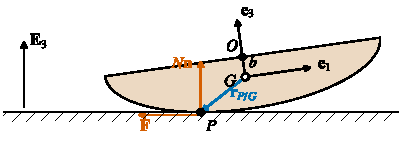
\includegraphics[width=\columnwidth]{figs/fig1_schematic.pdf}
\caption{Section of the rattleback in the $\ve e_1$--$\ve e_3$ plane, not to scale and
with the tilt exaggerated. $O$ is the center of the ellipsoid, $G$ the center of mass,
and $P$ the contact point. In the slipping formulation the contact force consists of a
normal reaction $N\ve n$ and a tangential friction force $\ve F$.}
\label{fig:schematic}
\end{figure}

\subsection{Elimination of the contact force}

Rolling without slipping, $\ve v_P=\ve 0$, fixes the velocity and acceleration of $G$ in
terms of the rotation,
\begin{align}
\ve v_G&=-\bm\omega\times\rpg,\label{eq:rollingvG}\\
\ve a_G&=-\dot{\bm\omega}\times\rpg-\bm\omega\times(\bm\omega\times\rpg)
          -\bm\omega\times\rdot.\label{eq:rollingaG}
\end{align}
The balance of linear momentum, $\ve f_P-mg\,\ve n=m\ve a_G$, is substituted into the
balance of angular momentum about $G$,
$\rpg\times\ve f_P=\ve I\dot{\bm\omega}+\bm\omega\times\ve I\bm\omega$, where $\ve I$ is
the inertia tensor about $G$. The contact force $\ve f_P$ then drops out, and
\cite{Kane1982,Mukherjee}
\begin{equation}
\bigl(\ve I-m\ve X^2\bigr)\dot{\bm\omega}=mg\,\ve X\ve n-m\ve X\ve W^2\rpg
-m\ve X\ve W\rdot-\ve W\ve I\bm\omega,
\label{eq:rolling}
\end{equation}
where $\ve X$ and $\ve W$ are the skew-symmetric matrices of $\rpg$ and $\bm\omega$.
Together with the Euler-angle kinematics, Eq.~\eqref{eq:rolling} is a system of six
first-order equations.

Two features of Eq.~\eqref{eq:rolling} matter for what follows. First, the added inertia
$-m\ve X^2$ and the terms $\ve X\ve W^2\rpg$ and $\ve X\ve W\rdot$ arise from eliminating
$\ve a_G$ through the constraint; they are not separate physical effects. Second, the
contact force is never computed, so the model gives no direct access to the normal
reaction or to the tangential force required to sustain rolling.

%=======================================================================
\section{Slipping-contact formulation}\label{sec:slip}
%=======================================================================

\subsection{Releasing the rolling constraint}

A Coulomb friction force has the form $\ve F=-\mu N\,\ve v_P/|\ve v_P|$. Under rolling,
$\ve v_P\equiv\ve 0$: the expression is undefined and, more fundamentally, there is no
relative motion for friction to oppose, so a rolling body dissipates nothing at the
contact. Moffatt and Shimomura make the same point for the spheroid \cite{Moffatt2002}.
In their analysis the slip velocity of the contact point reduces at leading order to a
single horizontal component, and it is the frictional force opposing this slip that
drives the secular rise; setting the slip to zero removes the mechanism.

Friction can therefore be introduced only after the constraint is released. Two things
follow. The velocity of the center of mass, $\ve v\equiv\ve v_G$, is no longer
determined by $\bm\omega$ and becomes an independent variable, which adds three states
to give the nine-state system
\begin{equation}
\ve y=[\omega_1\ \omega_2\ \omega_3\ \phi\ \theta\ \psi\ v_1\ v_2\ v_3]^{\top},
\label{eq:state}
\end{equation}
with $\ve v$ stored in body components. And the contact force can no longer be
eliminated, so it has to be constructed explicitly. The balance of angular momentum
returns to its plain form,
\begin{equation}
\ve I\dot{\bm\omega}+\bm\omega\times\ve I\bm\omega=\rpg\times\ve f_P+\ve T,
\label{eq:amb}
\end{equation}
in which the terms specific to rolling in Eq.~\eqref{eq:rolling} no longer appear and
$\ve T$ is an optional torque about the contact normal, used below for drilling friction.

\subsection{Decomposition of the contact force}

We write $\ve f_P=N\ve n+\ve F$ with $\ve F\cdot\ve n=0$, where $N$ is the normal
reaction and $\ve F$ the tangential friction force. The slip velocity of the material
point at $P$ and its tangential part are
\begin{align}
\ve v_P&=\ve v+\bm\omega\times\rpg,\label{eq:slip}\\
\ve v_P^{\,t}&=\ve v_P-(\ve v_P\cdot\ve n)\,\ve n .\label{eq:sliptan}
\end{align}
The normal component of $\ve v_P$ vanishes for an exact solution; the projection in
Eq.~\eqref{eq:sliptan} removes any residual arising from numerical drift.

\subsection{Normal reaction from the contact condition}\label{sec:normal}

Moffatt and Shimomura take the normal reaction to be of order $Mg$ \cite{Moffatt2002}.
This is a leading-order statement within their gyroscopic-balance approximation, in which
fast oscillations are averaged out. A rattleback, however, reverses through exactly such
oscillations, and Sec.~\ref{sec:normalresults} shows its normal reaction varying by a
factor of almost $30$ in a single run.

The normal reaction is a constraint force: it takes whatever value keeps $P$ on the
plane. The height of $G$ above the plane follows from the geometry alone,
\begin{equation}
z_G=h(\ve n)=\Bigl(\sum_i a_i^2n_i^2\Bigr)^{1/2}-b\,n_3=-\rpg\cdot\ve n .
\label{eq:height}
\end{equation}
Differentiating once and using $\rdot\cdot\ve n=0$, which holds because $\rdot$ is
tangent to the surface at $P$, gives $\dot z_G=-\rpg\cdot\dot{\ve n}$. A second
differentiation with $\ddot{\ve n}=-\dot{\bm\omega}\times\ve n-\bm\omega\times\dot{\ve
n}$ yields an expression linear in $\dot{\bm\omega}$,
\begin{equation}
\ddot z_G=c+\ve d\cdot\dot{\bm\omega},
\label{eq:zdd}
\end{equation}
\begin{equation}
c=-\rdot\cdot\dot{\ve n}+\rpg\cdot(\bm\omega\times\dot{\ve n}),\qquad
\ve d=\ve n\times\rpg .
\label{eq:cd}
\end{equation}
Both coefficients involve only quantities that the rolling formulation already
computes.

Because $\ve F$ is tangential, the vertical balance of linear momentum reads
\begin{equation}
N-mg=m\ddot z_G .
\label{eq:vertical}
\end{equation}
For Coulomb friction both $\ve F$ and the drilling torque are proportional to $N$, so
substituting $\ve f_P$ into Eq.~\eqref{eq:amb} makes $\dot{\bm\omega}$ affine in $N$,
\begin{equation}
\dot{\bm\omega}=\ve A_0+N(\ve B+\ve A_1),
\label{eq:affine}
\end{equation}
with
\begin{equation}
\begin{aligned}
\ve A_0&=-\ve I^{-1}(\bm\omega\times\ve I\bm\omega),\qquad
\ve B=\ve I^{-1}(\rpg\times\ve n),\\
\ve A_1&=\ve I^{-1}\bigl[\rpg\times\hat{\ve F}+\hat{\ve T}\bigr],
\end{aligned}
\label{eq:AB}
\end{equation}
where $\hat{\ve F}=\ve F/N$ and $\hat{\ve T}=\ve T/N$. Combining
Eqs.~\eqref{eq:zdd}--\eqref{eq:affine} gives a single scalar equation for $N$, whose
solution is
\begin{equation}
N=\frac{m\,(g+c+\ve d\cdot\ve A_0)}{1-m\,\ve d\cdot\ve B-m\,\ve d\cdot\ve A_1}.
\label{eq:N}
\end{equation}
Its evaluation costs one division per right-hand-side call and involves neither
iteration nor approximation. For a tangential law that does not scale with $N$, such as
the viscous law below, the torque $\rpg\times\ve F$ is moved into $\ve A_0$ and
$\ve A_1=\ve 0$.

\paragraph*{Well-posedness.}
Because $\ve B=-\ve I^{-1}\ve d$ and $\ve I$ is positive definite,
$-m\,\ve d\cdot\ve B=m\,\ve d^{\top}\ve I^{-1}\ve d\ge0$. In the frictionless case the
denominator of Eq.~\eqref{eq:N} is therefore at least $1$ and the solution always exists.
Friction adds the term $-m\,\ve d\cdot\ve A_1$, which could in principle make the
denominator vanish at large $\mu$. That situation is the rigid-body inconsistency of
Coulomb friction associated with Painlev\'e \cite{Stewart2000}, not a numerical failure.
The denominator was monitored in every computation and remained positive.

\subsection{Translational equation}

With $\ve v$ in body components, the balance of linear momentum becomes
\begin{equation}
\mathring{\ve v}=\frac{\ve f_P}{m}-g\,\ve n-\bm\omega\times\ve v ,
\label{eq:trans}
\end{equation}
where the last term accounts for the rotation of the body frame. The Euler-angle
kinematics are unchanged. Equations~\eqref{eq:amb}, \eqref{eq:N}, and \eqref{eq:trans},
with the kinematics, close the nine-state system once $\ve F$ and $\ve T$ are specified.

\subsection{Tangential contact laws}\label{sec:laws}

\paragraph*{Regularized Coulomb friction.}
The first law of Ref.~\cite{Moffatt2002} is a Coulomb law of magnitude $\mu Mg$ directed
against the slip. We implement it as
\begin{equation}
\ve F=-\mu N\,\frac{\ve v_P^{\,t}}{\bigl(|\ve v_P^{\,t}|^2+\varepsilon^2\bigr)^{1/2}},
\label{eq:coulomb}
\end{equation}
where the velocity scale $\varepsilon$ smooths the sign function so that the equations
remain integrable through zero slip. The instantaneous $N$ of Eq.~\eqref{eq:N} replaces
$Mg$. In the gyroscopic-balance analysis this law yields their Eq.~(15),
$\tan\theta=-(a/b)\tan\mu q(t-t_0)$, a transition completed in the finite interval
$\Delta t=\pi/2|\mu q|$ \cite{Moffatt2002}.

\paragraph*{Viscous friction.}
The second law of Ref.~\cite{Moffatt2002} is linear in the slip velocity. We write it as
\begin{equation}
\ve F=-c_v\,\ve v_P^{\,t}
\label{eq:viscous}
\end{equation}
with a constant coefficient $c_v$. It requires no regularization and is independent of
$N$, so it enters $\ve A_0$ and Eq.~\eqref{eq:N} applies with $\ve A_1=\ve 0$. In the
gyroscopic-balance analysis it yields their Eq.~(16), $\tan\theta=e^{-\mu q(t-t_0)}$, an
asymptotic approach on the secular time scale $|\mu q|^{-1}$ \cite{Moffatt2002}. The two
laws therefore differ in how they behave as the slip vanishes: the Coulomb force keeps
magnitude $\mu N$ down to slip speeds of order $\varepsilon$, whereas the viscous force
decreases in proportion to the slip.

\paragraph*{Drilling friction.}
A rigid point contact transmits no torque about the normal. A real contact occupies a
small patch, and when the patch rotates relative to the table the friction distributed
over it produces a torque about $\ve n$ that opposes the spin component
$\omega_n=\bm\omega\cdot\ve n$. This torque is absent from Ref.~\cite{Moffatt2002}.
Garcia and Hubbard included lumped spinning and slipping torques in their rattleback
equations on the grounds that the contact is an area rather than a point
\cite{Garcia1988}. The coupling between sliding and pivoting friction was analyzed by
Contensou \cite{Contensou1963}, developed by Zhuravlev into the Coulomb--Contensou model
\cite{Zhuravlev1998}, and applied to the celt with an elliptic contact patch by Kudra and
Awrejcewicz \cite{Kudra2015}. We use a single regularized term,
\begin{equation}
\ve T=-\mu N\rho\,
\frac{\rho\,\omega_n}{\bigl(\rho^2\omega_n^2+|\ve v_P^{\,t}|^2+\varepsilon^2\bigr)^{1/2}}\,\ve n,
\label{eq:drill}
\end{equation}
where $\rho$ is an effective lever arm. The denominator weakens the torque when sliding
dominates, which reproduces qualitatively the saturation of the Coulomb--Contensou
analysis. It is not the integral model or its Pad\'e approximants
\cite{Zhuravlev1998,Kudra2015}, and we use it as a sensitivity study.

The lever arm can be estimated from Hertzian contact \cite{Johnson1985}. For a fully
sliding circular patch of radius $a_H$ under a Hertzian pressure distribution,
integrating the Coulomb traction gives a torque $(3\pi/16)\mu Na_H$, so
$\rho=(3\pi/16)a_H$. At the lowest point of the ellipsoid the principal radii of
curvature are $a_1^2/a_3=2.0$\,m and $a_2^2/a_3=0.045$\,m, with geometric mean
$R_e=0.30$\,m. With $a_H=(3NR_e/4E^*)^{1/3}$ and $N=mg$, the patch radius is
$a_H\approx0.27$\,mm for steel on steel ($E^*\approx115$\,GPa) and $a_H\approx0.88$\,mm
for a polymer body ($E\approx3$\,GPa) on glass, giving $\rho\approx0.16$--$0.52$\,mm. We
take $\rho=0.5$\,mm as the representative value and examine $0\le\rho\le2$\,mm.

\subsection{Consistency with the rolling limit}

As $\mu\to\infty$ the slip velocity tends to zero and the slipping formulation must
reproduce Eq.~\eqref{eq:rolling}. This holds by construction, since
Eq.~\eqref{eq:rolling} follows from Eq.~\eqref{eq:amb} once the exact contact force of a
rolling body is substituted. The limit is the strongest test available, because it
exercises the geometry, the normal-reaction solution, and the friction law at once.

%=======================================================================
\section{Numerical method and verification}\label{sec:numerics}
%=======================================================================

\subsection{Parameters}

\begin{table}[!tbp]
\caption{Physical parameters, after Kane and Levinson \cite{Kane1982}. The product of
inertia carries the chirality; setting it to zero removes the reversal.}
\label{tab:params}
\begin{ruledtabular}
\begin{tabular}{lll}
Quantity & Symbol & Value \\
\hline
Mass & $m$ & $1$\,kg \\
Semi-axes & $a_1,a_2,a_3$ & $0.20,\ 0.03,\ 0.02$\,m \\
Offset of $O$ above $G$ & $b$ & $0.005$\,m \\
Moments of inertia & $I_{11},I_{22},I_{33}$ & $2.0,\ 16.0,\ 17.5\times10^{-4}$\,kg\,m$^2$ \\
Product of inertia & $I_{12}$ & $-0.5\times10^{-4}$\,kg\,m$^2$ \\
Initial spin & $\omega_0$ & $\pm5$\,rad\,s$^{-1}$ \\
Initial angles & $\phi,\theta,\psi$ & $10^{-6}$\,rad \\
\end{tabular}
\end{ruledtabular}
\end{table}

The physical parameters (Table~\ref{tab:params}) are those of Ref.~\cite{Kane1982}. The
sign of $I_{12}$ sets the preferred sense, which for these values is $\omega_3>0$; we
refer to $\omega_0=+5$\,rad\,s$^{-1}$ as the preferred sense and
$\omega_0=-5$\,rad\,s$^{-1}$ as the non-preferred sense.

\subsection{Implementation}

The slipping model integrates the state of Eq.~\eqref{eq:state}. Every run starts from
a rolling state, $\ve v(0)=-\bm\omega(0)\times\rpg(0)$, so that $\ve v_P(0)=\ve 0$ and the
slipping and rolling models share the same initial condition; the large-$\mu$ limit can
then be compared directly with the rolling solution. The geometric quantities $\ve n$,
$\dot{\ve n}$, $\rpg$, and $\rdot$ are computed by one routine shared by both models.
The rolling equations, Eq.~\eqref{eq:rolling}, are integrated alongside every slipping
run as a reference. Their contact force is recovered after integration from
$\ve f_P=m(\ve a_G+g\,\ve n)$ with $\ve a_G$ from Eq.~\eqref{eq:rollingaG}, which makes the
normal reaction and the friction demand of the rolling solution observable.

The regularized Coulomb law contributes Jacobian entries of order $\mu N/\varepsilon$,
about $5\times10^4$\,N\,s\,m$^{-1}$ at the values used here, and makes the slipping system
stiff. It was therefore solved with the variable-order backward-differentiation solver
\texttt{ode15s} of MATLAB \cite{Shampine1997}, with relative and absolute tolerances of
$10^{-8}$ and $10^{-10}$. For the Coulomb case the reversal time, final spin, and maximum
rocking angle were unchanged to four significant figures when the tolerances were varied
from $10^{-6}$ and $10^{-8}$ to $10^{-10}$ and $10^{-12}$. The non-stiff rolling model was solved with the explicit
Runge--Kutta pair \texttt{ode45} at tolerances of $10^{-10}$ and $10^{-12}$. Solutions
were written on a uniform grid of $20\,001$ points over $8$\,s. The solvers choose their
own internal steps, so the output grid does not affect accuracy; it gives about $250$
samples per period of the $11$\,Hz rocking, and the contact diagnostics below are
evaluated at every output point.

The numerical part of the MATLAB code was also run under GNU Octave 8.4 \cite{Eaton2023}, with the same results. An
independent Python implementation, using the LSODA integrator \cite{Petzold1983} of SciPy
\cite{Virtanen2020}, was written to cross-check the results and to render the
animations. The two implementations agree on reversal times to within $0.002$\,s and on
maximum rocking angles to within $0.01^\circ$. In the animations the orientation is
assembled as $\ve Q=\ve R_1(\phi)\ve R_2(\theta)\ve R_3(\psi)$, which reproduces
$\ve Q^{\top}\ve E_3=\ve n$ to machine precision, and the body is drawn at its computed
height $h(\ve n)$, so it rests on the plane by construction.

\subsection{Verification}\label{sec:validation}

Four checks were evaluated in every run.
(i) \emph{Contact residual.} The quantity $g_v=\ve v\cdot\ve n+\rpg\cdot\dot{\ve n}$,
the rate of change of the gap between $P$ and the plane, vanishes when Eq.~\eqref{eq:N}
is satisfied. Its maximum over all runs was below $2\times10^{-7}$\,m\,s$^{-1}$, of the order of the solver tolerance.
(ii) \emph{Energy.} The total energy
$E=\tfrac12\bm\omega\cdot\ve I\bm\omega+\tfrac12m|\ve v|^2+mgh$ was conserved in the
rolling model, with a drift below $10^{-10}$\,J over $8$\,s, and decreased monotonically
in every dissipative run.
(iii) \emph{Positive normal reaction.} $N>0$ throughout, so the body never left the plane
and the assumption of permanent contact is self-consistent. The denominator of
Eq.~\eqref{eq:N} also remained positive.
(iv) \emph{Rolling limit.} As $\mu$ increases, the Coulomb solution converges to the
rolling solution (Sec.~\ref{sec:mu}); at $\mu=1$ and $2$ the reversal time agrees with
the rolling value of $2.83$\,s to three significant figures.

\subsection{Convergence in the regularization}\label{sec:eps}

\begin{figure}[!tbp]
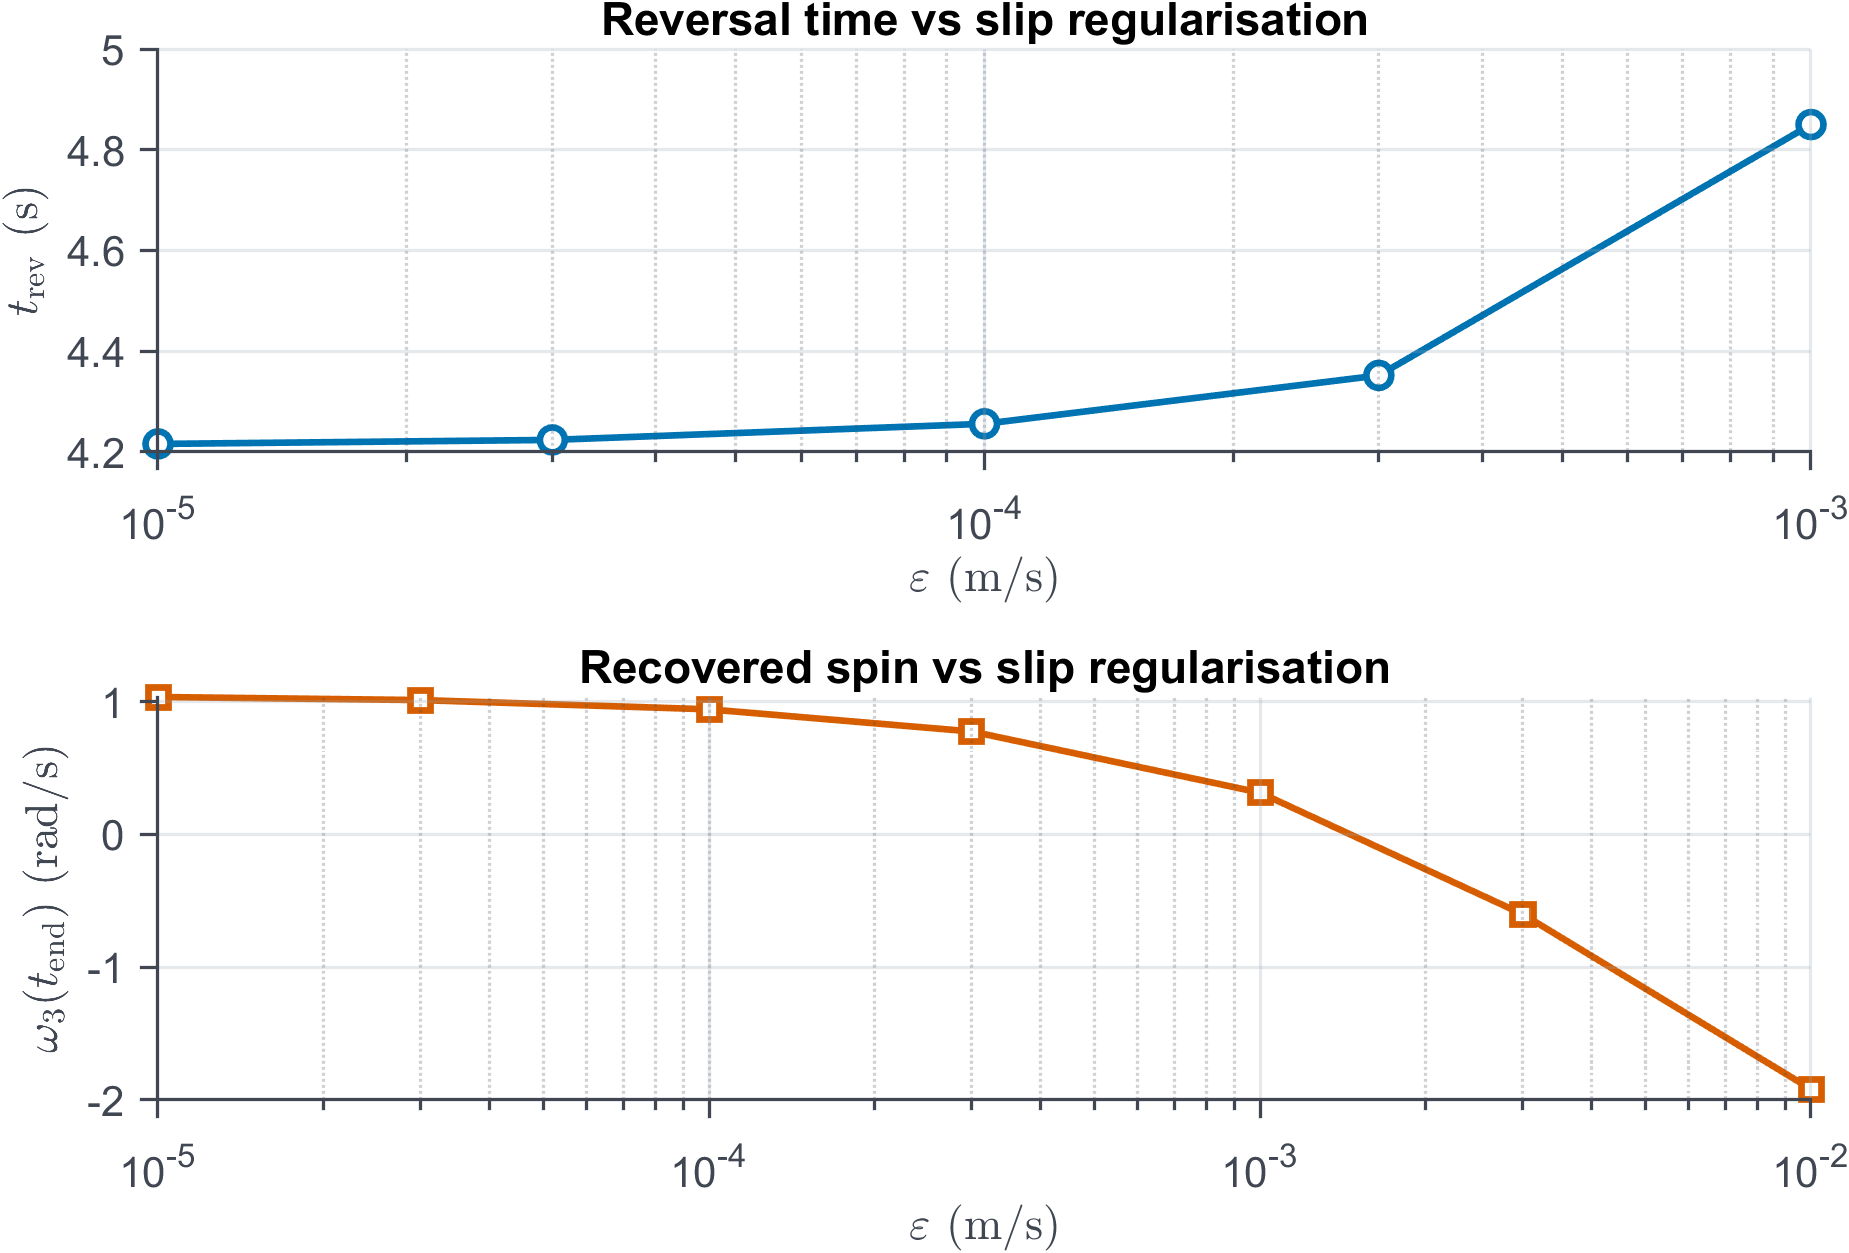
\includegraphics[width=\columnwidth]{figs/sweep_epsilon.png}
\caption{Convergence of the Coulomb model ($\mu=0.15$, non-preferred sense) in the
regularization velocity $\varepsilon$. Top: reversal time, the first zero crossing of
$\omega_3$; points are missing where no reversal occurs within $8$\,s. Bottom: spin at
$t=8$\,s.}
\label{fig:eps}
\end{figure}

\begin{table}[!tbp]
\caption{Dependence of the Coulomb solution ($\mu=0.15$, non-preferred sense) on the
regularization velocity $\varepsilon$. A dash denotes no reversal within $8$\,s.}
\label{tab:eps}
\begin{ruledtabular}
\begin{tabular}{lccccccc}
$\varepsilon$ (m\,s$^{-1}$) & $10^{-2}$ & $3\!\times\!10^{-3}$ & $10^{-3}$ &
$3\!\times\!10^{-4}$ & $10^{-4}$ & $3\!\times\!10^{-5}$ & $10^{-5}$ \\
\hline
$t_{\rm rev}$ (s) & -- & -- & 4.85 & 4.35 & 4.26 & 4.22 & 4.22 \\
$\omega_3(8\,{\rm s})$ & $-1.92$ & $-0.60$ & $0.32$ & $0.78$ & $0.94$ & $1.01$ & $1.04$ \\
\end{tabular}
\end{ruledtabular}
\end{table}

The regularization requires care (Fig.~\ref{fig:eps}, Table~\ref{tab:eps}). The
reversal time and the final spin depend strongly on $\varepsilon$ when it is comparable
to the slip speeds, which are of order $10^{-2}$\,m\,s$^{-1}$ during reversal. At
$\varepsilon=10^{-2}$ and $3\times10^{-3}$\,m\,s$^{-1}$ the smoothed law behaves like a
viscous law at small slip and the body does not reverse within $8$\,s. At
$\varepsilon=10^{-3}$\,m\,s$^{-1}$, a value that may appear small, the reversal occurs at
$4.85$\,s, about $15\%$ later than the converged value. Between $\varepsilon=3\times10^{-5}$
and $10^{-5}$\,m\,s$^{-1}$ the reversal time changes by $0.007$\,s and the final spin by
$0.02$\,rad\,s$^{-1}$. All Coulomb results below use
$\varepsilon=3\times10^{-5}$\,m\,s$^{-1}$.

%=======================================================================
\section{Results and discussion}\label{sec:results}
%=======================================================================

\begin{table*}[t]
\caption{Summary of results for $|\omega_0|=5$\,rad\,s$^{-1}$ over $8$\,s, with
$\varepsilon=3\times10^{-5}$\,m\,s$^{-1}$. $t_{\rm rev}$ is the first zero crossing of
$\omega_3$, $\theta_{\max}$ the maximum rocking angle, and $\Delta E/E_0$ the fractional
change of energy, with $E_0=0.169$\,J. Energy was conserved or decreased monotonically in
every run, and no contact law produced a reversal in the preferred sense.}
\label{tab:results}
\begin{ruledtabular}
\begin{tabular}{llccccc}
Contact law & Sense & $t_{\rm rev}$ (s) & $\omega_3(8\,{\rm s})$ (rad\,s$^{-1}$) &
$N/mg$ & $\theta_{\max}$ & $\Delta E/E_0$ \\
\hline
Rolling & preferred & -- & $+5.00$ & 1.00 & $<0.01^\circ$ & $0$ \\
Rolling & non-preferred & 2.83 & $+5.00$ & 0.20--5.86 & $6.48^\circ$ & $0$ \\
Coulomb, $\mu=0.15$ & preferred & -- & $+5.00$ & 1.00 & $<0.01^\circ$ & $0$ \\
Coulomb, $\mu=0.15$ & non-preferred & 4.22 & $+1.01$ & 0.76--1.30 & $0.84^\circ$ & $-12.4\%$ \\
Coulomb + drilling, $\rho=0.5$\,mm & preferred & -- & $+1.64$ & 1.00 & $<0.01^\circ$ & $-11.5\%$ \\
Coulomb + drilling, $\rho=0.5$\,mm & non-preferred & 3.98 & $+0.02$ & 0.76--1.30 & $0.84^\circ$ & $-12.9\%$ \\
Viscous, $c_v=500$\,kg\,s$^{-1}$ & preferred & -- & $+5.00$ & 1.00 & $<0.01^\circ$ & $0$ \\
Viscous, $c_v=500$\,kg\,s$^{-1}$ & non-preferred & 2.90 & $+1.40$ & 0.40--2.63 & $3.09^\circ$ & $-11.9\%$ \\
\end{tabular}
\end{ruledtabular}
\end{table*}

Table~\ref{tab:results} collects the results for the four contact models in both senses
of rotation. The subsections below discuss each model and then compare them.

\subsection{Rolling solution}

\begin{figure}[!tbp]
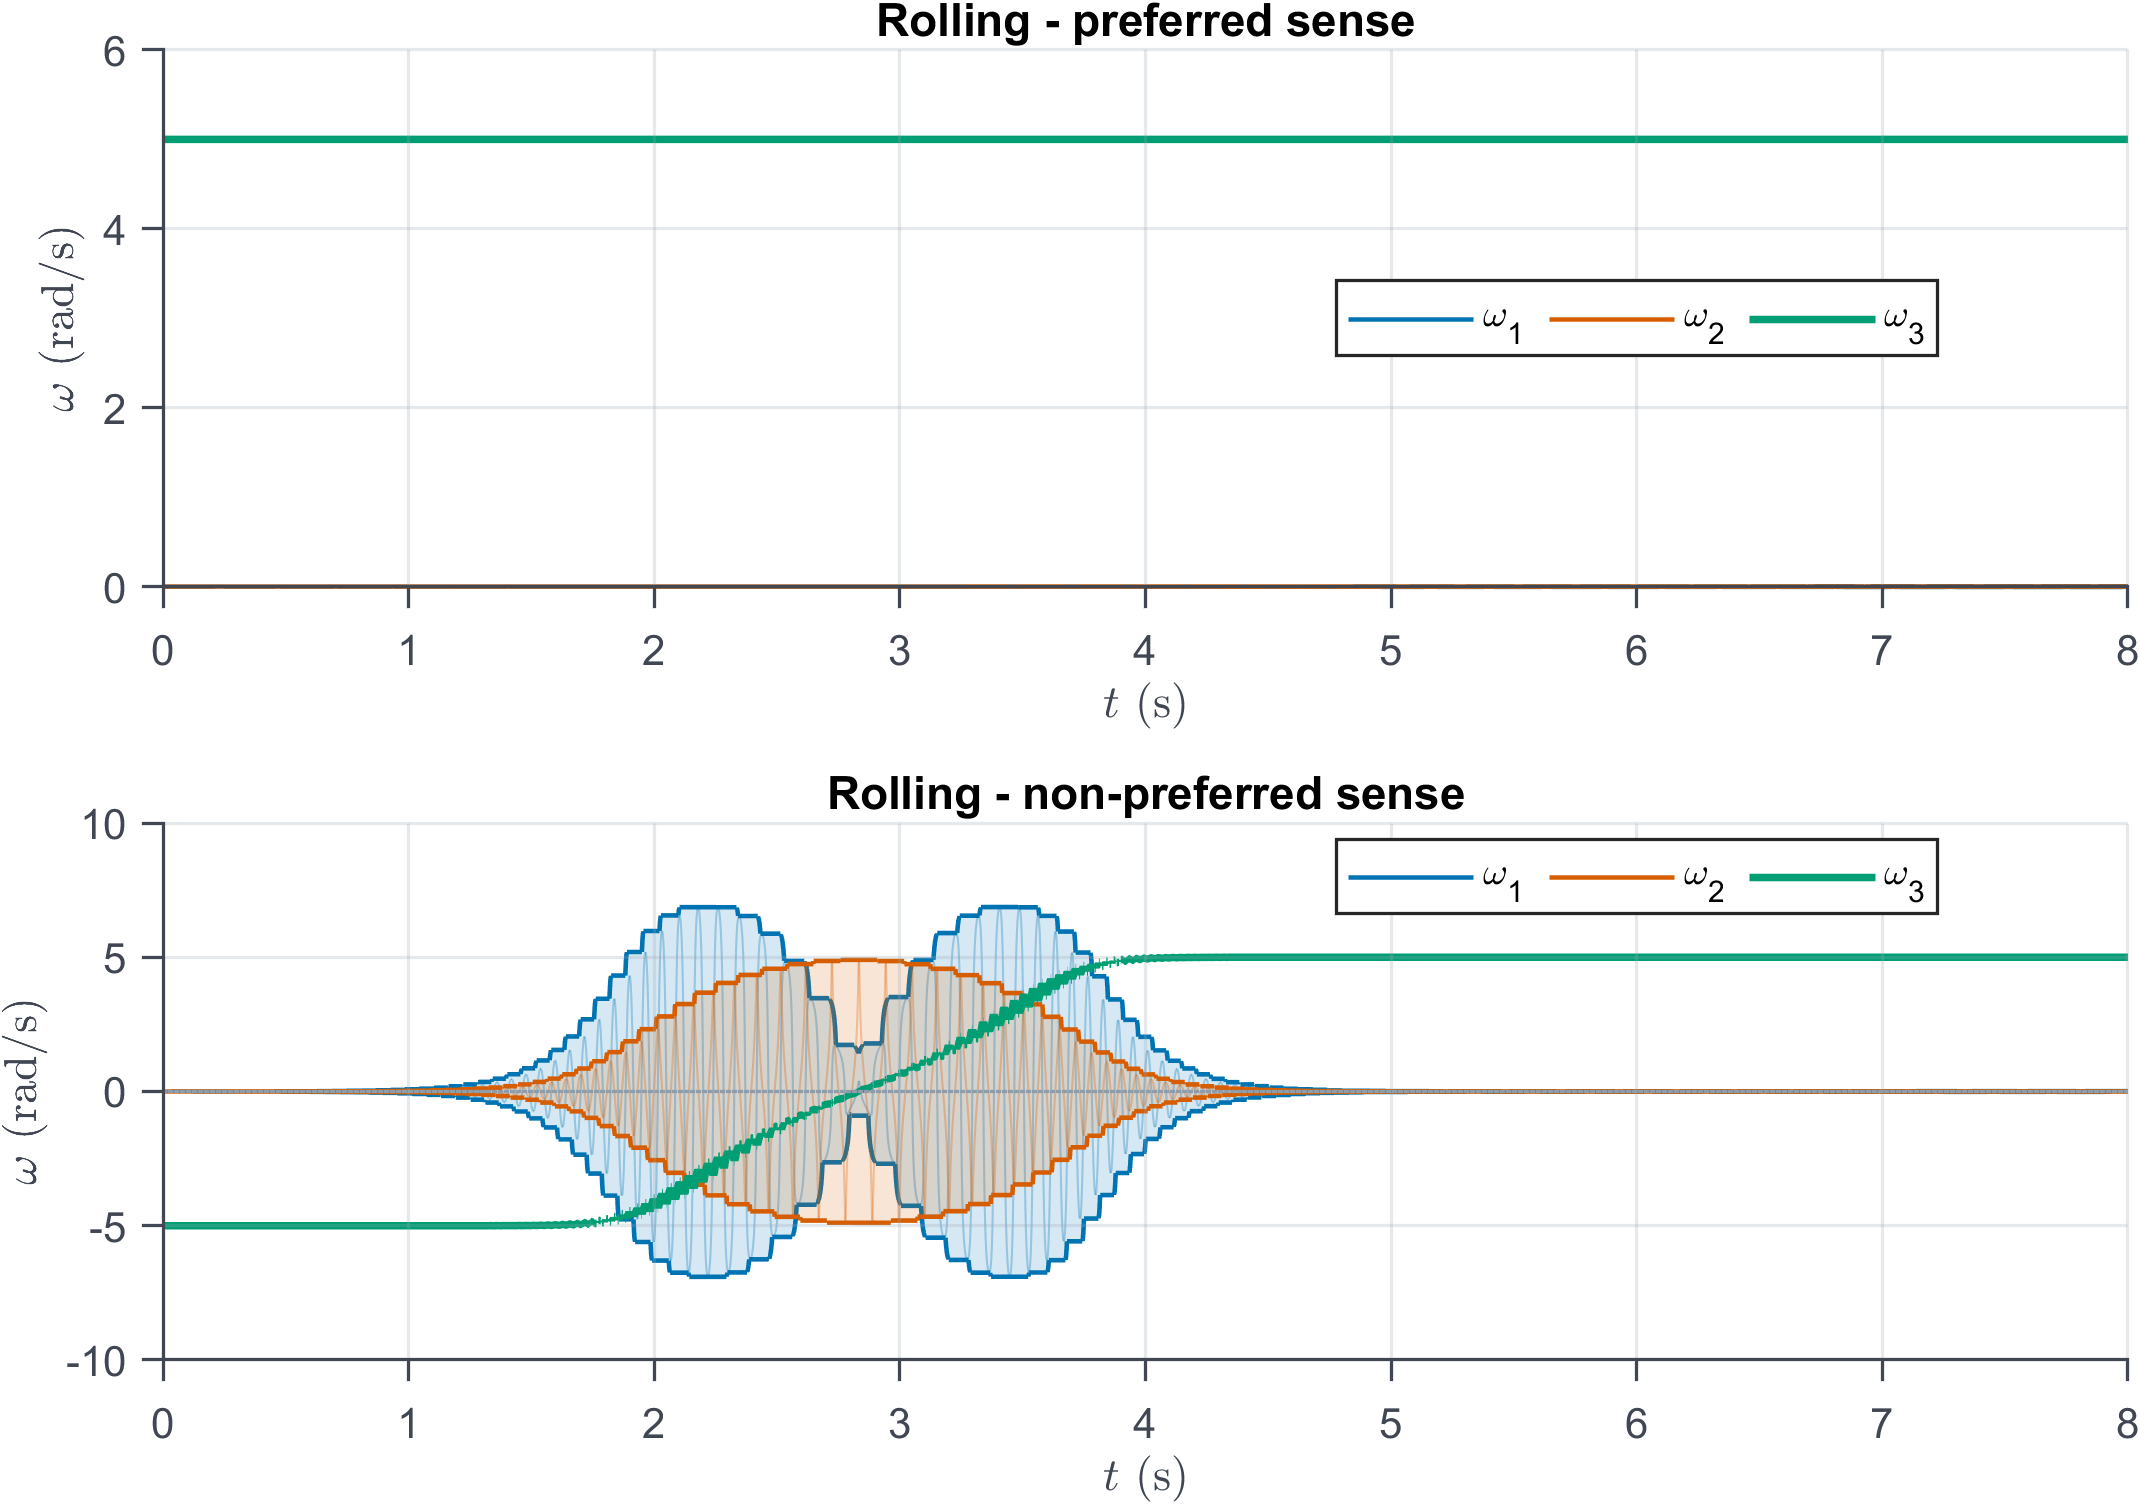
\includegraphics[width=\columnwidth]{figs/omega_rolling.png}\\[2pt]
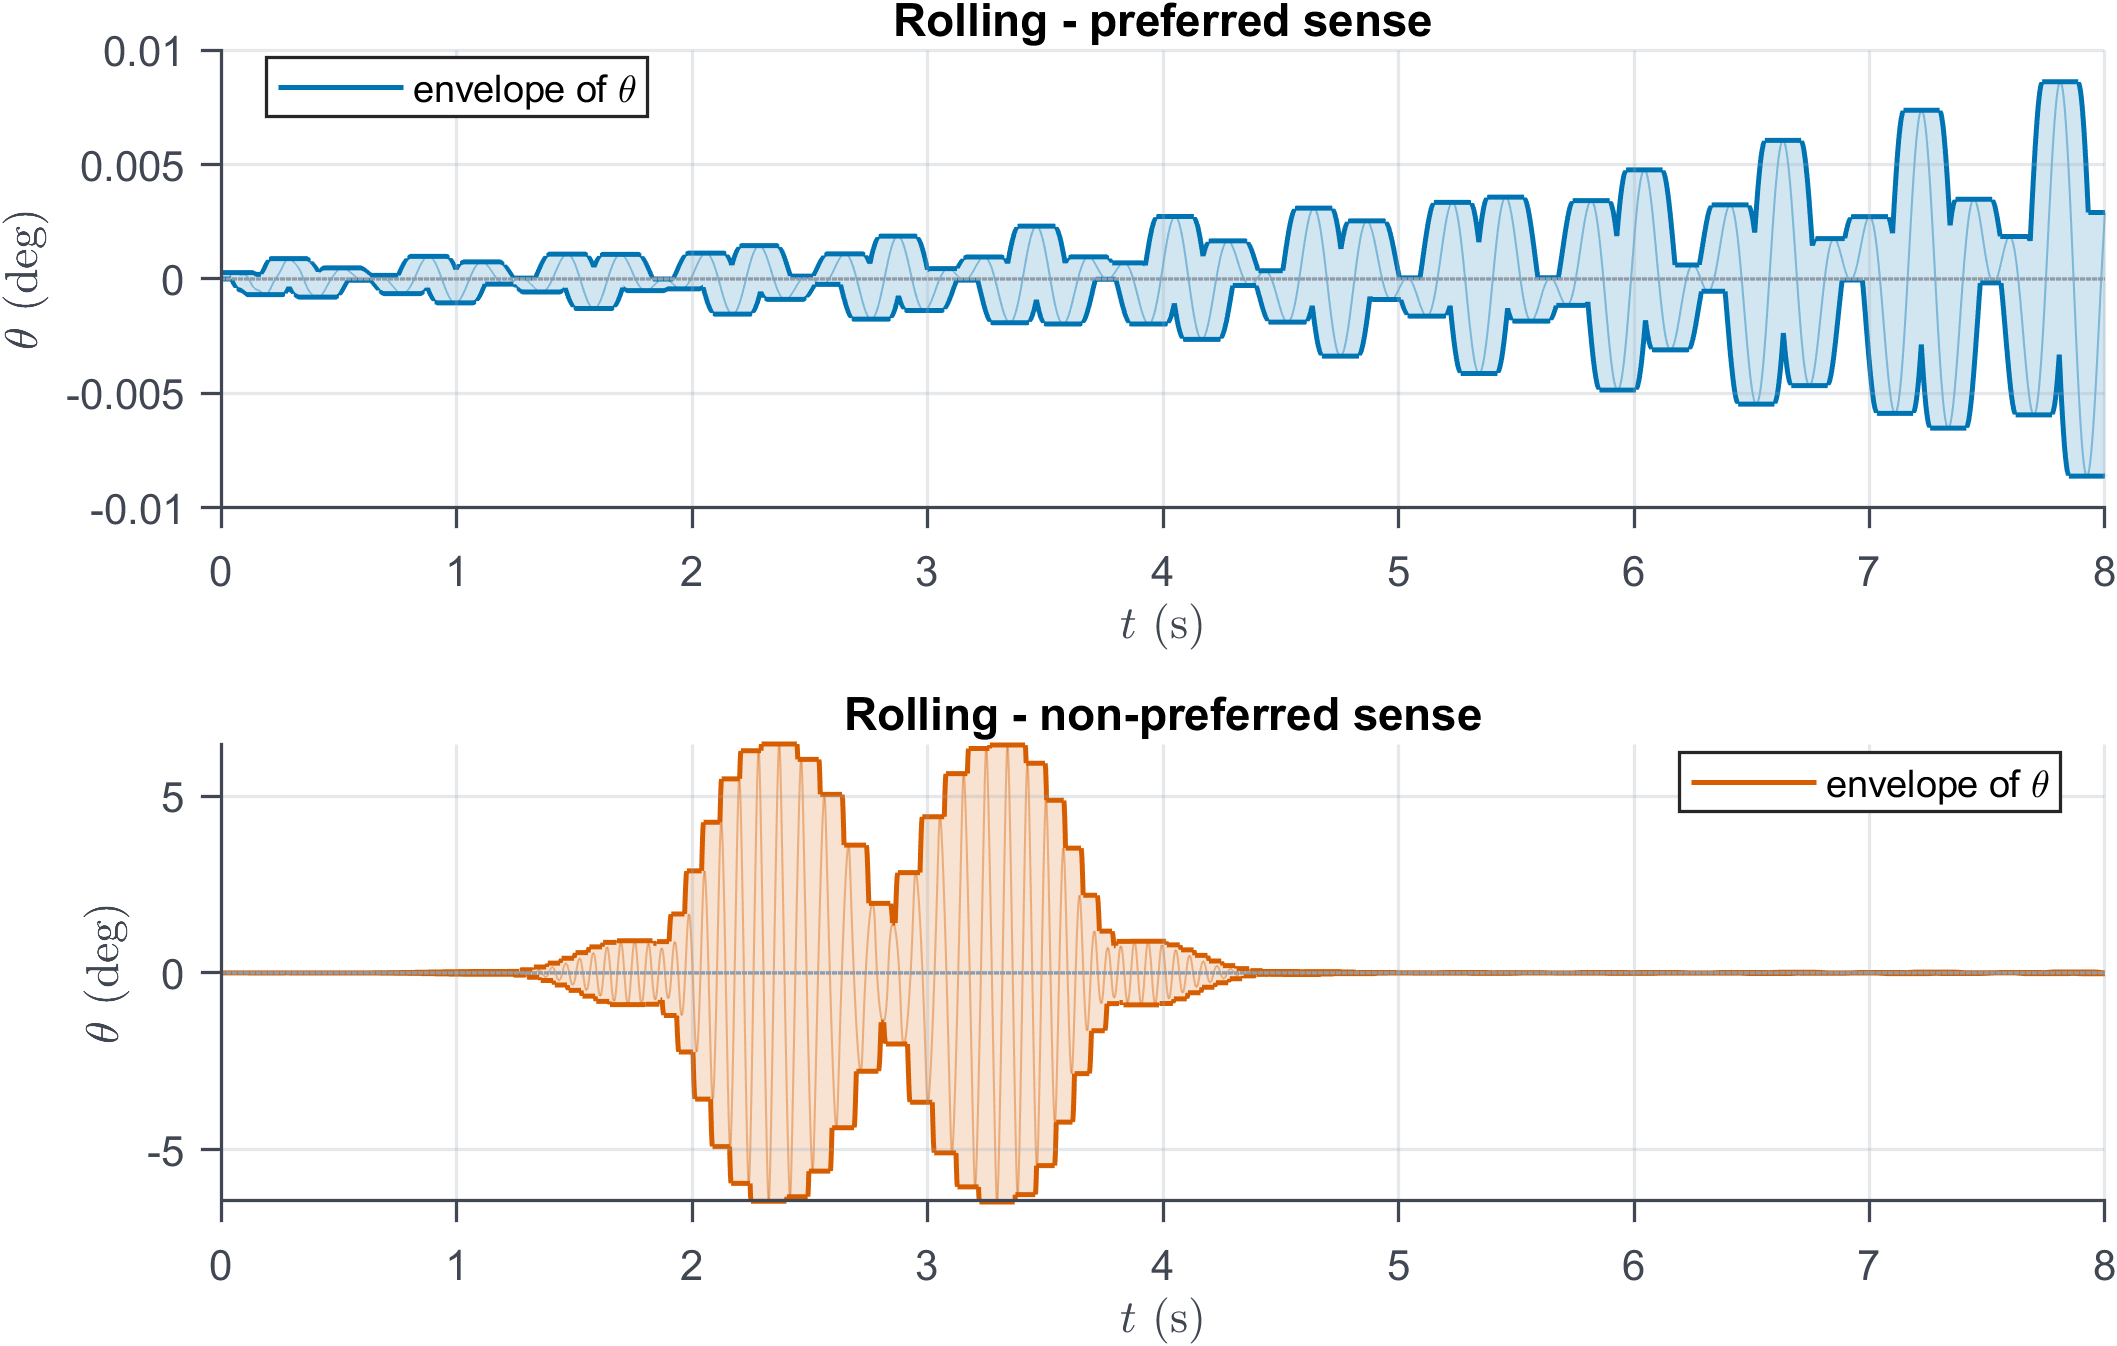
\includegraphics[width=\columnwidth]{figs/theta_rolling.png}
\caption{Rolling solution. Upper pair: angular velocity components in the preferred and
non-preferred senses. Lower pair: rocking angle $\theta$. In the preferred sense
$\omega_3$ stays at $+5$\,rad\,s$^{-1}$ with no oscillation. In the non-preferred sense
the spin reverses at $t=2.83$\,s, the energy passing through $\omega_1$ and $\omega_2$
oscillations of about $\pm7$ and $\pm5$\,rad\,s$^{-1}$ while $\theta$ reaches $6.5^\circ$.
Because the model is conservative, $\omega_3$ recovers its full magnitude.}
\label{fig:rolling}
\end{figure}

Figure~\ref{fig:rolling} shows the rolling solution. In the preferred sense the spin
remains at $5$\,rad\,s$^{-1}$ and the rocking angle stays below $0.01^\circ$. In the
non-preferred sense the rocking grows from $t\approx1.3$\,s, reaches
$\theta_{\max}=6.48^\circ$, and $\omega_3$ crosses zero at $t=2.83$\,s. The rocking then
decays and the spin settles at $+5$\,rad\,s$^{-1}$, its initial magnitude, as energy
conservation requires. This reproduces the rolling formulation of Ref.~\cite{Mukherjee}
and agrees with Ref.~\cite{Kane1982}.

\subsection{Coulomb friction}

\begin{figure}[!tbp]
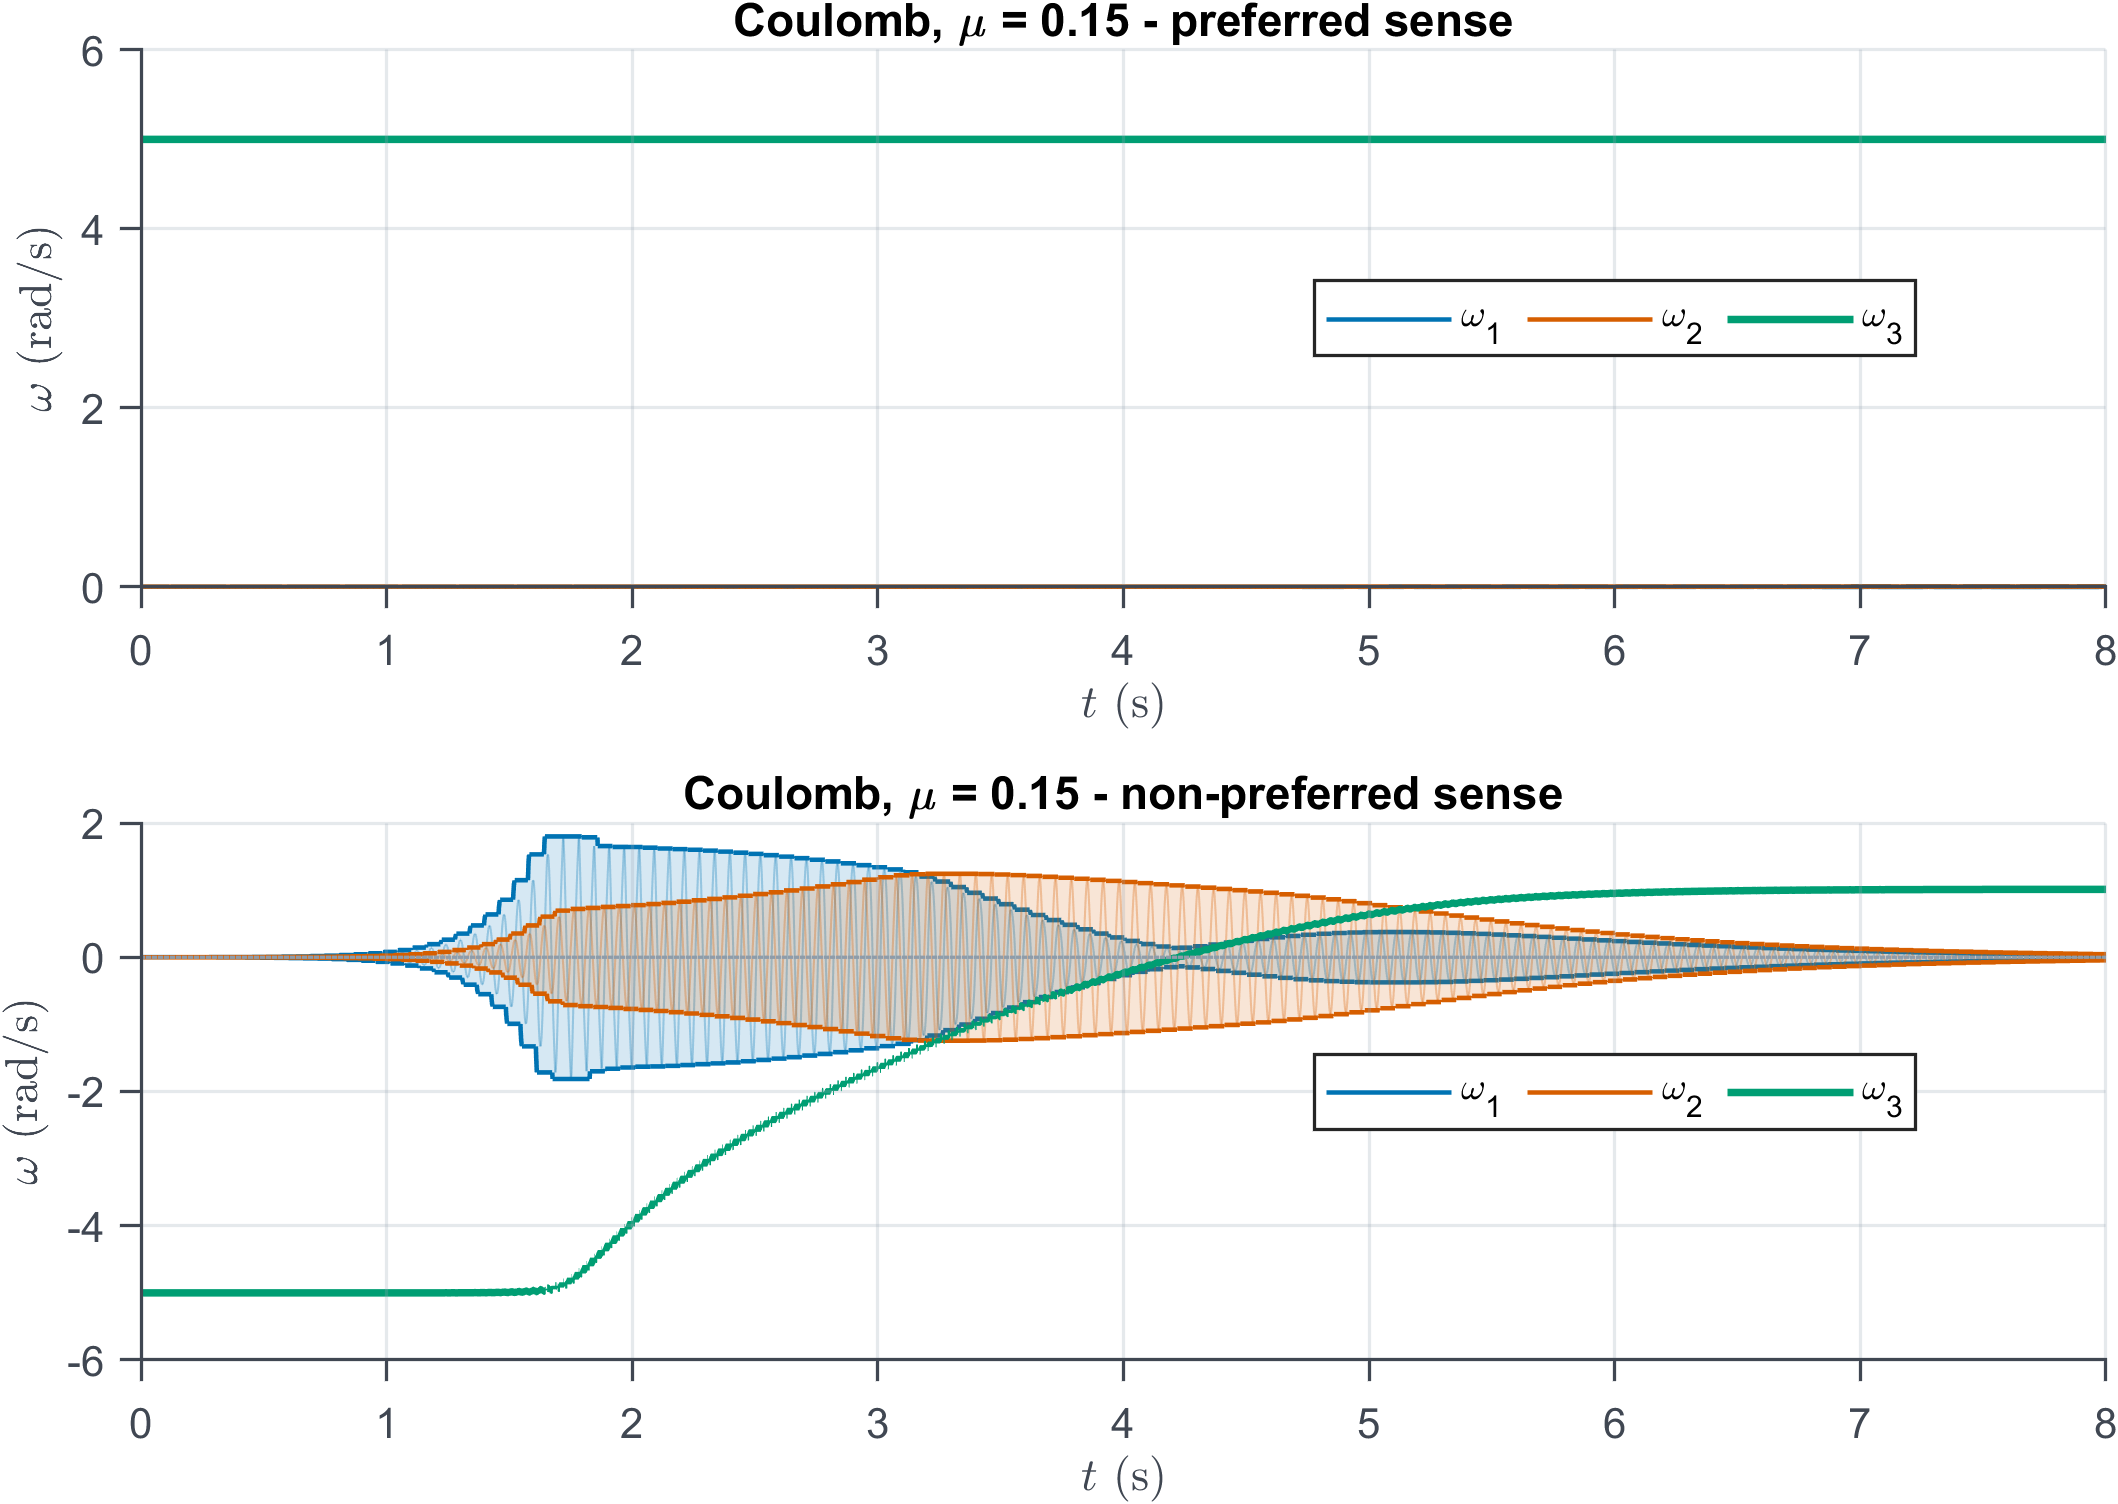
\includegraphics[width=\columnwidth]{figs/omega_coulomb.png}\\[2pt]
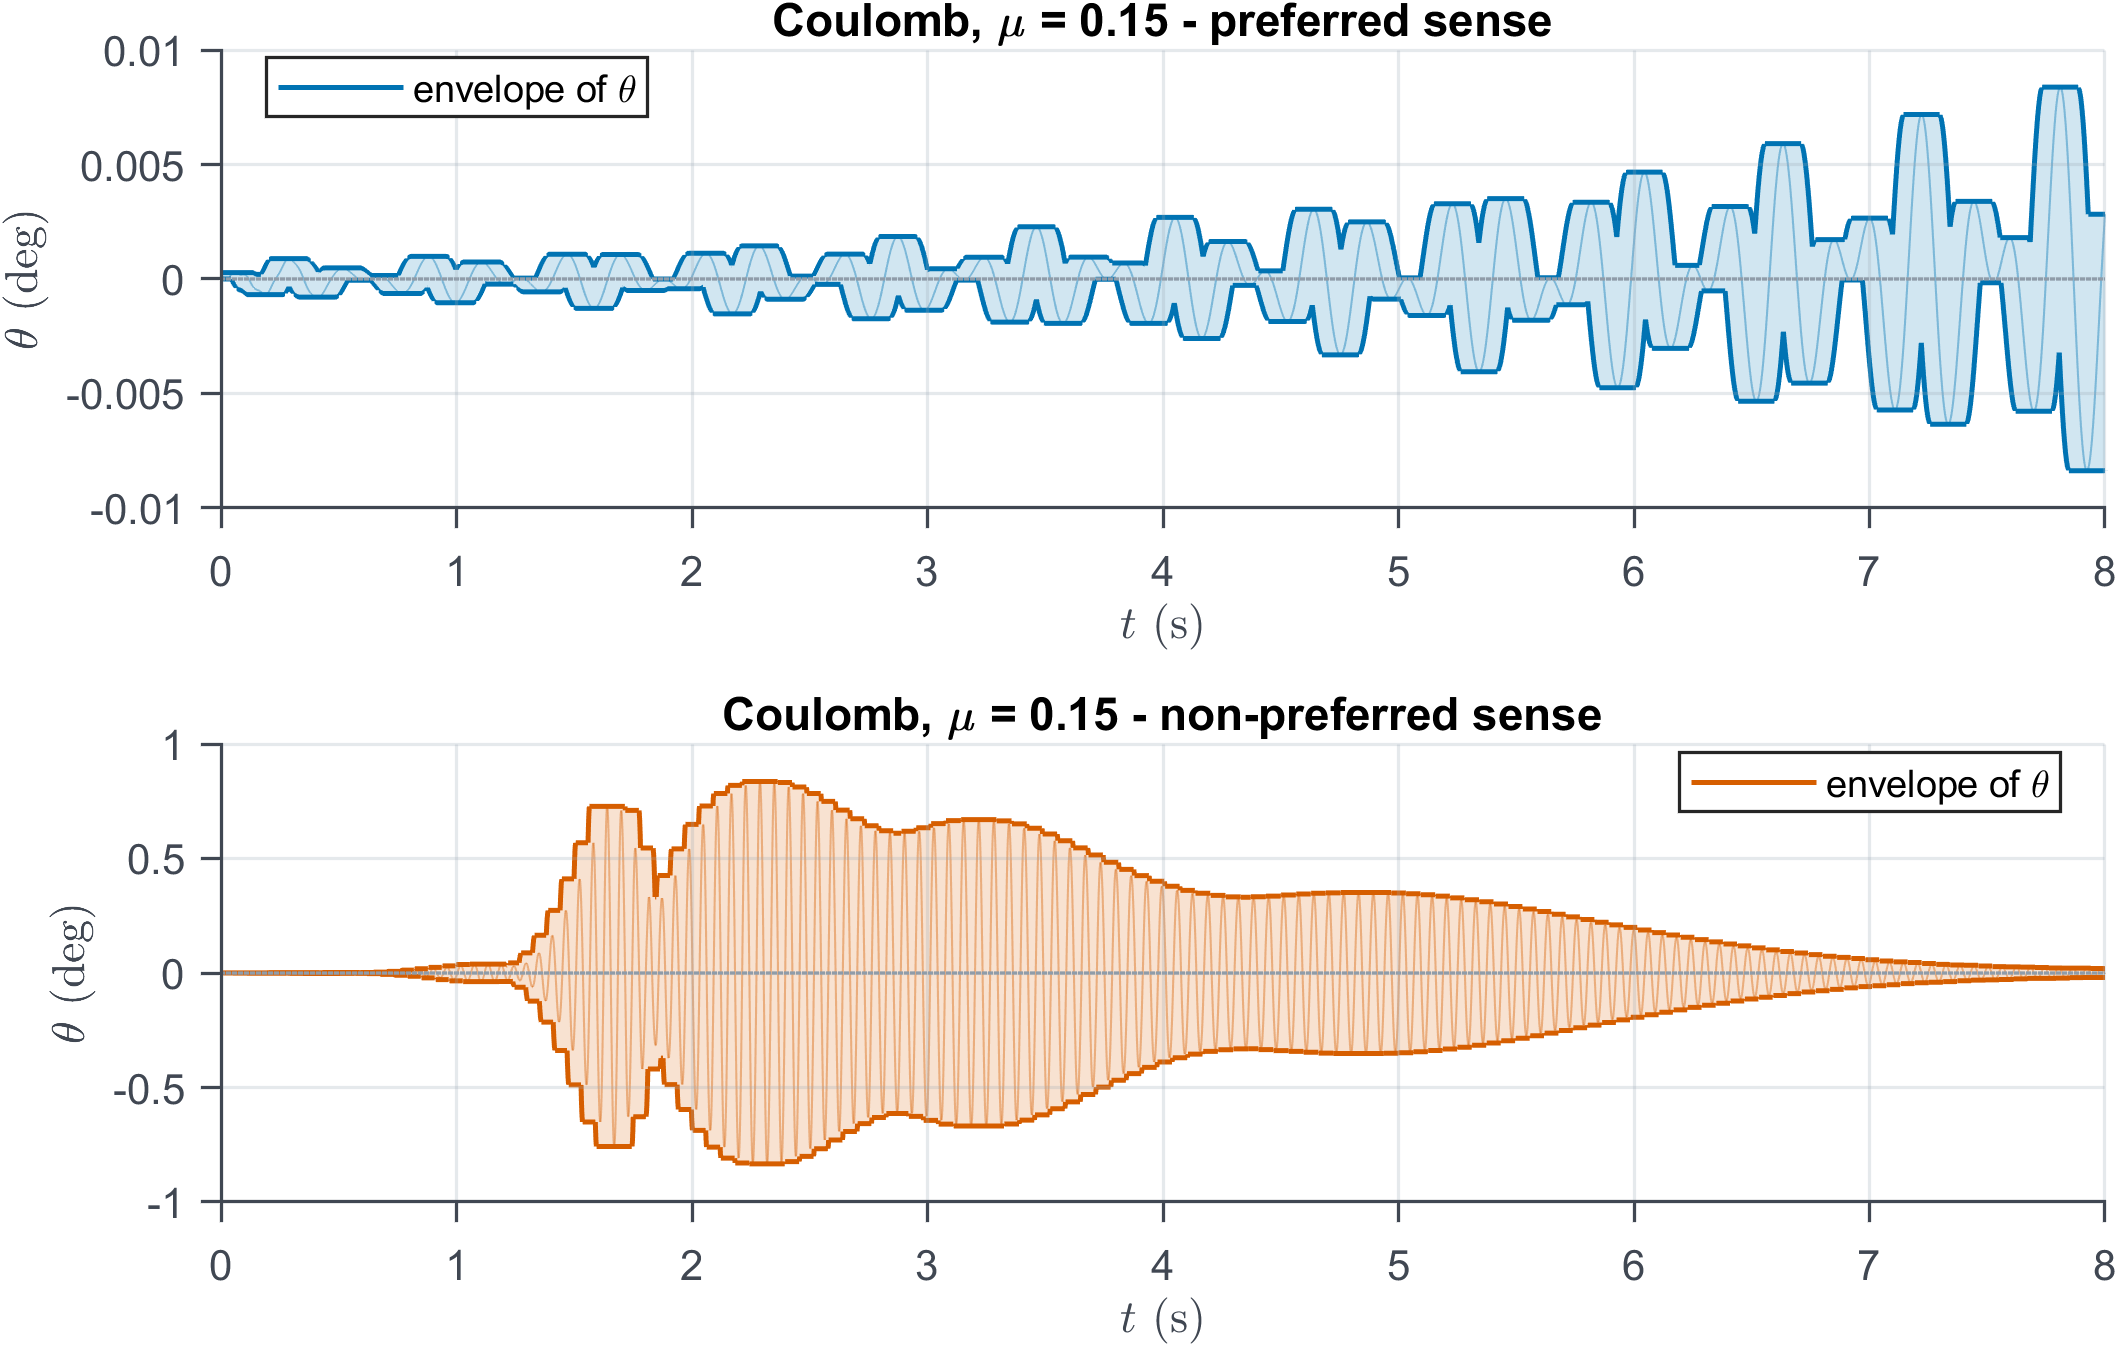
\includegraphics[width=\columnwidth]{figs/theta_coulomb.png}
\caption{Coulomb friction, $\mu=0.15$. Upper pair: angular velocity components. Lower
pair: rocking angle. The reversal occurs later than in rolling ($4.22$\,s against
$2.83$\,s), the rocking is limited to $0.84^\circ$, and the recovered spin is
$+1.01$\,rad\,s$^{-1}$ instead of $+5$\,rad\,s$^{-1}$.}
\label{fig:coulomb}
\end{figure}

\begin{figure}[!tbp]
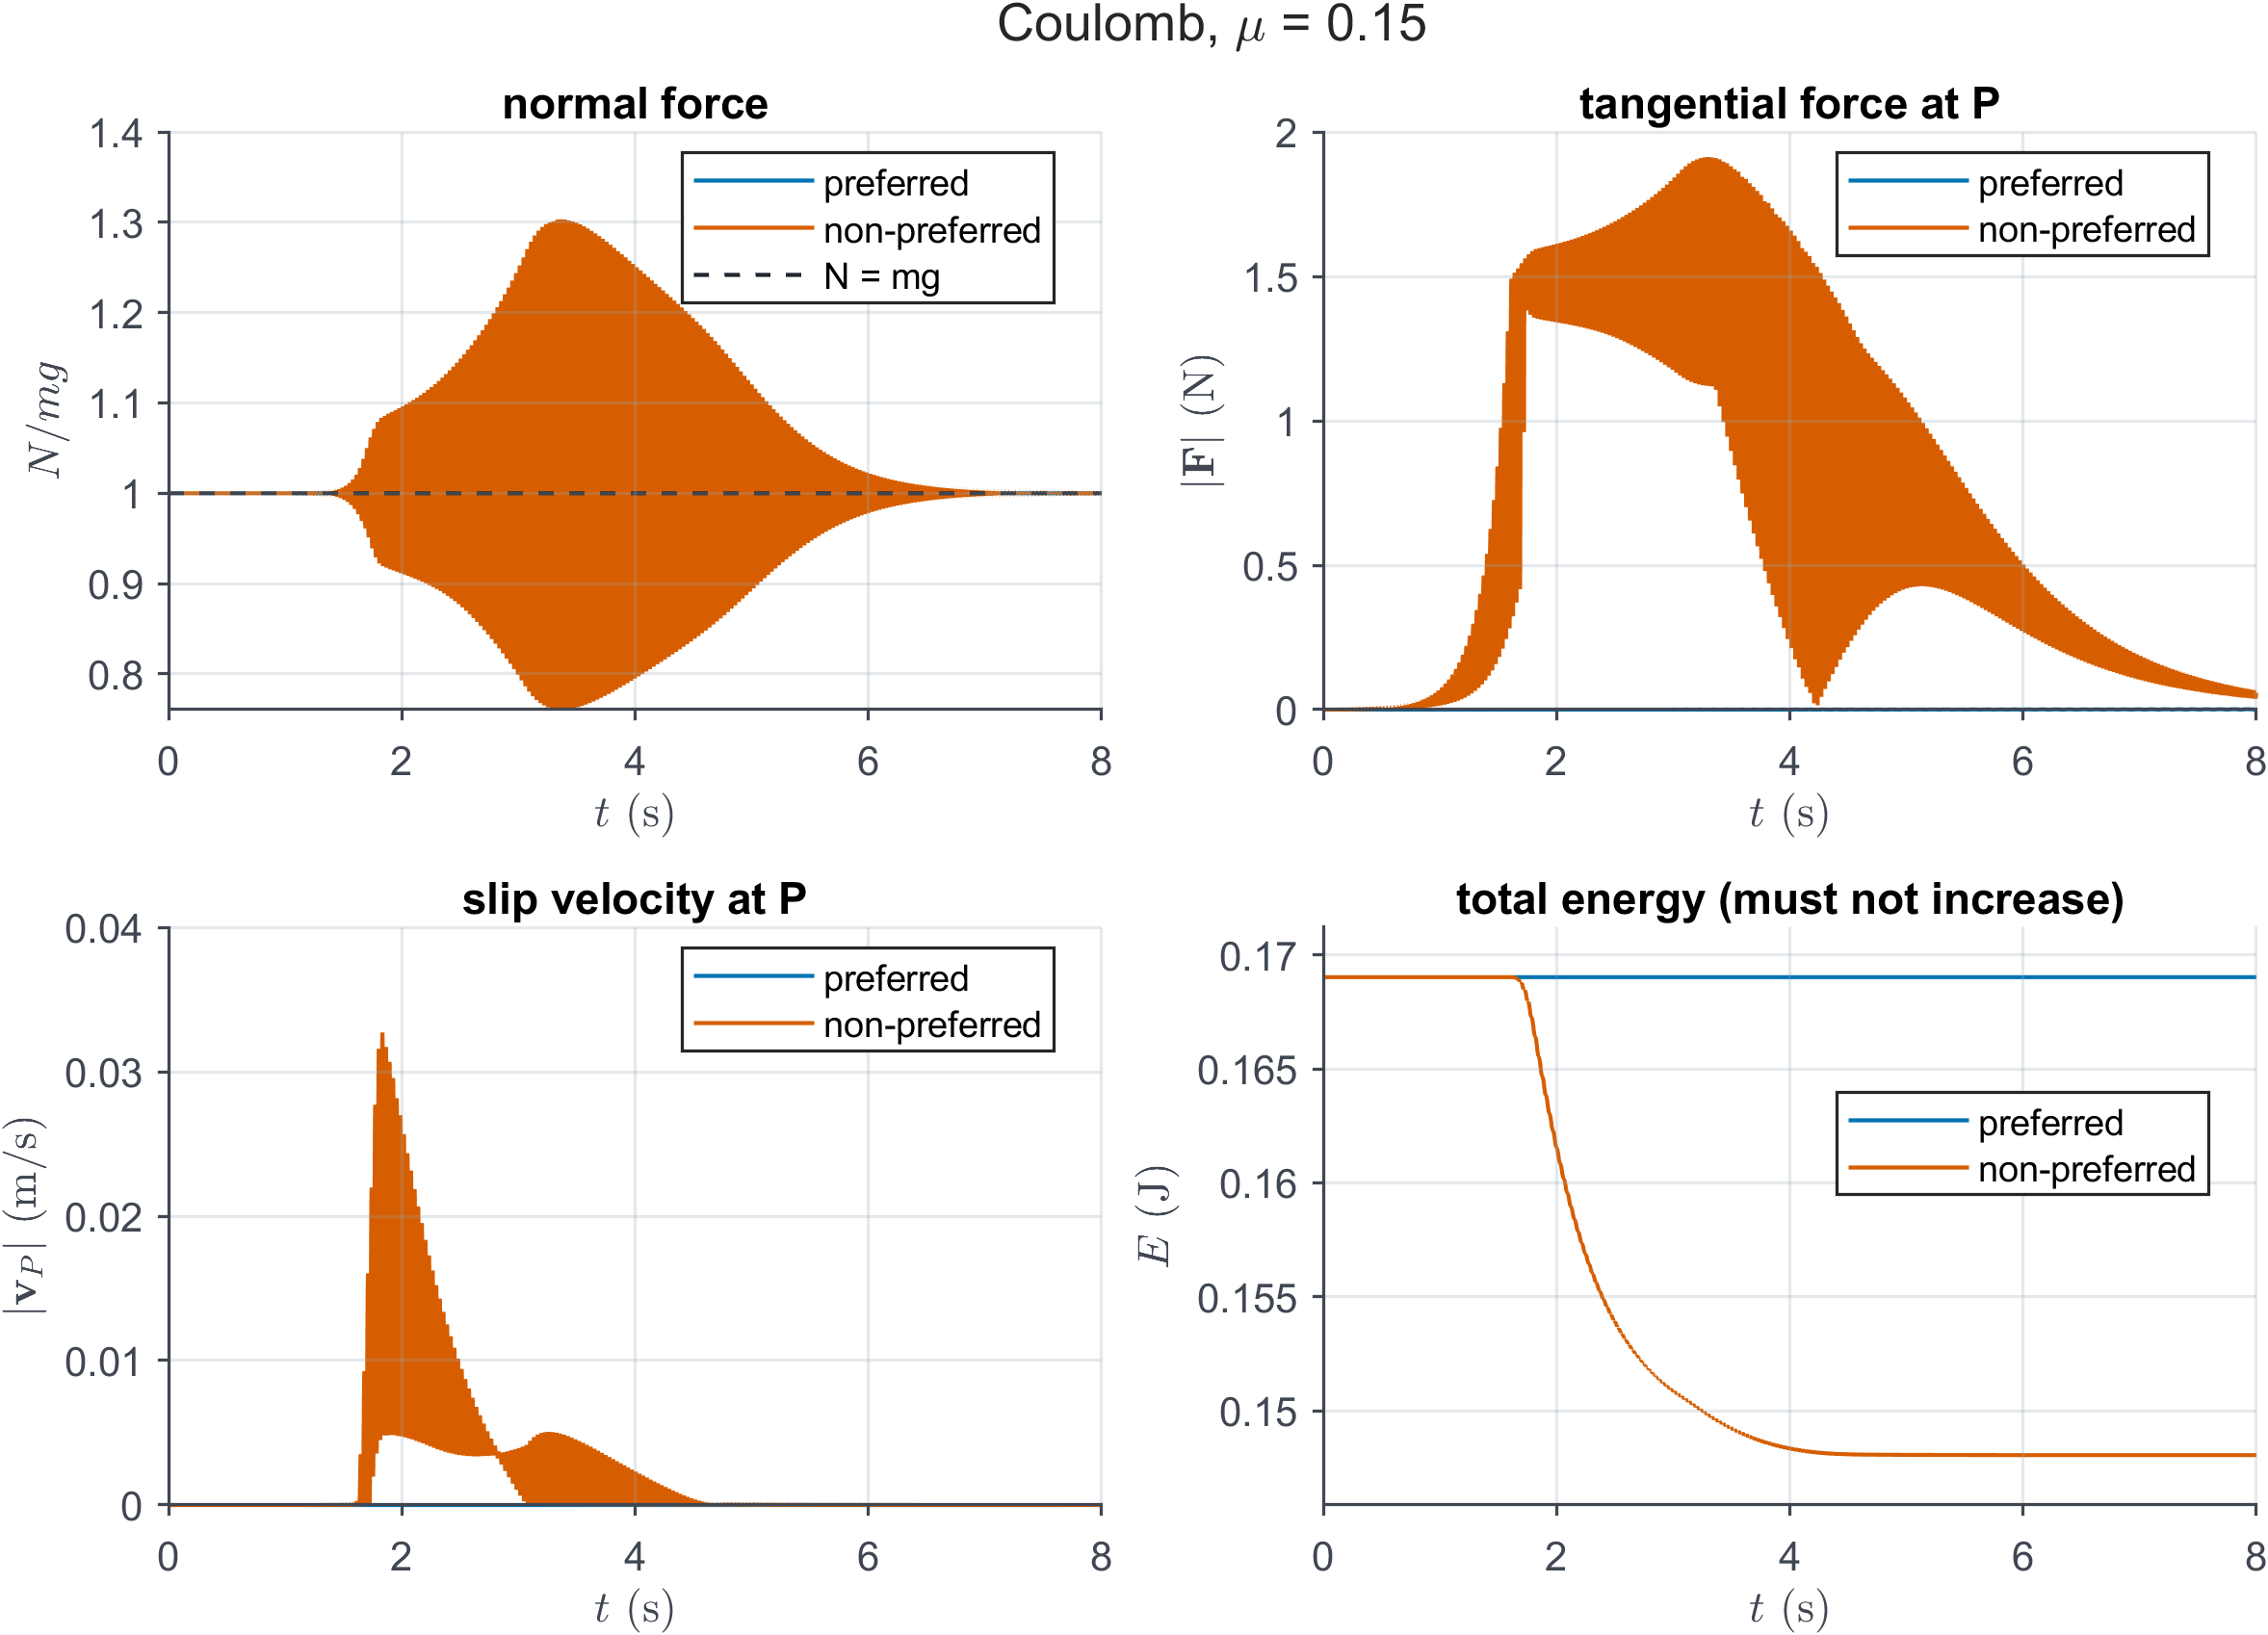
\includegraphics[width=\columnwidth]{figs/contact_coulomb.png}
\caption{Contact diagnostics for Coulomb friction, $\mu=0.15$: normal reaction relative to
$mg$, magnitude of the tangential force, slip speed of the contact point, and total
energy. The preferred sense is flat in every panel. In the non-preferred sense $N/mg$
ranges from $0.76$ to $1.30$, the slip reaches $32$\,mm\,s$^{-1}$, and the energy falls
monotonically by $12.4\%$.}
\label{fig:contactcoulomb}
\end{figure}

With Coulomb friction at $\mu=0.15$ (Figs.~\ref{fig:coulomb} and
\ref{fig:contactcoulomb}) the contact begins to slip as soon as the rocking grows, at
speeds of up to $32$\,mm\,s$^{-1}$. Friction limits the rocking to $0.84^\circ$, an
eighth of the rolling value. Two features deserve comment. First, the reversal is
delayed rather than accelerated, to $4.22$\,s from $2.83$\,s. Friction damps the very
oscillation that carries the energy exchange, so the instability takes longer to
complete. Second, the spin after reversal is a small fraction of the initial spin. About
$12\%$ of the initial energy is dissipated, almost all of it during the rocking phase,
and the spin settles at $+1.01$\,rad\,s$^{-1}$. A single reversal followed by a reduced
spin agrees with the behavior of real rattlebacks, which reverse a finite number of times
because of frictional losses \cite{Takano2014}, and differs qualitatively from the
conservative rolling solution. In the preferred sense the Coulomb solution is
indistinguishable from rolling: no rocking develops, the contact does not slip, and no
energy is lost.

\subsection{Viscous friction}

\begin{figure}[!tbp]
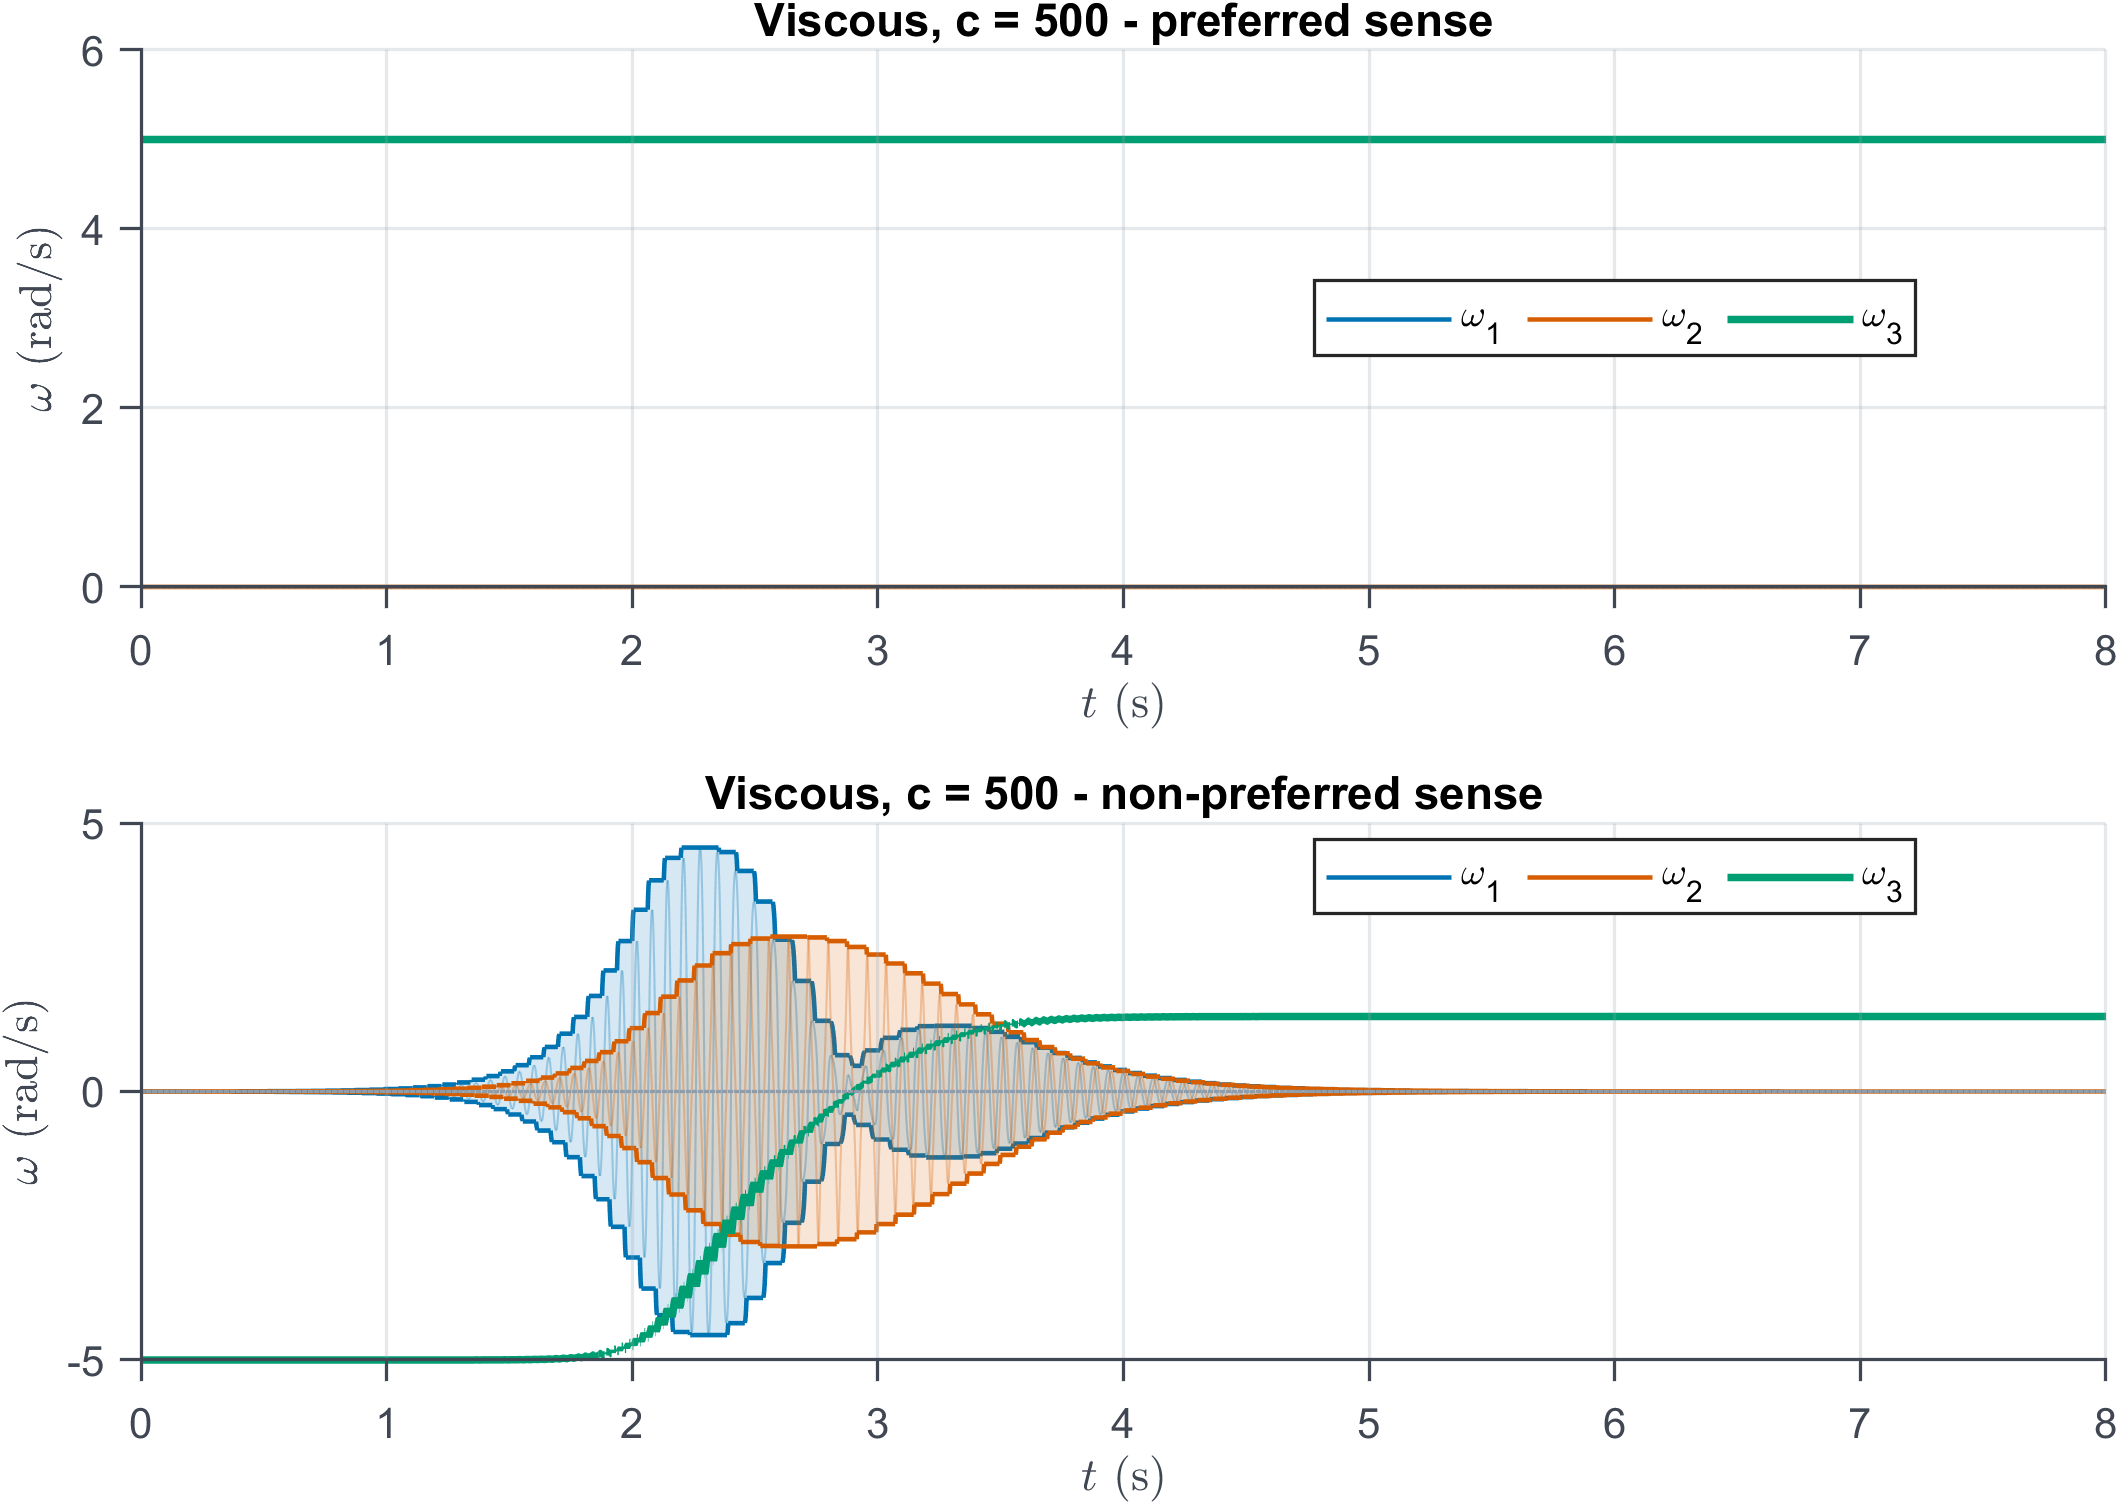
\includegraphics[width=\columnwidth]{figs/omega_viscous.png}\\[2pt]
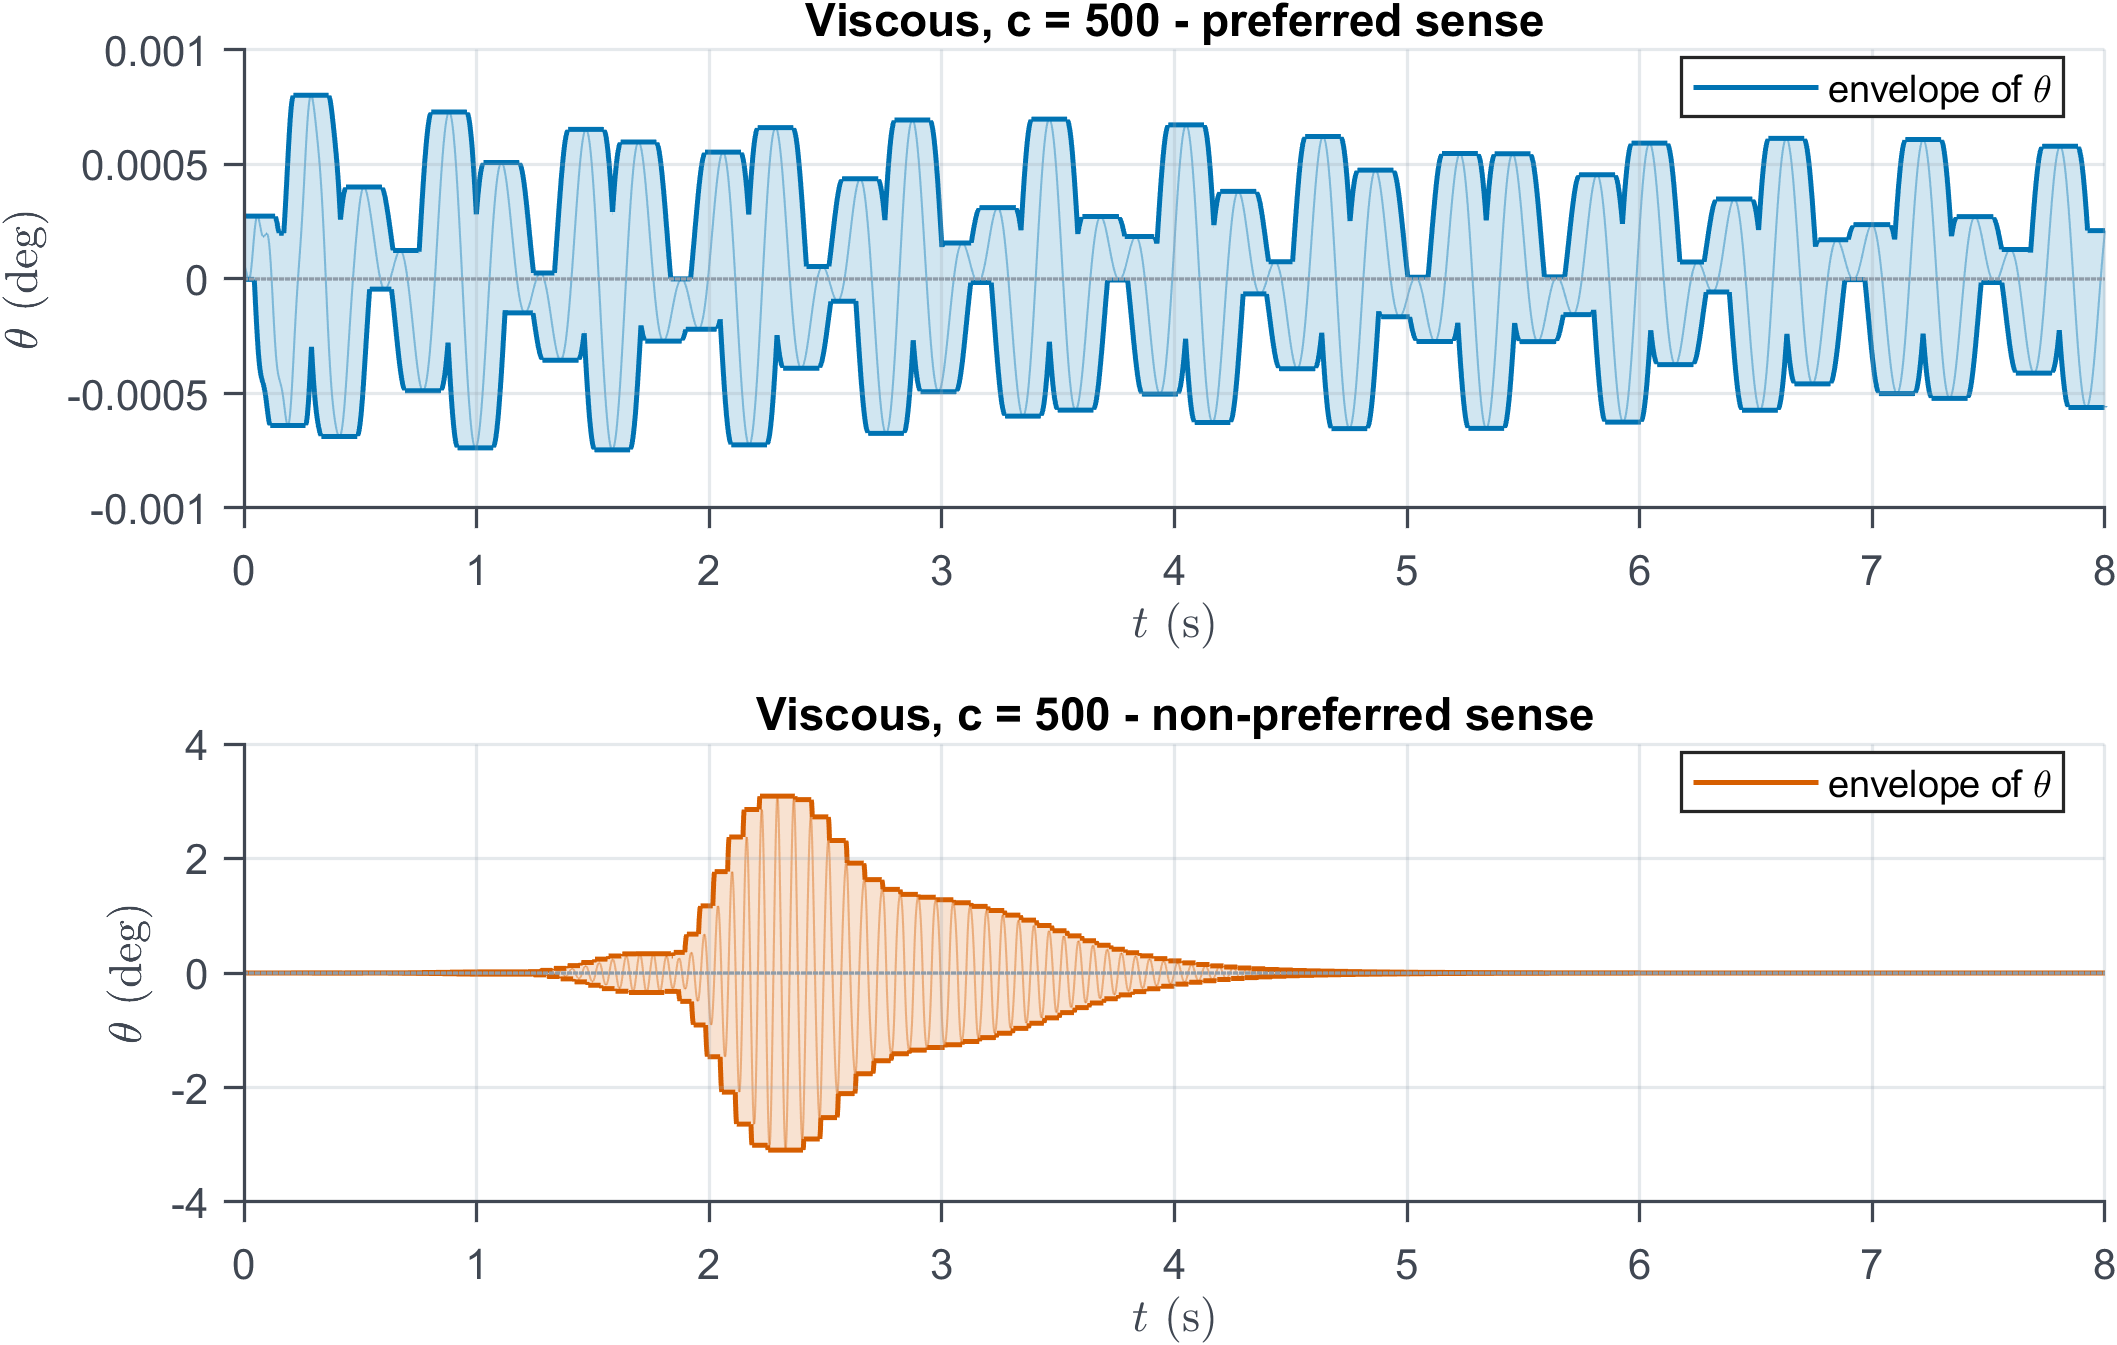
\includegraphics[width=\columnwidth]{figs/theta_viscous.png}
\caption{Viscous friction, $c_v=500$\,kg\,s$^{-1}$. Upper pair: angular velocity
components. Lower pair: rocking angle. The reversal occurs at $2.90$\,s, close to the
rolling value, with partial recovery of the spin to $+1.40$\,rad\,s$^{-1}$ and
$\theta_{\max}=3.09^\circ$.}
\label{fig:viscous}
\end{figure}

\begin{figure}[!tbp]
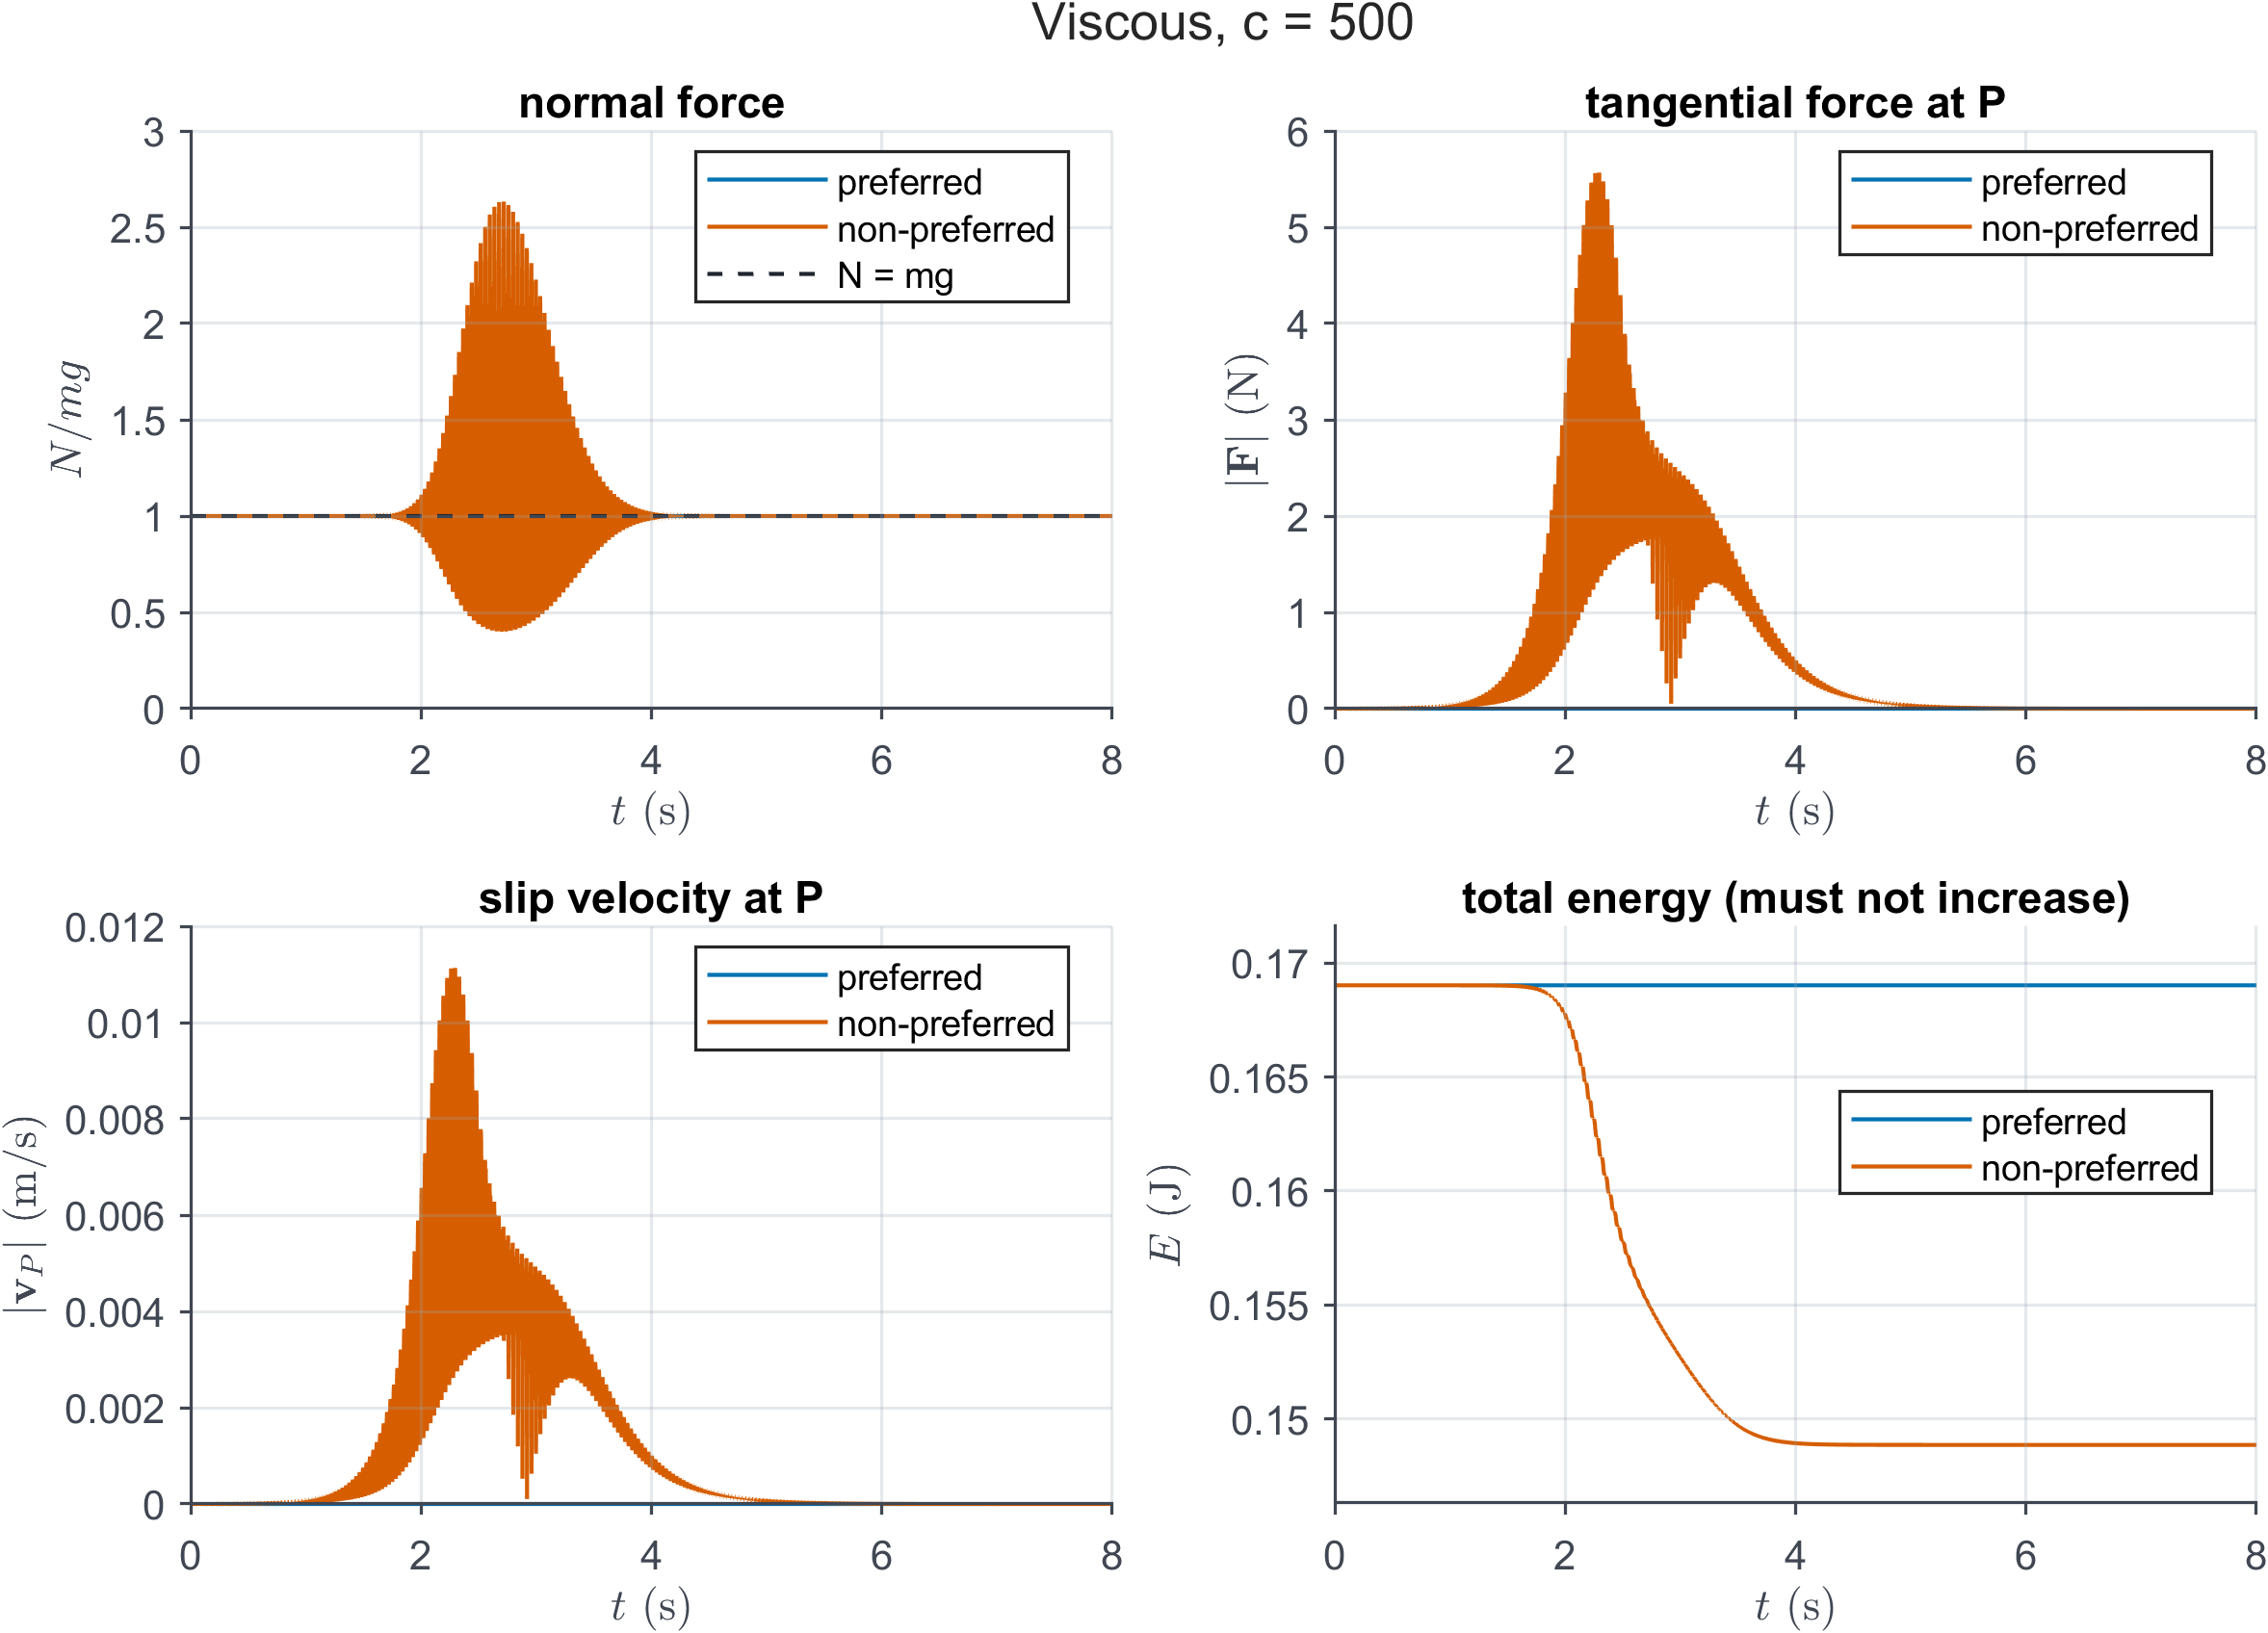
\includegraphics[width=\columnwidth]{figs/contact_viscous.png}
\caption{Contact diagnostics for viscous friction, $c_v=500$\,kg\,s$^{-1}$. The normal
reaction rises to $2.6\,mg$ and falls to $0.4\,mg$, a much larger excursion than with
Coulomb friction because the rocking is less strongly damped.}
\label{fig:contactviscous}
\end{figure}

\begin{table}[!tbp]
\caption{Viscous coefficient sweep, non-preferred sense. A dash denotes no reversal within
$8$\,s. The rolling reversal time is $2.83$\,s.}
\label{tab:viscous}
\begin{ruledtabular}
\begin{tabular}{lcccccc}
$c_v$ (kg\,s$^{-1}$) & 1.5 & 10 & 50 & 200 & 500 & 2000 \\
\hline
$t_{\rm rev}$ (s) & -- & -- & -- & -- & 2.90 & 2.81 \\
$\omega_3(8\,{\rm s})$ & $-5.00$ & $-5.00$ & $-4.78$ & $-0.34$ & $+1.40$ & $+3.62$ \\
\end{tabular}
\end{ruledtabular}
\end{table}

With $c_v=500$\,kg\,s$^{-1}$ (Figs.~\ref{fig:viscous} and \ref{fig:contactviscous}) the
viscous model reverses at $2.90$\,s, close to rolling, and retains more of its spin than
the Coulomb model. The structural difference between the two laws is exposed by a sweep
in $c_v$ (Table~\ref{tab:viscous}). A coefficient of the same nominal size as the Coulomb
case, $c_v=\mu mg/(1\,{\rm m\,s^{-1}})\approx1.5$\,kg\,s$^{-1}$, produces a tangential
force of order $10^{-2}$\,N at the observed slip speeds. The contact is then effectively
frictionless, the rocking modes are not excited, and the spin remains at
$-5$\,rad\,s$^{-1}$; the same holds for $c_v=10$\,kg\,s$^{-1}$. At
$c_v=50$\,kg\,s$^{-1}$ the spin begins to decrease, and at $200$\,kg\,s$^{-1}$ it reaches
$-0.34$\,rad\,s$^{-1}$ by $t=8$\,s without reversing. Reversal requires
$c_v\gtrsim500$\,kg\,s$^{-1}$, and at $2000$\,kg\,s$^{-1}$ the reversal time, $2.81$\,s,
is close to the rolling value. In this regime the viscous law acts as a penalty that
enforces approximate rolling.

The contrast follows from the property noted after Eq.~\eqref{eq:viscous}. The
instability needs a tangential force large enough to couple the rocking modes to the
spin. A Coulomb contact supplies a force of order $\mu N$ however small the slip, whereas
a viscous contact supplies one only if $c_v$ is large compared with $N$ divided by a
typical slip speed. In the gyroscopic-balance analysis of Ref.~\cite{Moffatt2002} the same
distinction separates a transition completed in finite time [their Eq.~(15)] from an
exponential approach [their Eq.~(16)]. In the rattleback it decides whether a reversal
occurs at all.

\subsection{Drilling friction}\label{sec:spinresult}

\begin{figure}[!tbp]
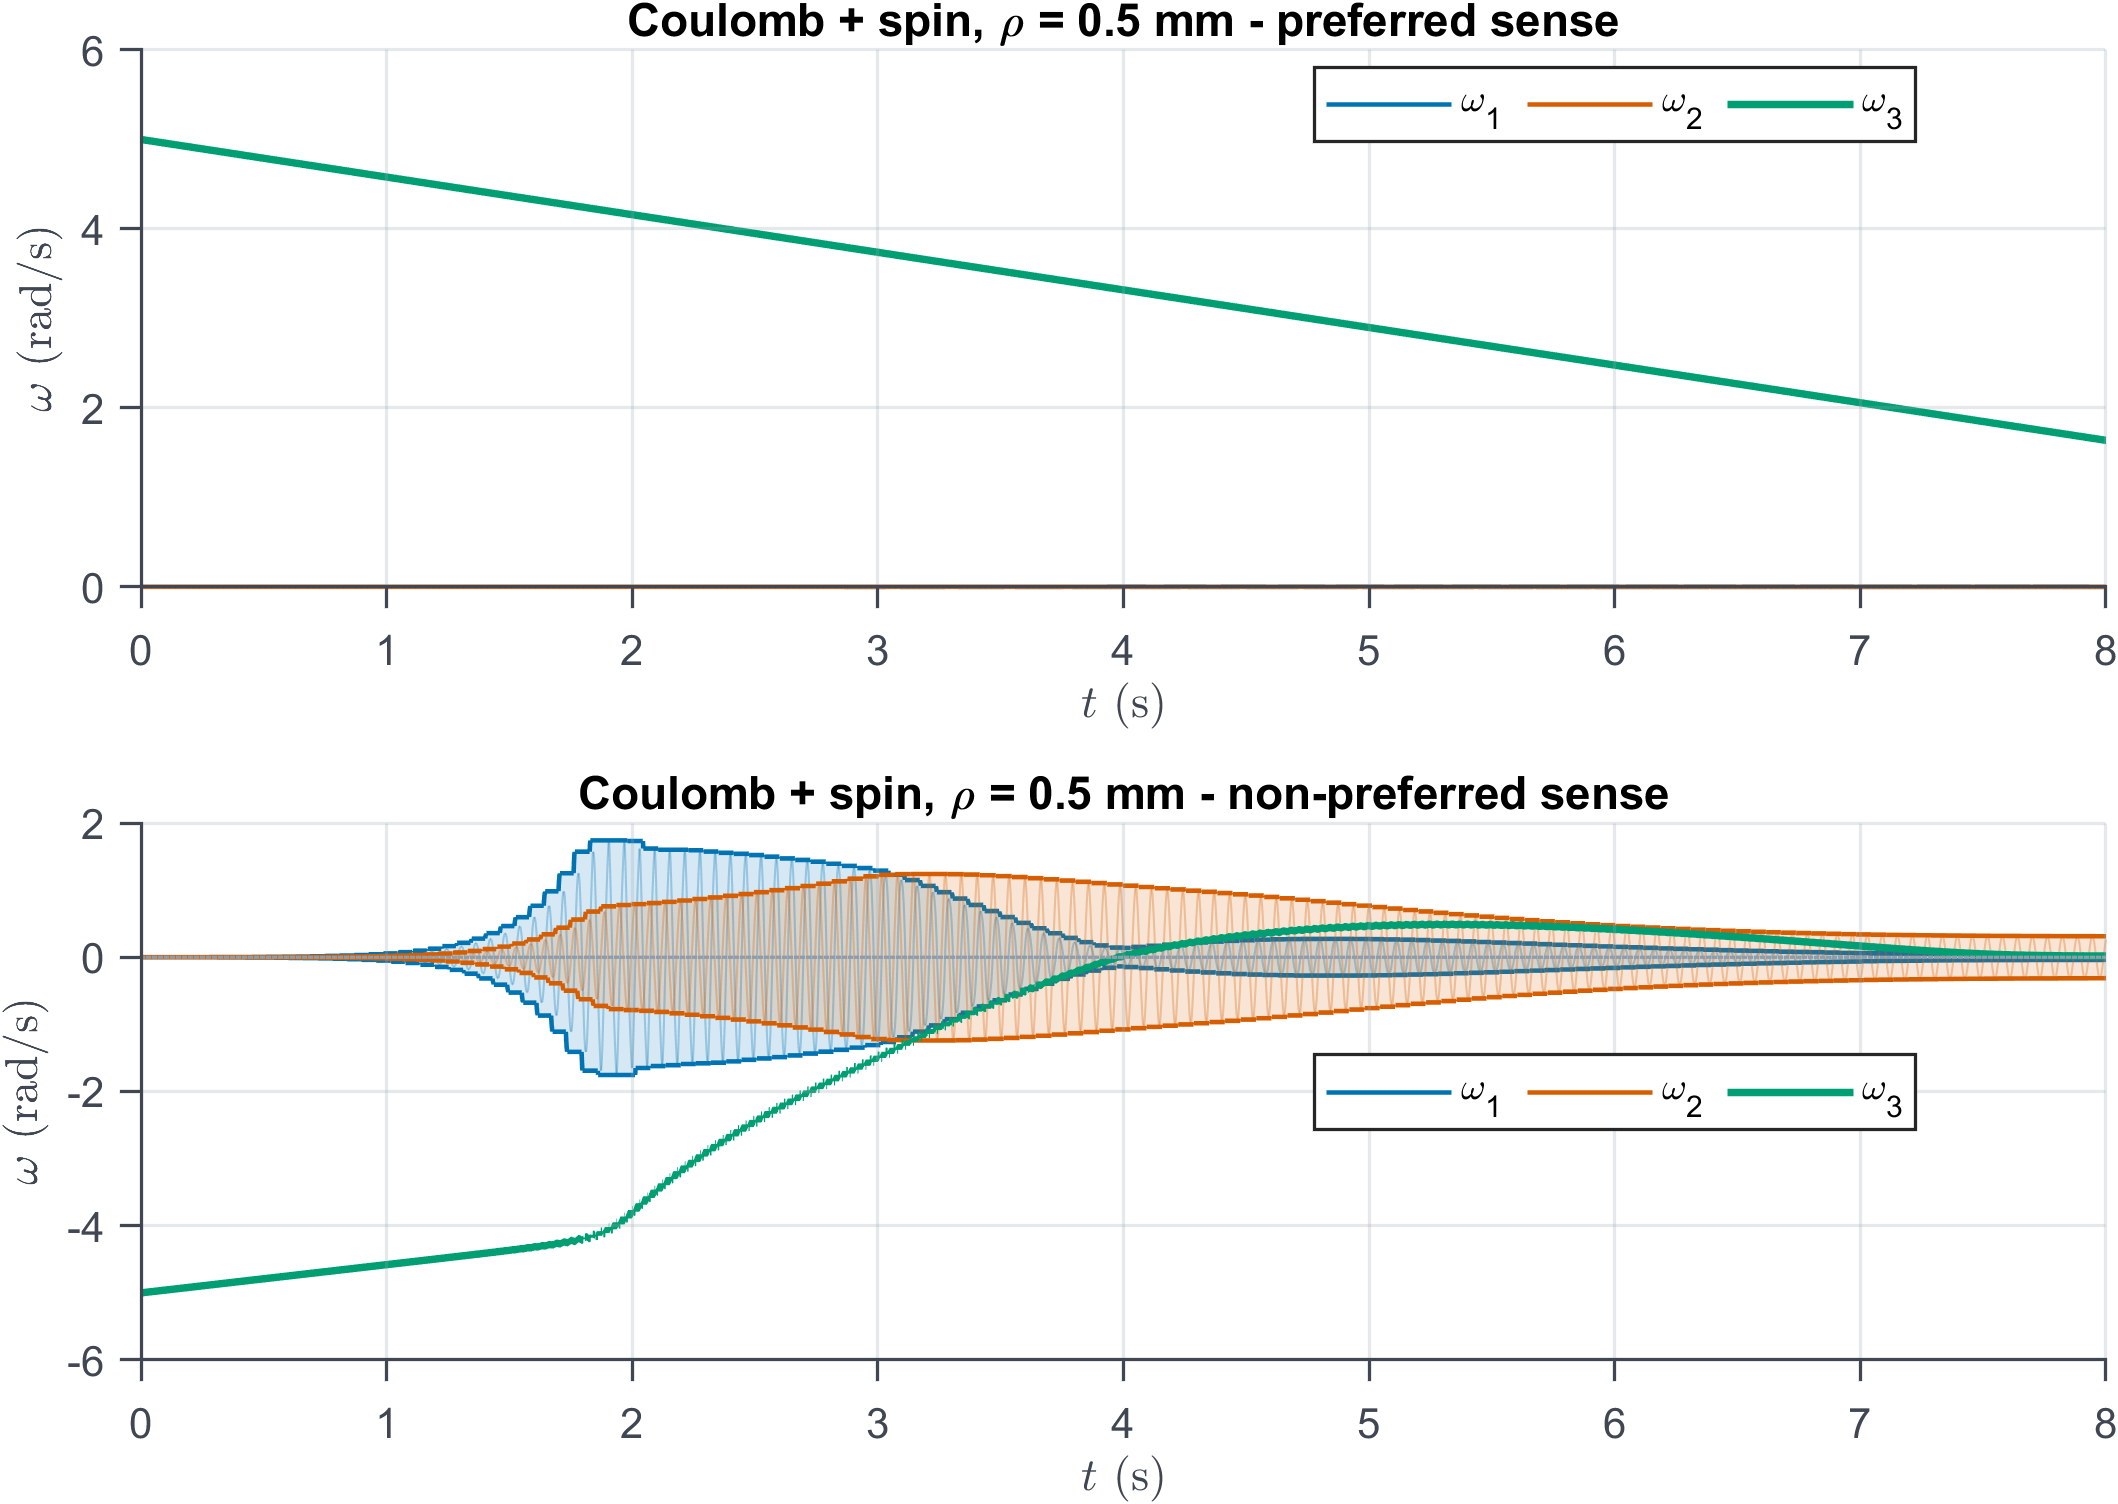
\includegraphics[width=\columnwidth]{figs/omega_coulomb_spin.png}\\[2pt]
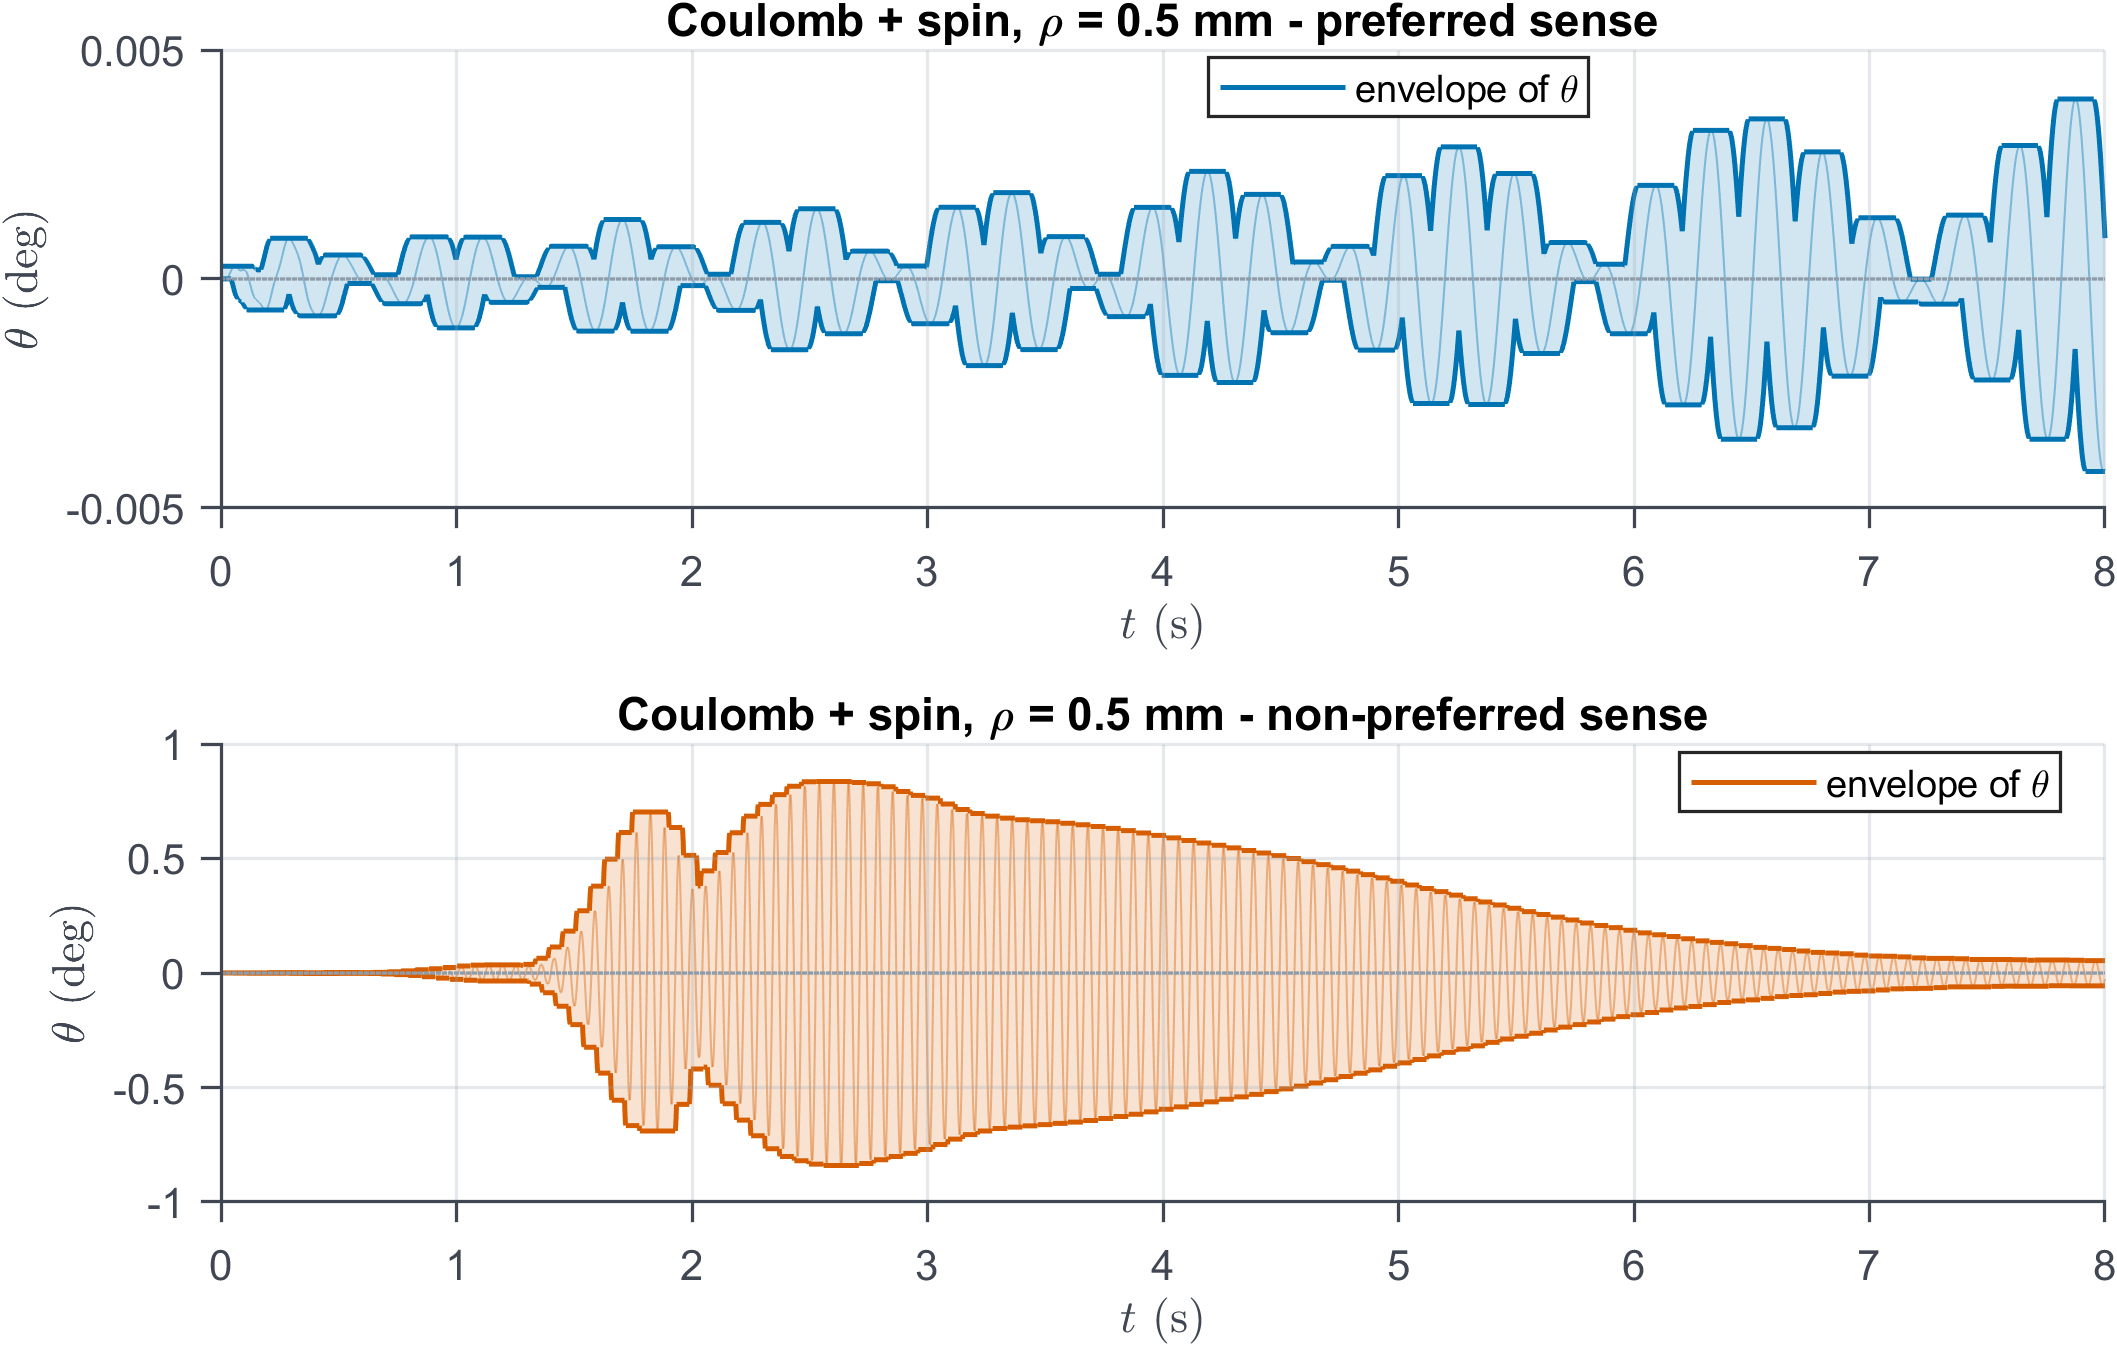
\includegraphics[width=\columnwidth]{figs/theta_coulomb_spin.png}
\caption{Coulomb friction ($\mu=0.15$) with a drilling torque, $\rho=0.5$\,mm. Upper
pair: angular velocity components. Lower pair: rocking angle. In the non-preferred sense
the reversal occurs at $3.98$\,s with the rocking unchanged at $0.84^\circ$, after which
the drilling torque brings the spin nearly to rest. In the preferred sense the spin
decays steadily from $5$ to $1.64$\,rad\,s$^{-1}$.}
\label{fig:spin}
\end{figure}

\begin{figure}[!tbp]
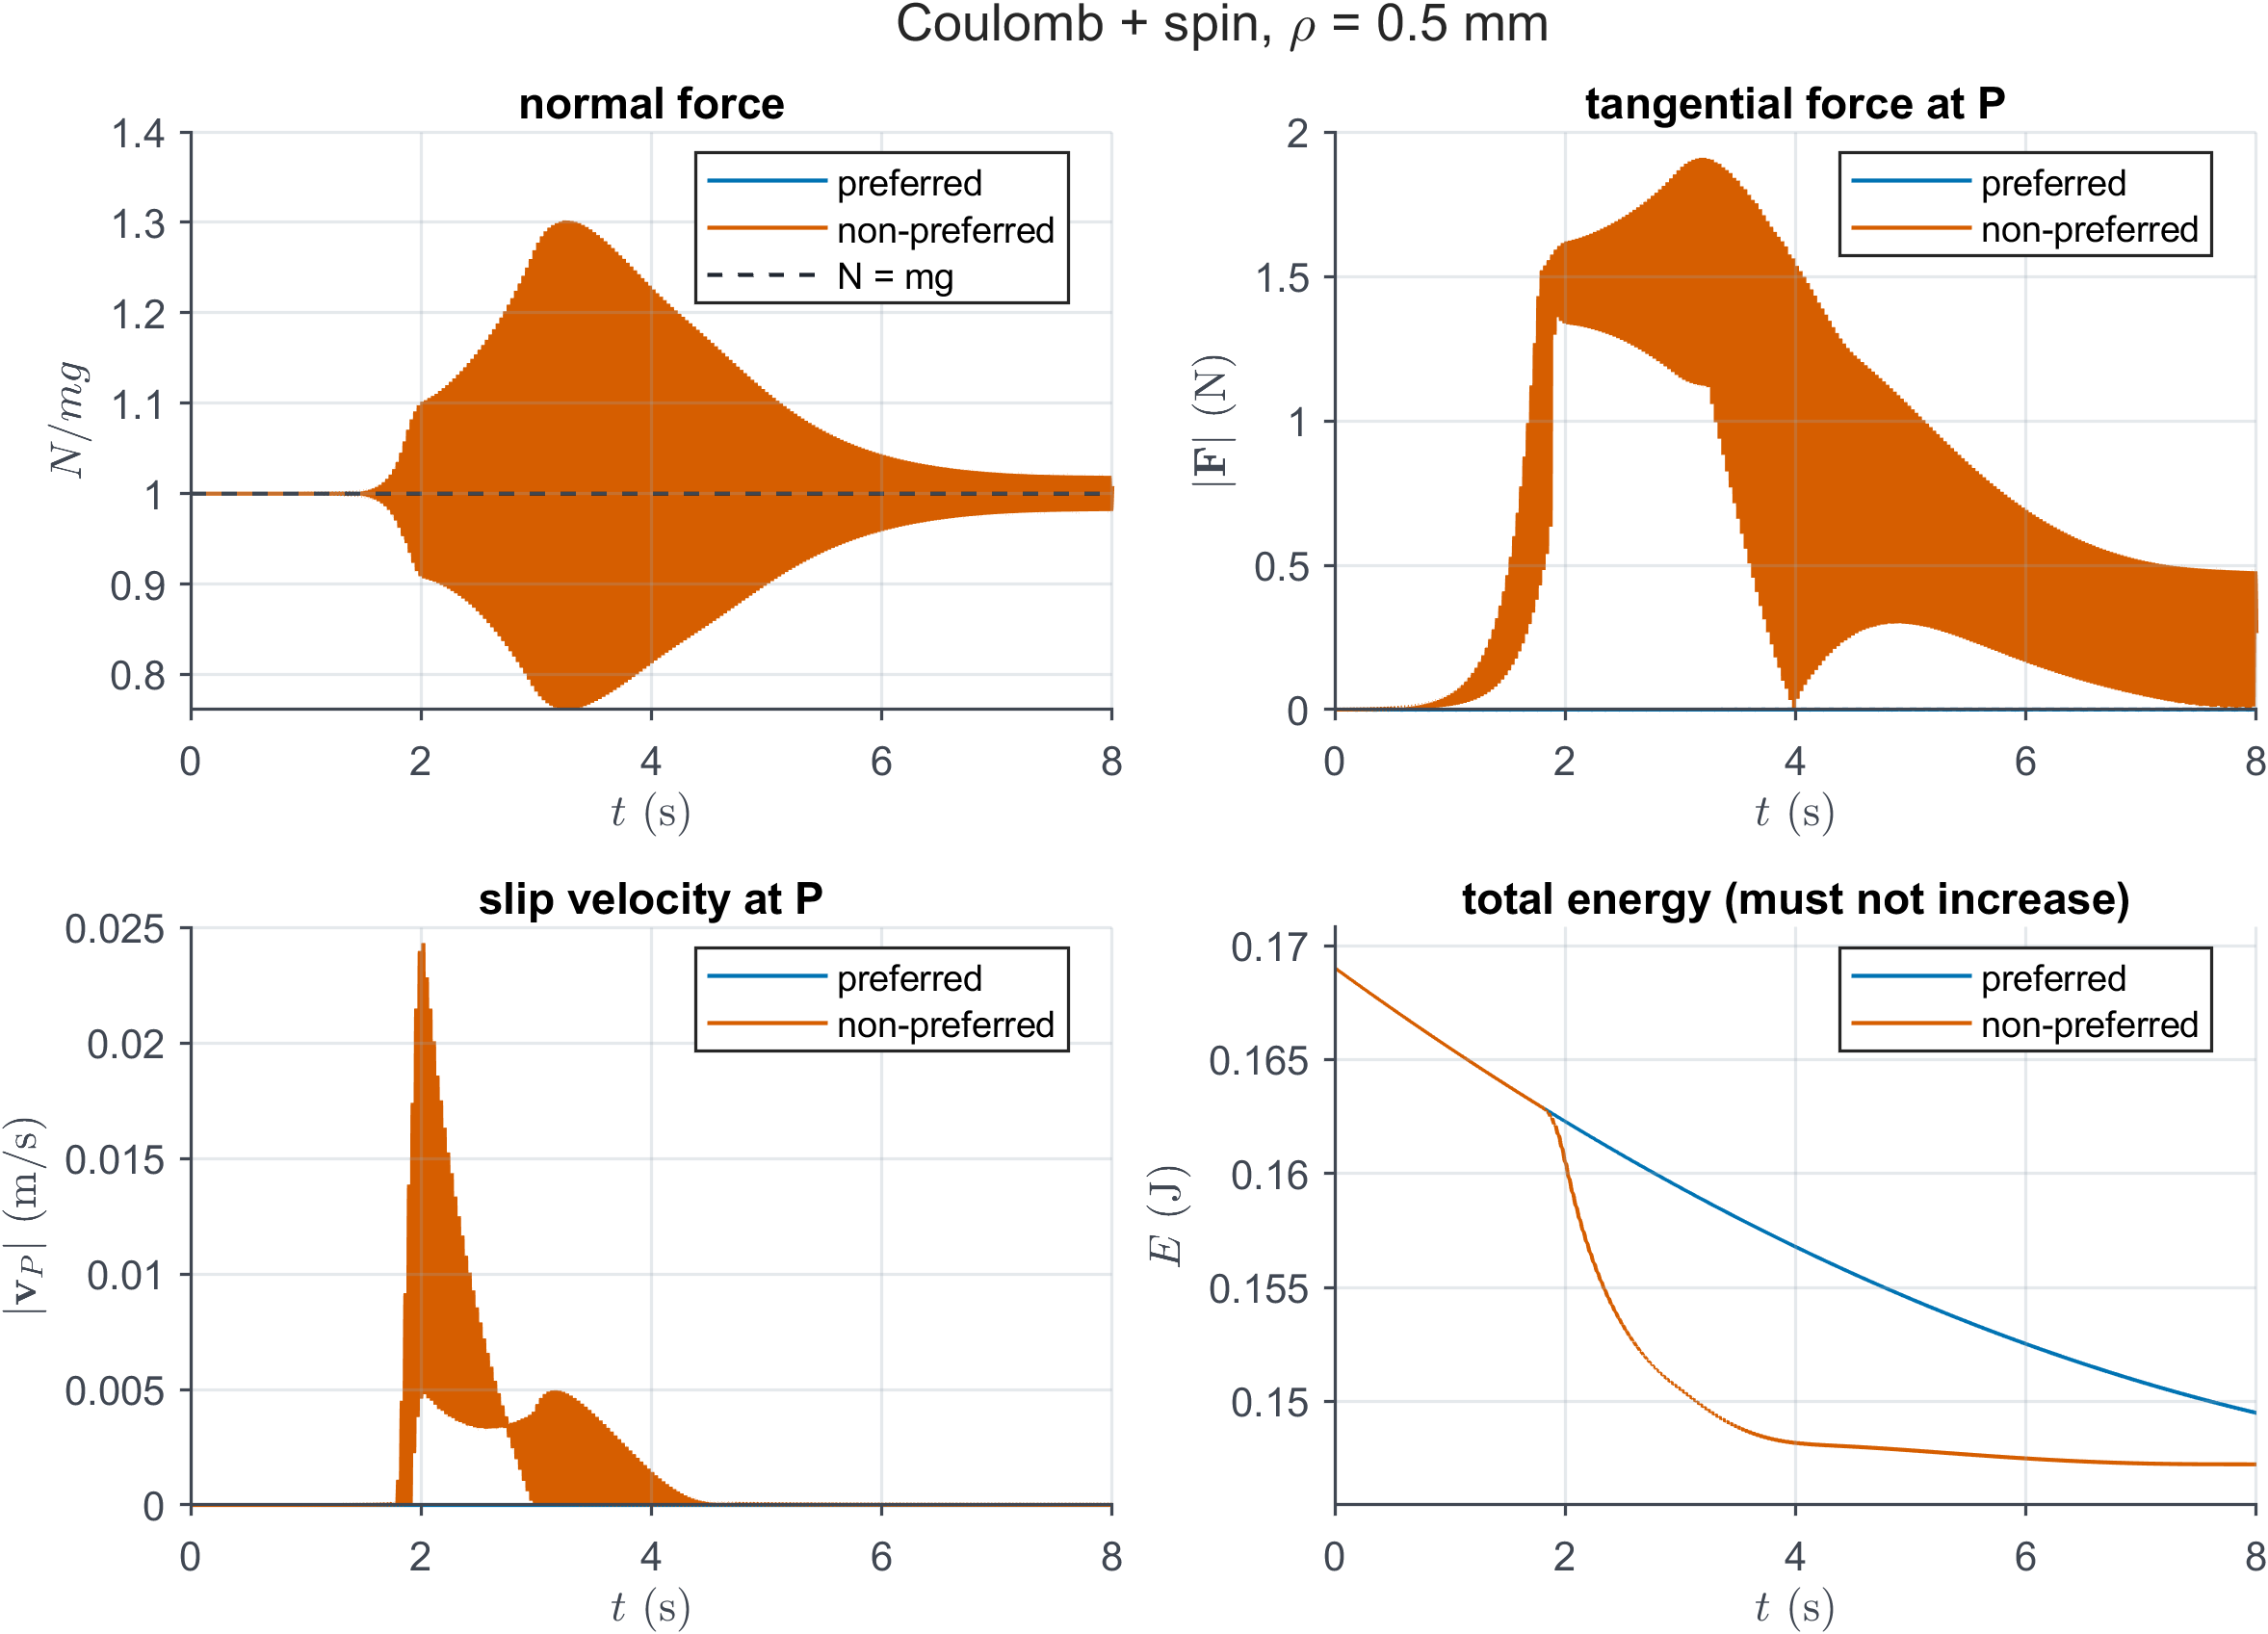
\includegraphics[width=\columnwidth]{figs/contact_coulomb_spin.png}
\caption{Contact diagnostics for Coulomb friction with drilling torque, $\rho=0.5$\,mm.
Unlike the other models, the energy decreases in the preferred sense as well, because the
drilling torque acts on the spin directly.}
\label{fig:contactspin}
\end{figure}

\begin{table}[!tbp]
\caption{Contact patch sweep for Coulomb friction with drilling torque, $\mu=0.15$.
$t_\times$ is the first zero crossing of $\omega_3$ in the non-preferred sense; at
$\rho=2$\,mm it is a spin-down rather than a reversal. The Hertzian estimate is
$\rho\approx0.16$--$0.52$\,mm.}
\label{tab:spin}
\begin{ruledtabular}
\begin{tabular}{lcccccc}
$\rho$ (mm) & 0 & 0.1 & 0.2 & 0.5 & 1.0 & 2.0 \\
\hline
$t_\times$ (s) & 4.22 & 4.19 & 4.15 & 3.98 & 3.68 & 2.99 \\
$\omega_3(8\,{\rm s})$, pref. & 5.00 & 4.33 & 3.66 & 1.64 & 0.00 & 0.00 \\
$\omega_3(8\,{\rm s})$, non-pref. & 1.01 & 0.78 & 0.52 & 0.02 & 0.02 & 0.00 \\
$\theta_{\max}$ (deg) & 0.84 & 0.84 & 0.84 & 0.84 & 0.72 & 0.06 \\
\end{tabular}
\end{ruledtabular}
\end{table}

\begin{figure}[!tbp]
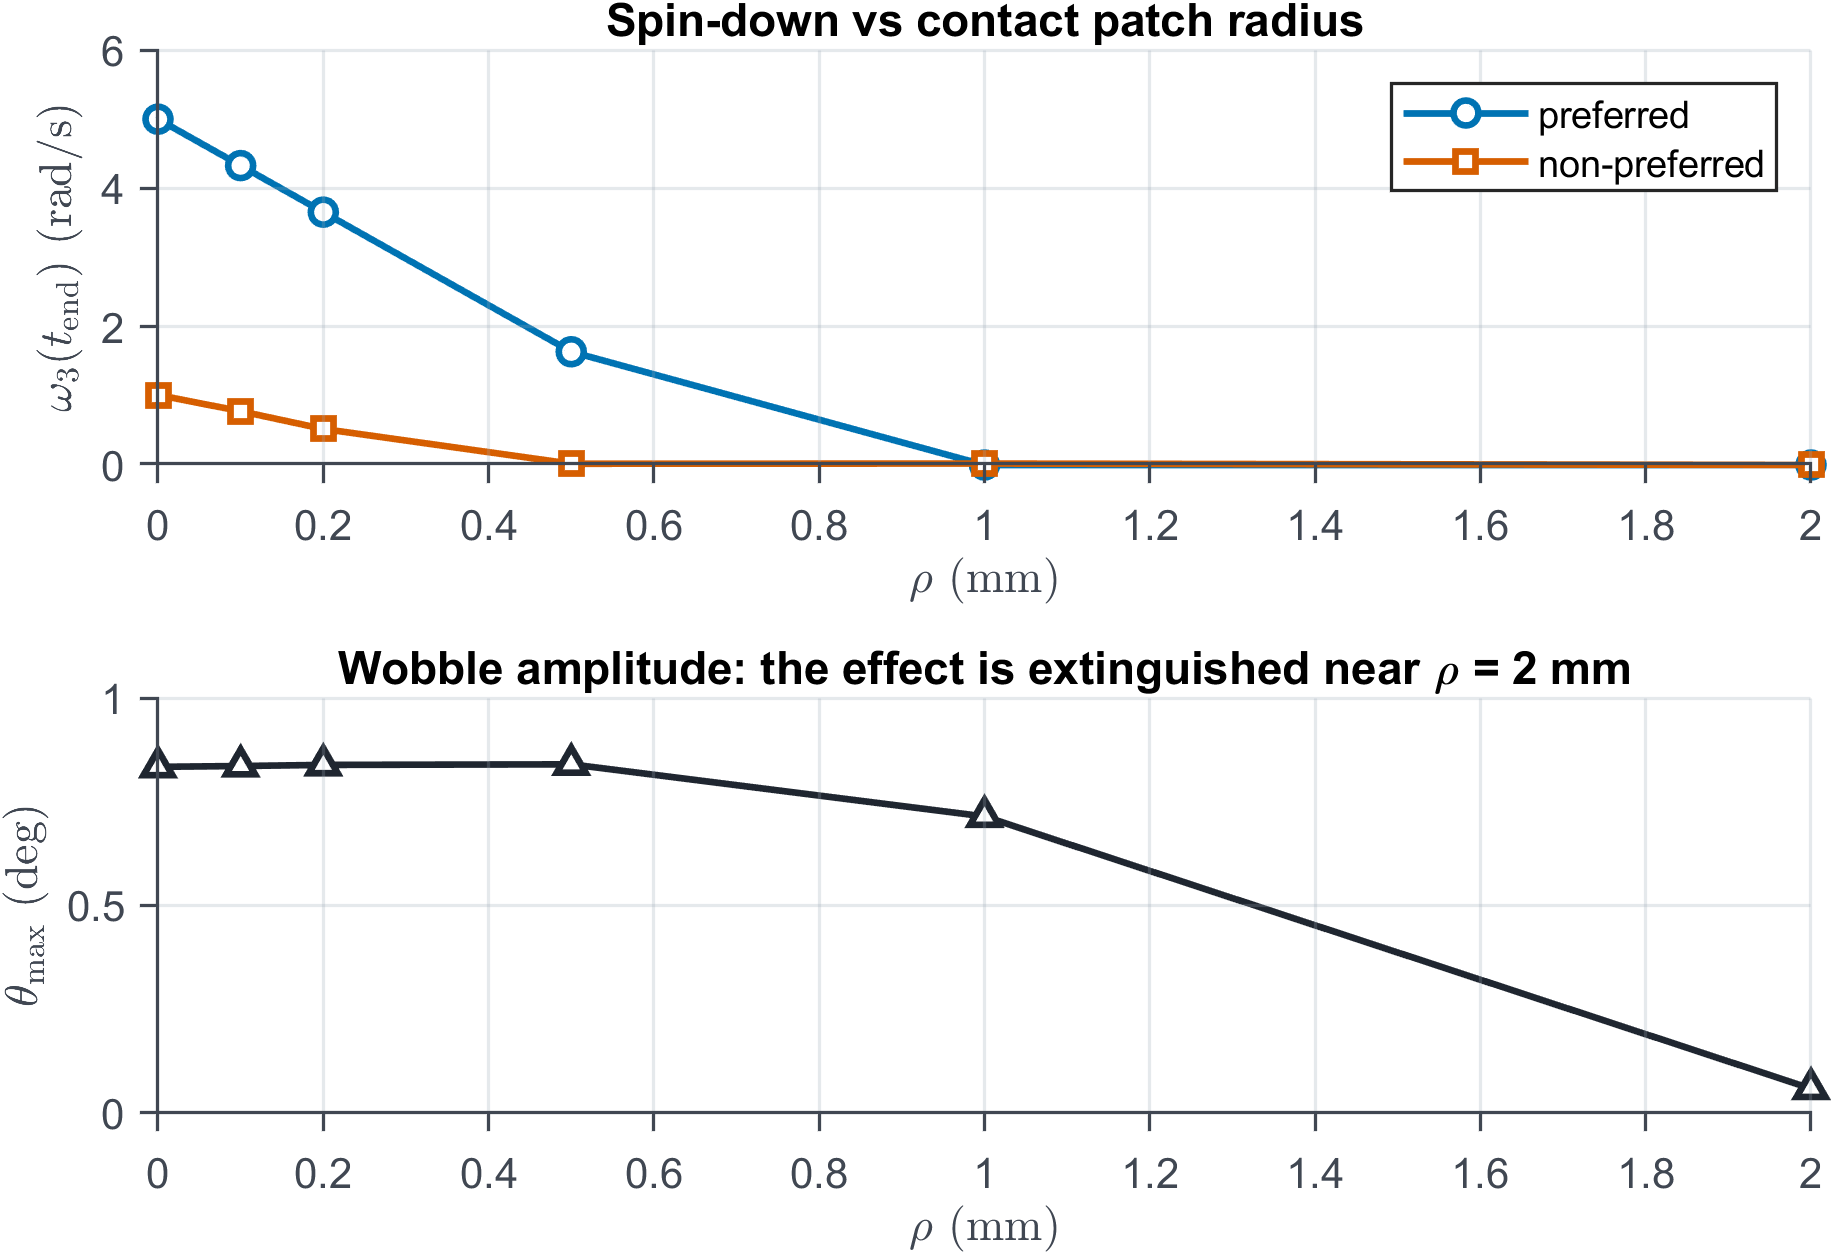
\includegraphics[width=\columnwidth]{figs/sweep_rho.png}
\caption{Effect of the drilling lever arm $\rho$, Coulomb friction with $\mu=0.15$. Top:
spin at $t=8$\,s in both senses. Bottom: maximum rocking angle in the non-preferred
sense.}
\label{fig:rho}
\end{figure}

Drilling friction removes energy from the spin directly, without involving the rocking
modes. At the representative lever arm $\rho=0.5$\,mm (Figs.~\ref{fig:spin} and
\ref{fig:contactspin}) the rocking amplitude is unchanged at $0.84^\circ$ and the reversal
still occurs, slightly earlier, at $3.98$\,s, because the spin to be reversed has already
been partly braked. The torque continues to act after the reversal, and the spin at
$t=8$\,s is only $0.02$\,rad\,s$^{-1}$. In the preferred sense, where no rocking develops,
drilling friction is the only dissipation, and the spin decays from $5$ to
$1.64$\,rad\,s$^{-1}$ in $8$\,s. A slow spin-down in the preferred sense is the expected
behavior of a real celt and corrects a shortcoming of the conservative rolling model, in
which the preferred spin persists indefinitely.

The sweep in $\rho$ (Table~\ref{tab:spin}, Fig.~\ref{fig:rho}) shows how sensitive the
effect is to the assumed patch size. Within the Hertzian range the rocking survives
essentially unchanged. For larger patches the drilling torque dominates. At $\rho=2$\,mm
the torque $\mu N\rho\approx2.9$\,mN\,m, acting against $I_{33}=1.75\times10^{-3}$\,kg\,m$^2$,
decelerates the spin at about $1.7$\,rad\,s$^{-2}$ and brings $5$\,rad\,s$^{-1}$ to rest in
about $3$\,s. This happens before the instability can grow, and the maximum rocking angle
falls to $0.06^\circ$. The zero crossing of $\omega_3$ at $2.99$\,s is then a spin-down,
not a reversal: the spin approaches zero and does not recover. This is a property of the
model rather than a numerical artifact. A reversal requires the growth time of the
instability to be shorter than the spin-down time set by drilling friction, and an
oversized patch violates that condition.

\subsection{The normal reaction}\label{sec:normalresults}

\begin{figure*}[!tbp]
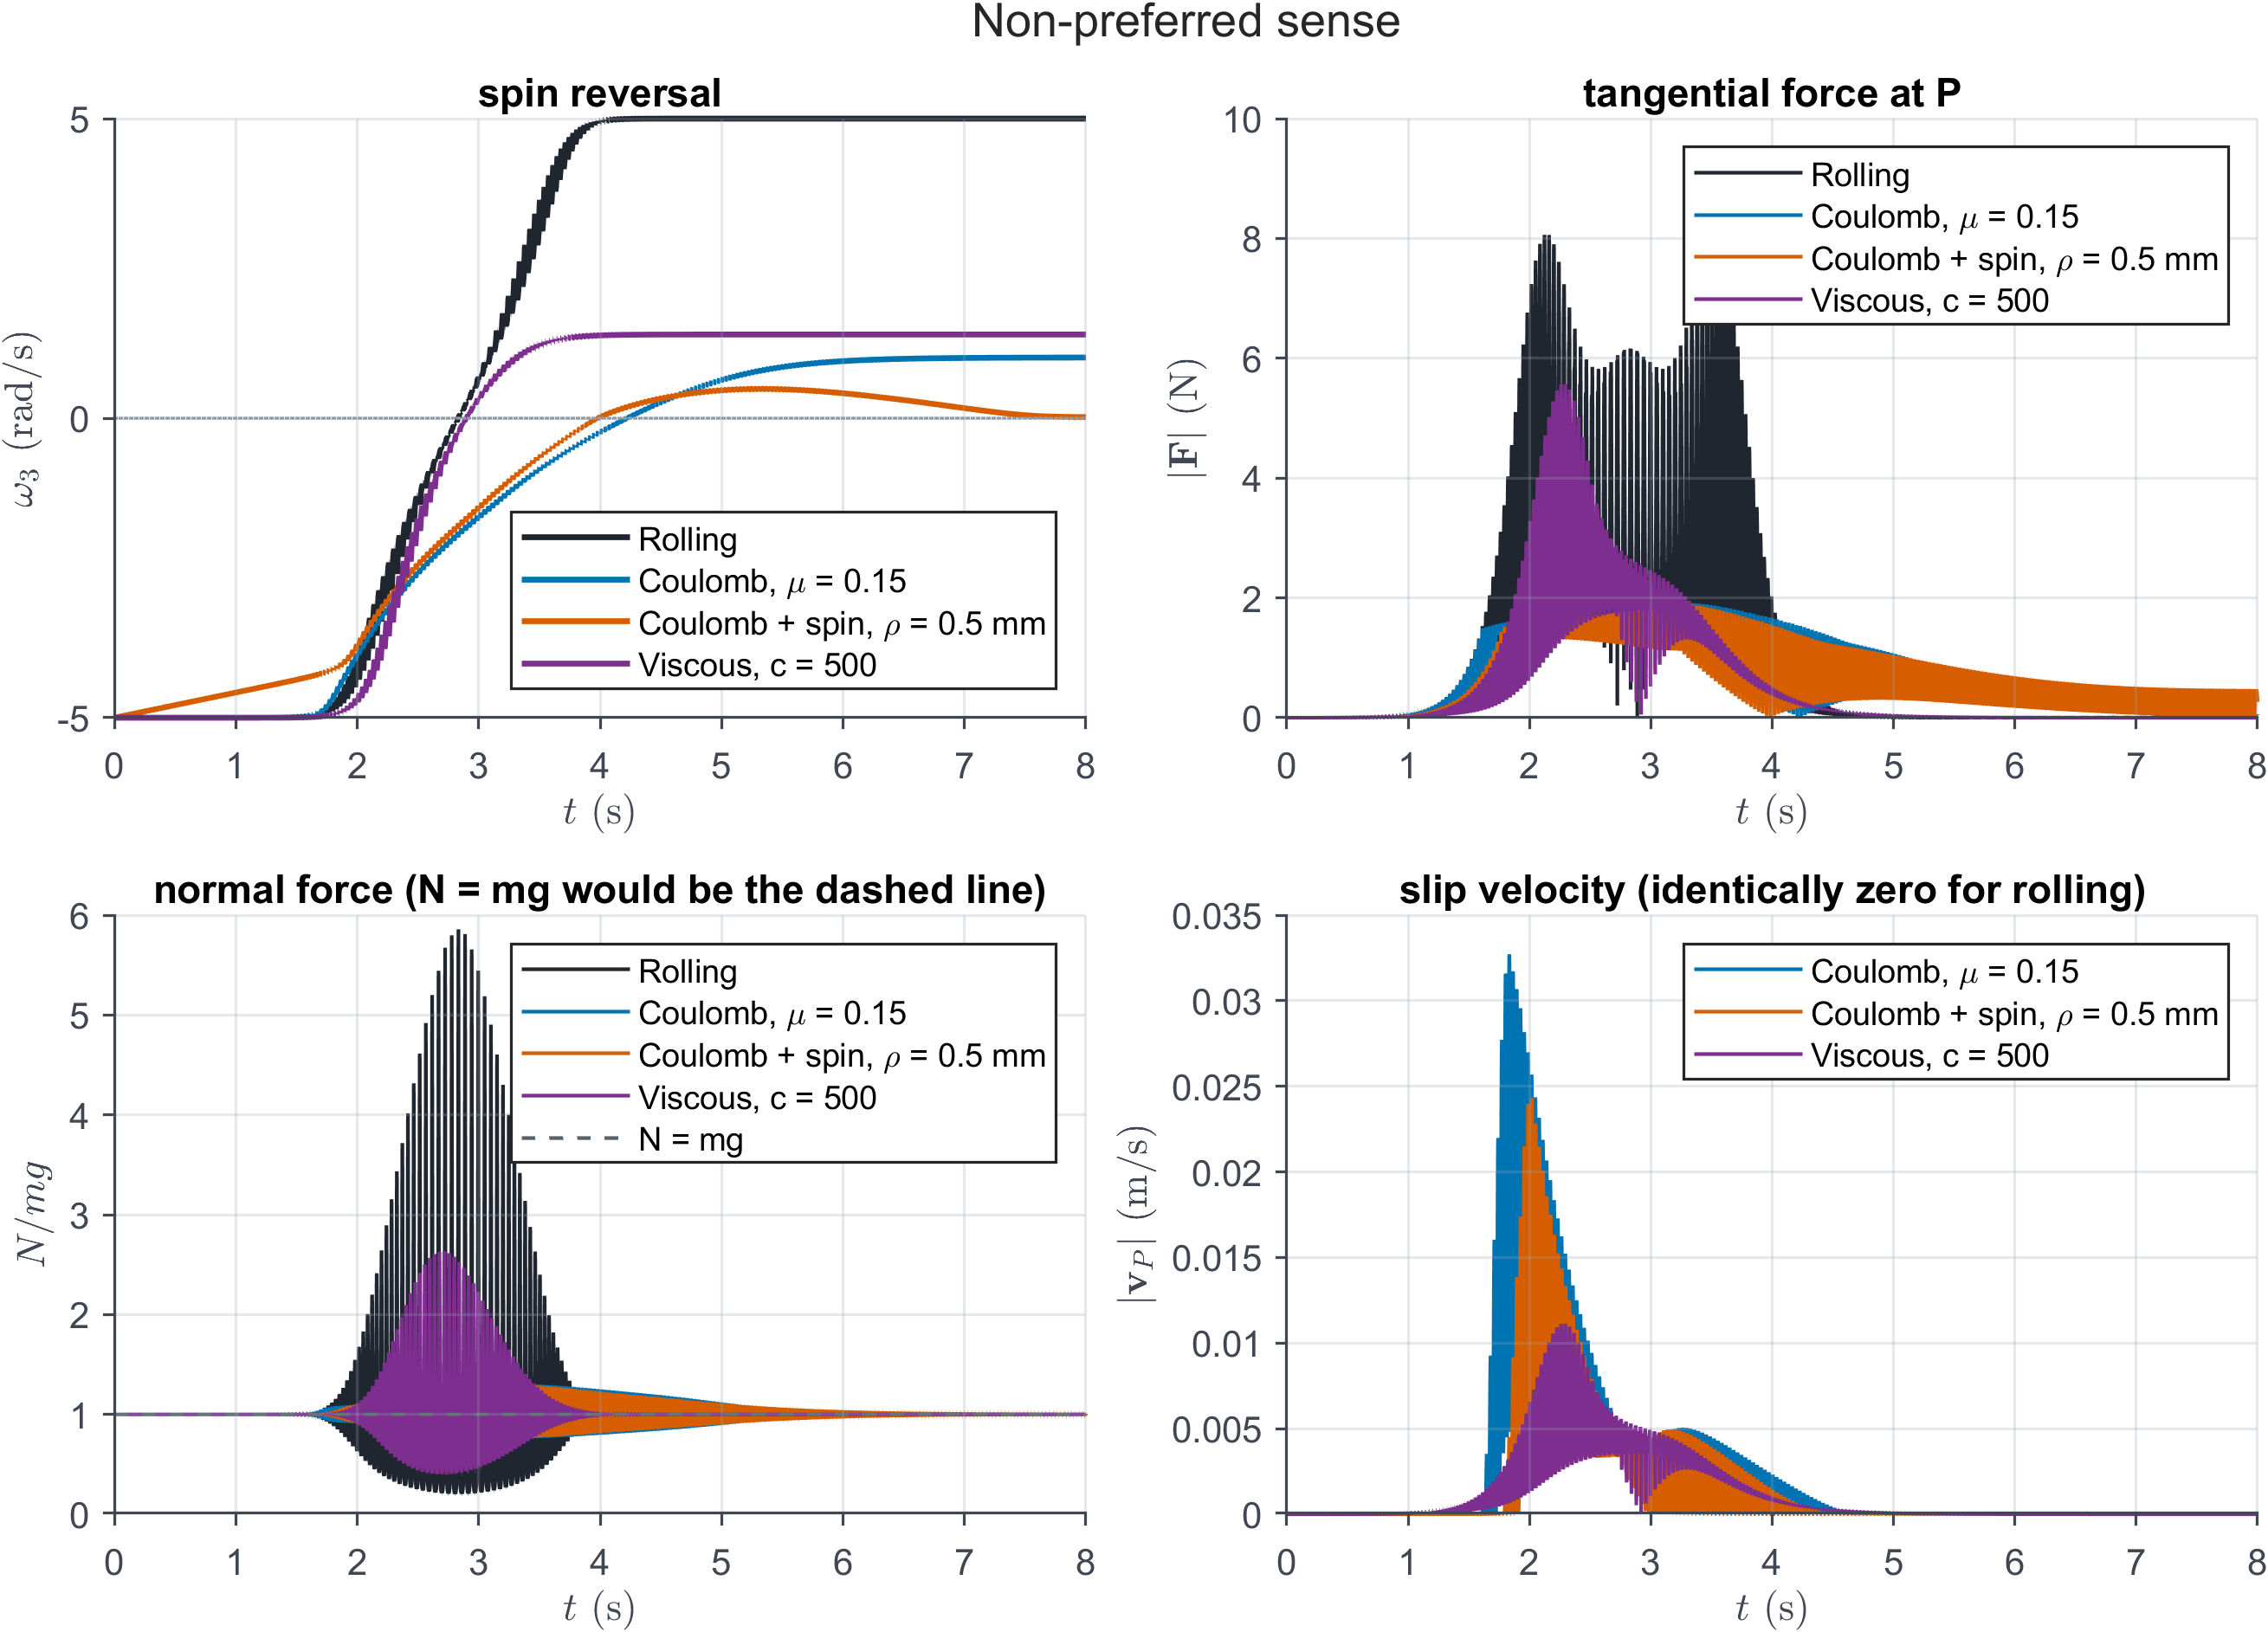
\includegraphics[width=0.92\textwidth]{figs/comparison_contact.png}
\caption{Comparison of the four contact models in the non-preferred sense. Top left: spin
$\omega_3$. Top right: magnitude of the tangential force. Bottom left: normal reaction
relative to $mg$; for the rolling solution it is the reaction required to sustain
rolling and spans $0.20\,mg$ to $5.86\,mg$. Bottom right: slip speed, zero for rolling by
definition.}
\label{fig:comparison}
\end{figure*}

The bottom-left panel of Fig.~\ref{fig:comparison} is the quantitative justification for
solving Eq.~\eqref{eq:N}. In the rolling solution, the exact no-slip motion, the normal
reaction oscillates at the rocking frequency of about $11$\,Hz and spans $0.20\,mg$ to
$5.86\,mg$, a factor of $29$. The tangential force needed to prevent slip reaches
$|\ve F|/N=0.79$ near $t=2.8$\,s, so pure rolling requires a friction coefficient of at
least about $0.8$ for these parameters. Kondo and Nakanishi found a maximum ratio of
about $0.2$ in the cases they examined \cite{Kondo2017}; the ratio depends strongly on the
rocking amplitude, which is large here. Even with Coulomb friction at $\mu=0.15$, where
the rocking is weak, the reaction departs from $mg$ by up to $30\%$. The assumption
$N=mg$ is therefore untenable during the rocking phase.

\begin{figure}[!tbp]
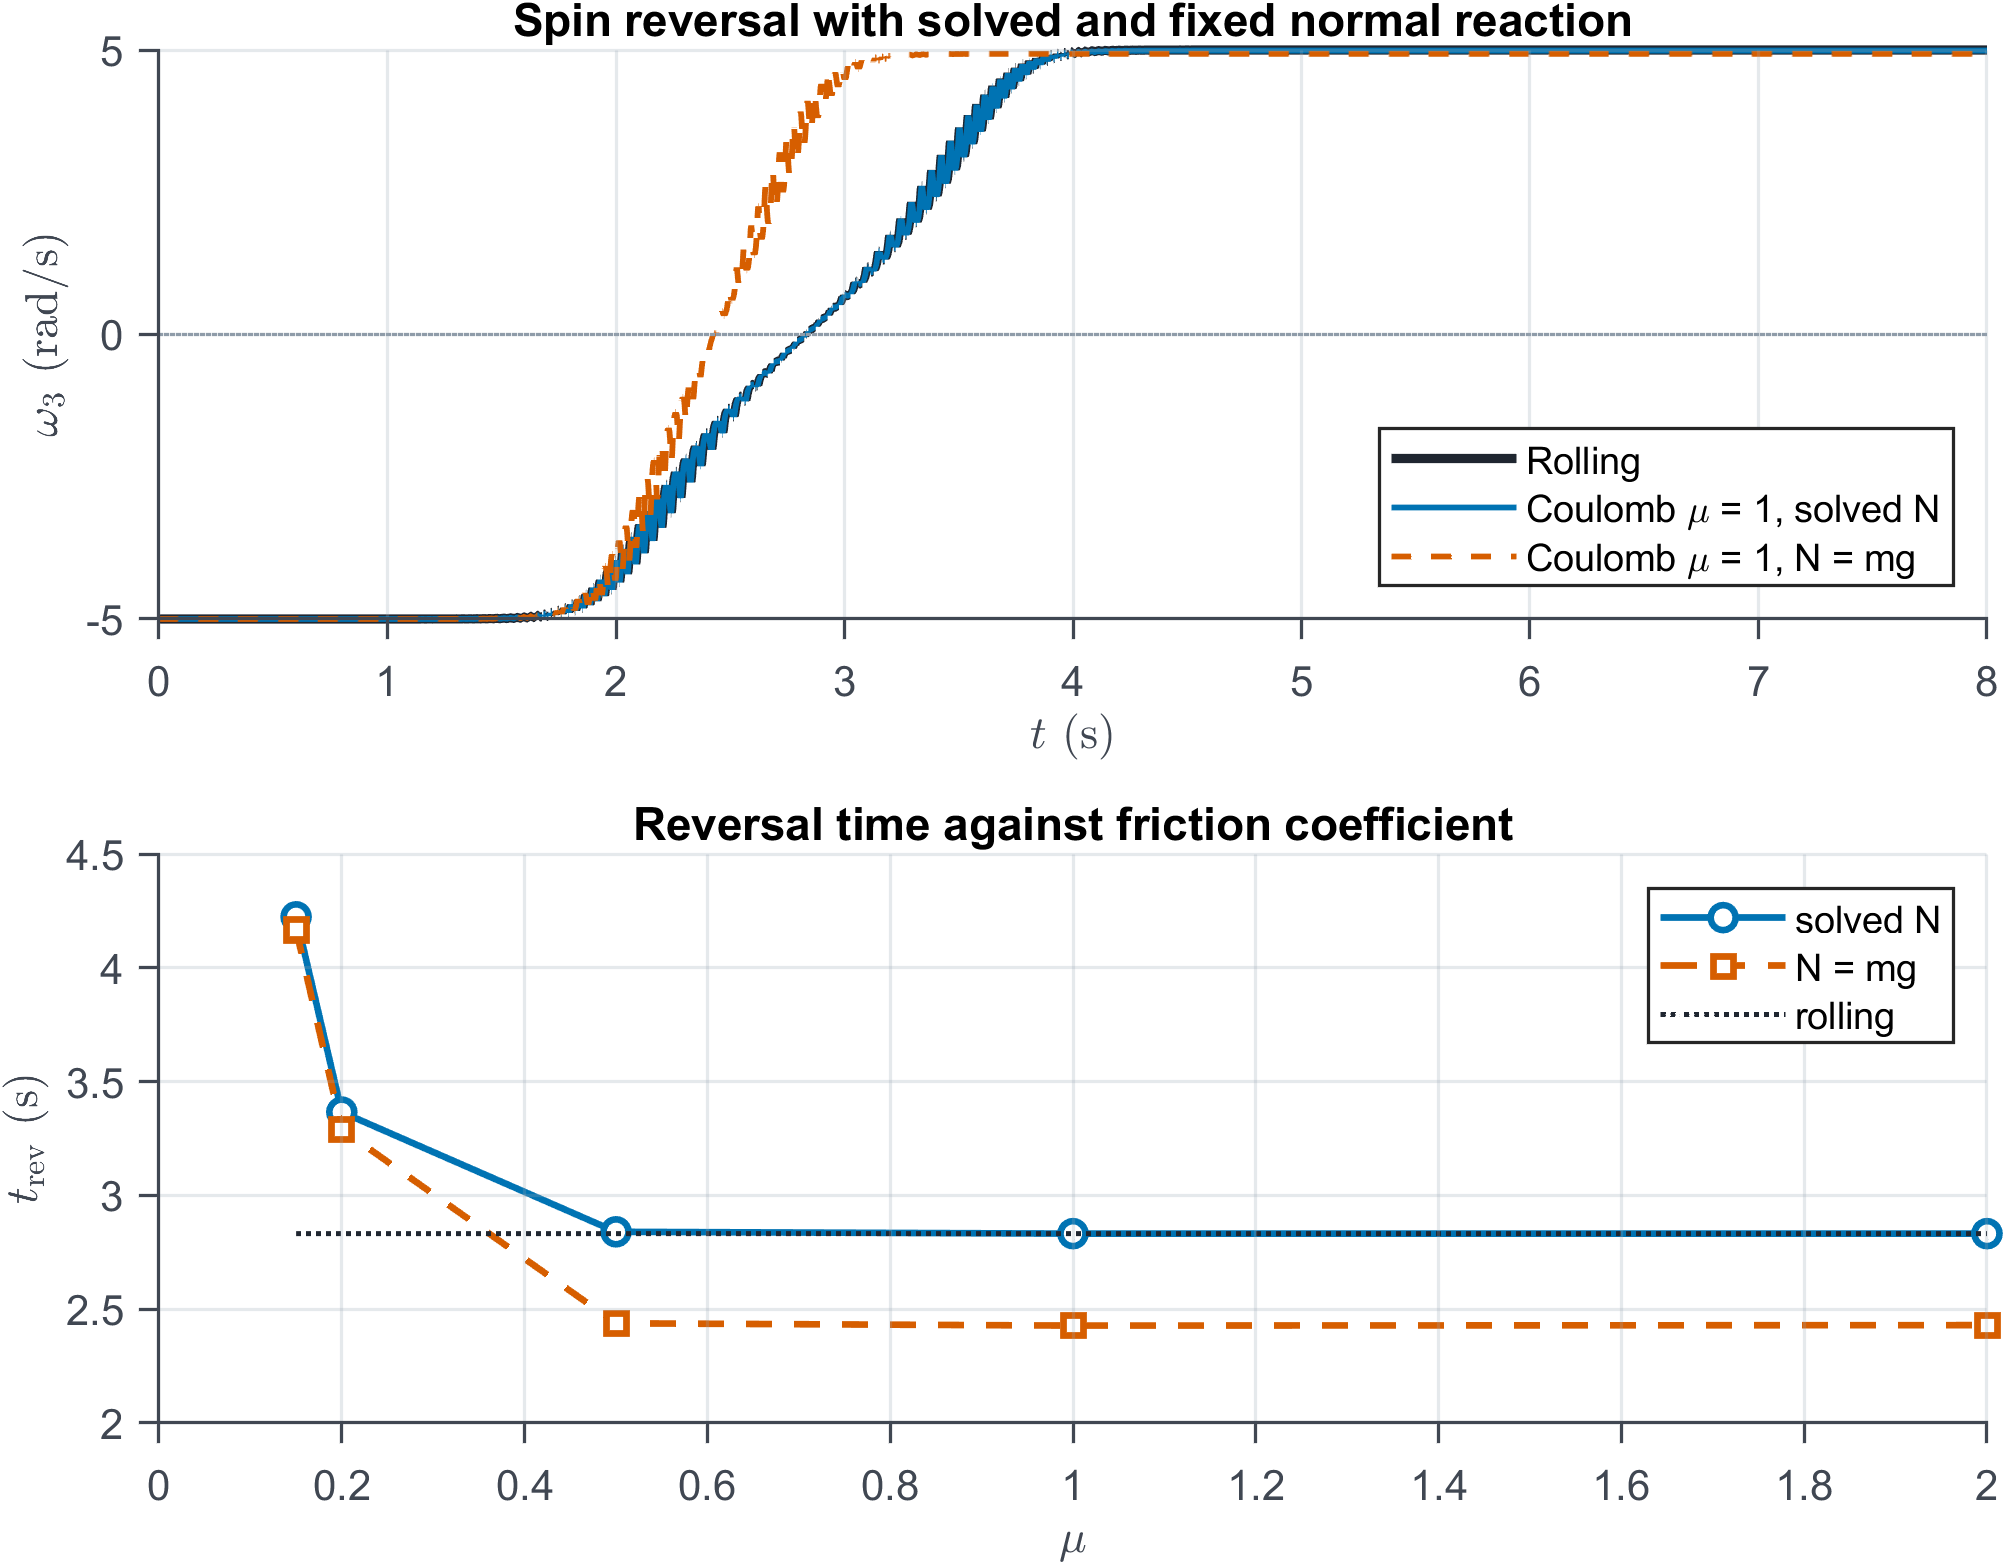
\includegraphics[width=\columnwidth]{figs/compare_fixedN.png}
\caption{Effect of approximating the normal reaction by $mg$. Top: $\omega_3$ for Coulomb
friction with $\mu=1$, computed with $N$ from Eq.~\eqref{eq:N} and with $N\equiv mg$,
together with the rolling solution. Bottom: reversal time against $\mu$; the dotted line
is the rolling value.}
\label{fig:fixN}
\end{figure}

\begin{table}[!tbp]
\caption{Reversal time (s) with the normal reaction from Eq.~\eqref{eq:N} and with
$N\equiv mg$, Coulomb friction, non-preferred sense. The rolling value is $2.83$\,s.}
\label{tab:fixN}
\begin{ruledtabular}
\begin{tabular}{lccccc}
$\mu$ & 0.15 & 0.2 & 0.5 & 1.0 & 2.0 \\
\hline
Solved $N$ & 4.22 & 3.37 & 2.84 & 2.83 & 2.83 \\
$N\equiv mg$ & 4.17 & 3.29 & 2.44 & 2.43 & 2.43 \\
Difference & $-1.3\%$ & $-2.3\%$ & $-14\%$ & $-14\%$ & $-14\%$ \\
\end{tabular}
\end{ruledtabular}
\end{table}

The consequence was quantified by repeating the Coulomb runs with $N$ held at $mg$ in both
the friction law and the torque balance (Fig.~\ref{fig:fixN}, Table~\ref{tab:fixN}).
This simplification violates the contact condition, because it sets the vertical
acceleration of $G$ to zero while $h(\ve n)$ continues to oscillate. In the weak-friction
regime the error is modest, $1$--$2\%$ at $\mu=0.15$ and $0.2$, because weak friction
suppresses the rocking that makes $N$ vary. As $\mu$ increases the error grows. With the
solved reaction the reversal time converges to the rolling value, $2.84$\,s at
$\mu=0.5$ and $2.83$\,s at $\mu=1$ and $2$. With $N\equiv mg$ it approaches $2.43$\,s
instead, an error of $14\%$ that does not decrease with $\mu$. Since convergence to the
rolling limit is the strongest available test of the slipping formulation, the
approximation also removes the ability to verify the model.

\subsection{Convergence to the rolling limit}\label{sec:mu}

\begin{figure}[!tbp]
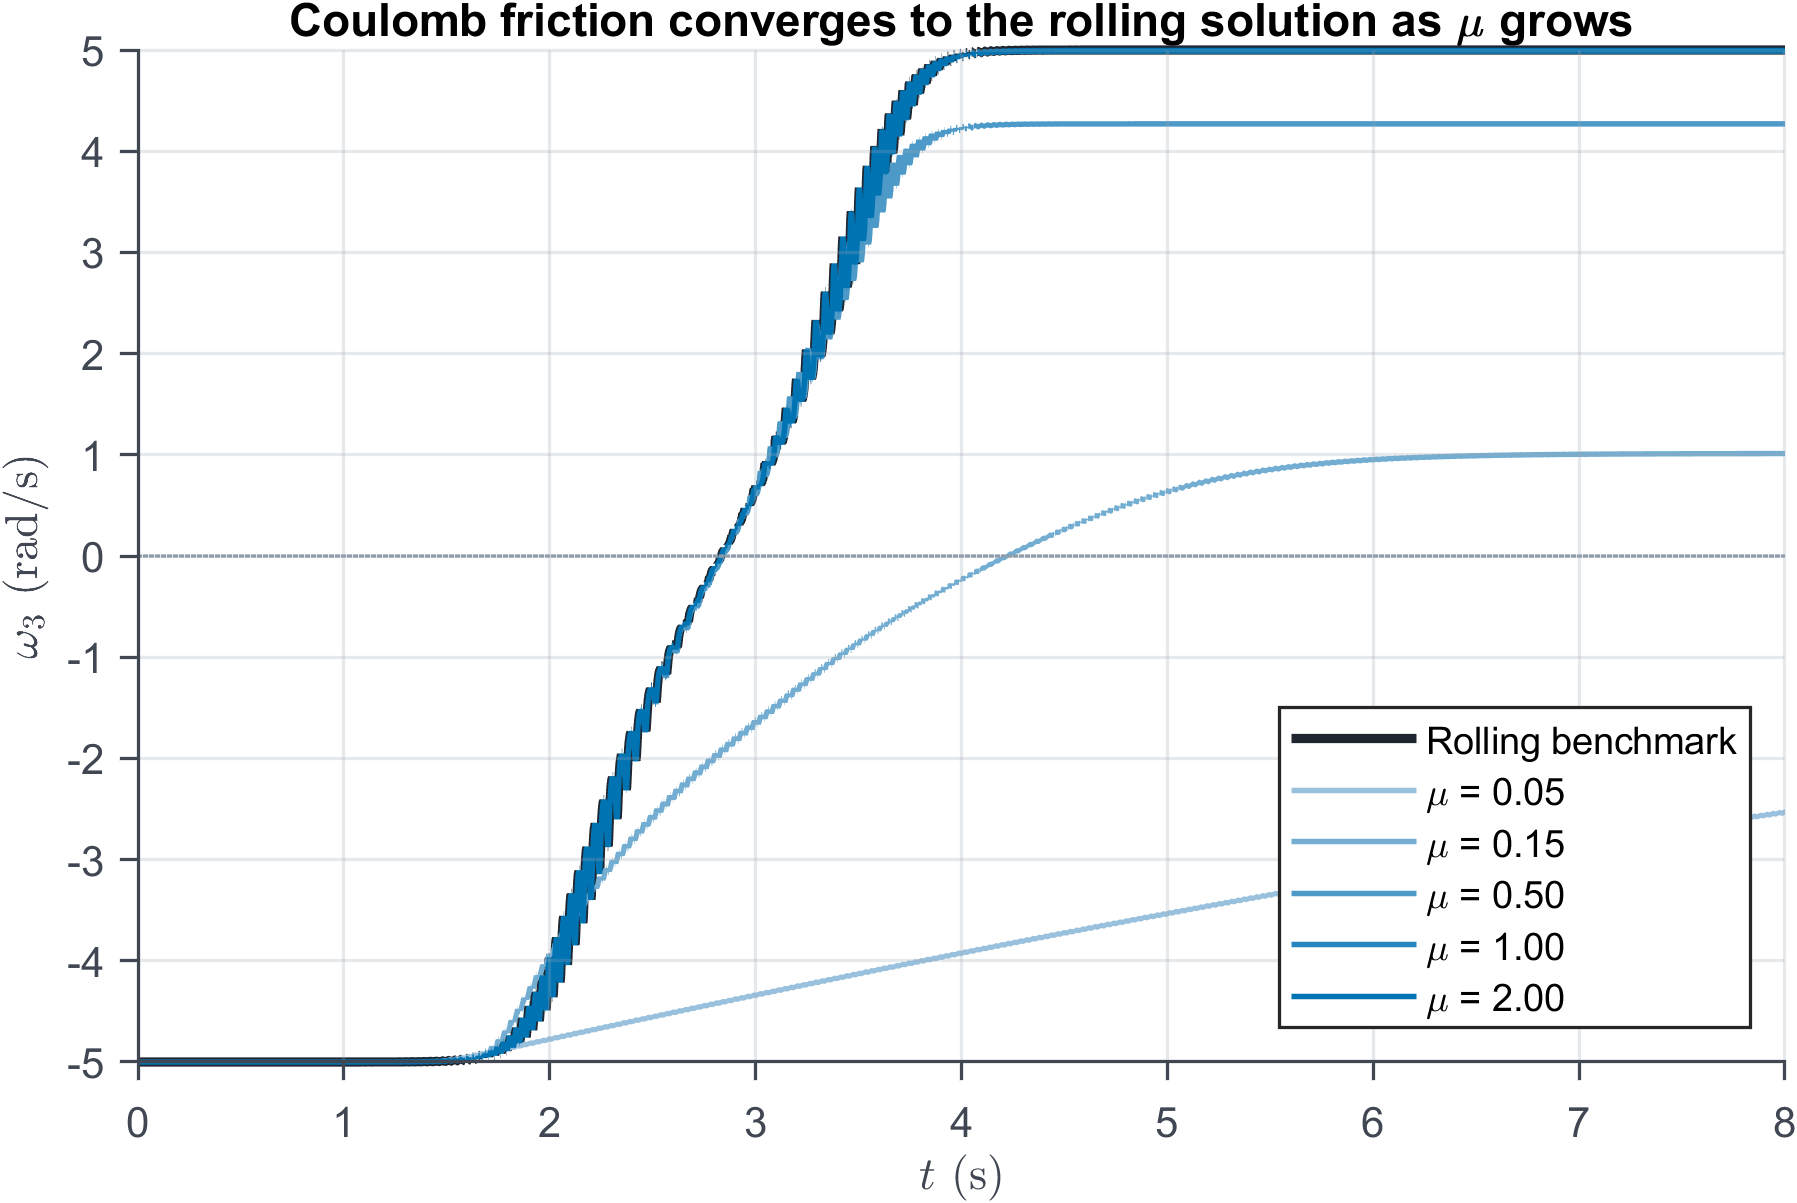
\includegraphics[width=\columnwidth]{figs/sweep_mu.png}
\caption{Spin $\omega_3$ under Coulomb friction for increasing $\mu$, non-preferred
sense, with the rolling solution (thick line).}
\label{fig:mu}
\end{figure}

Figure~\ref{fig:mu} shows the Coulomb solution for increasing friction coefficient.
For $\mu=0.05$ the friction force is too weak to couple the rocking to the spin: the
spin has only fallen to $-2.53$\,rad\,s$^{-1}$ by $t=8$\,s and no reversal occurs. At
$\mu=0.15$ the reversal occurs at $4.22$\,s. For $\mu\ge0.5$ the reversal time is
$2.83$--$2.84$\,s, equal to the rolling value, and the recovered spin approaches the
rolling value of $5$\,rad\,s$^{-1}$, reaching $4.27$\,rad\,s$^{-1}$ at $\mu=0.5$ and
$4.99$\,rad\,s$^{-1}$ at $\mu=1$. The normal reaction approaches the rolling range at the
same time, with a maximum of $4.89\,mg$ at $\mu=0.5$ and $5.76\,mg$ at $\mu=1$, against
$5.86\,mg$ for rolling. Once $\mu$ exceeds the friction demand of about $0.8$ found in
Sec.~\ref{sec:normalresults}, the contact can sustain rolling throughout and the slipping
solution follows the rolling one closely. This convergence is the rolling-limit check of
Sec.~\ref{sec:validation}.

\subsection{Dependence on the initial spin}

\begin{figure}[!tbp]
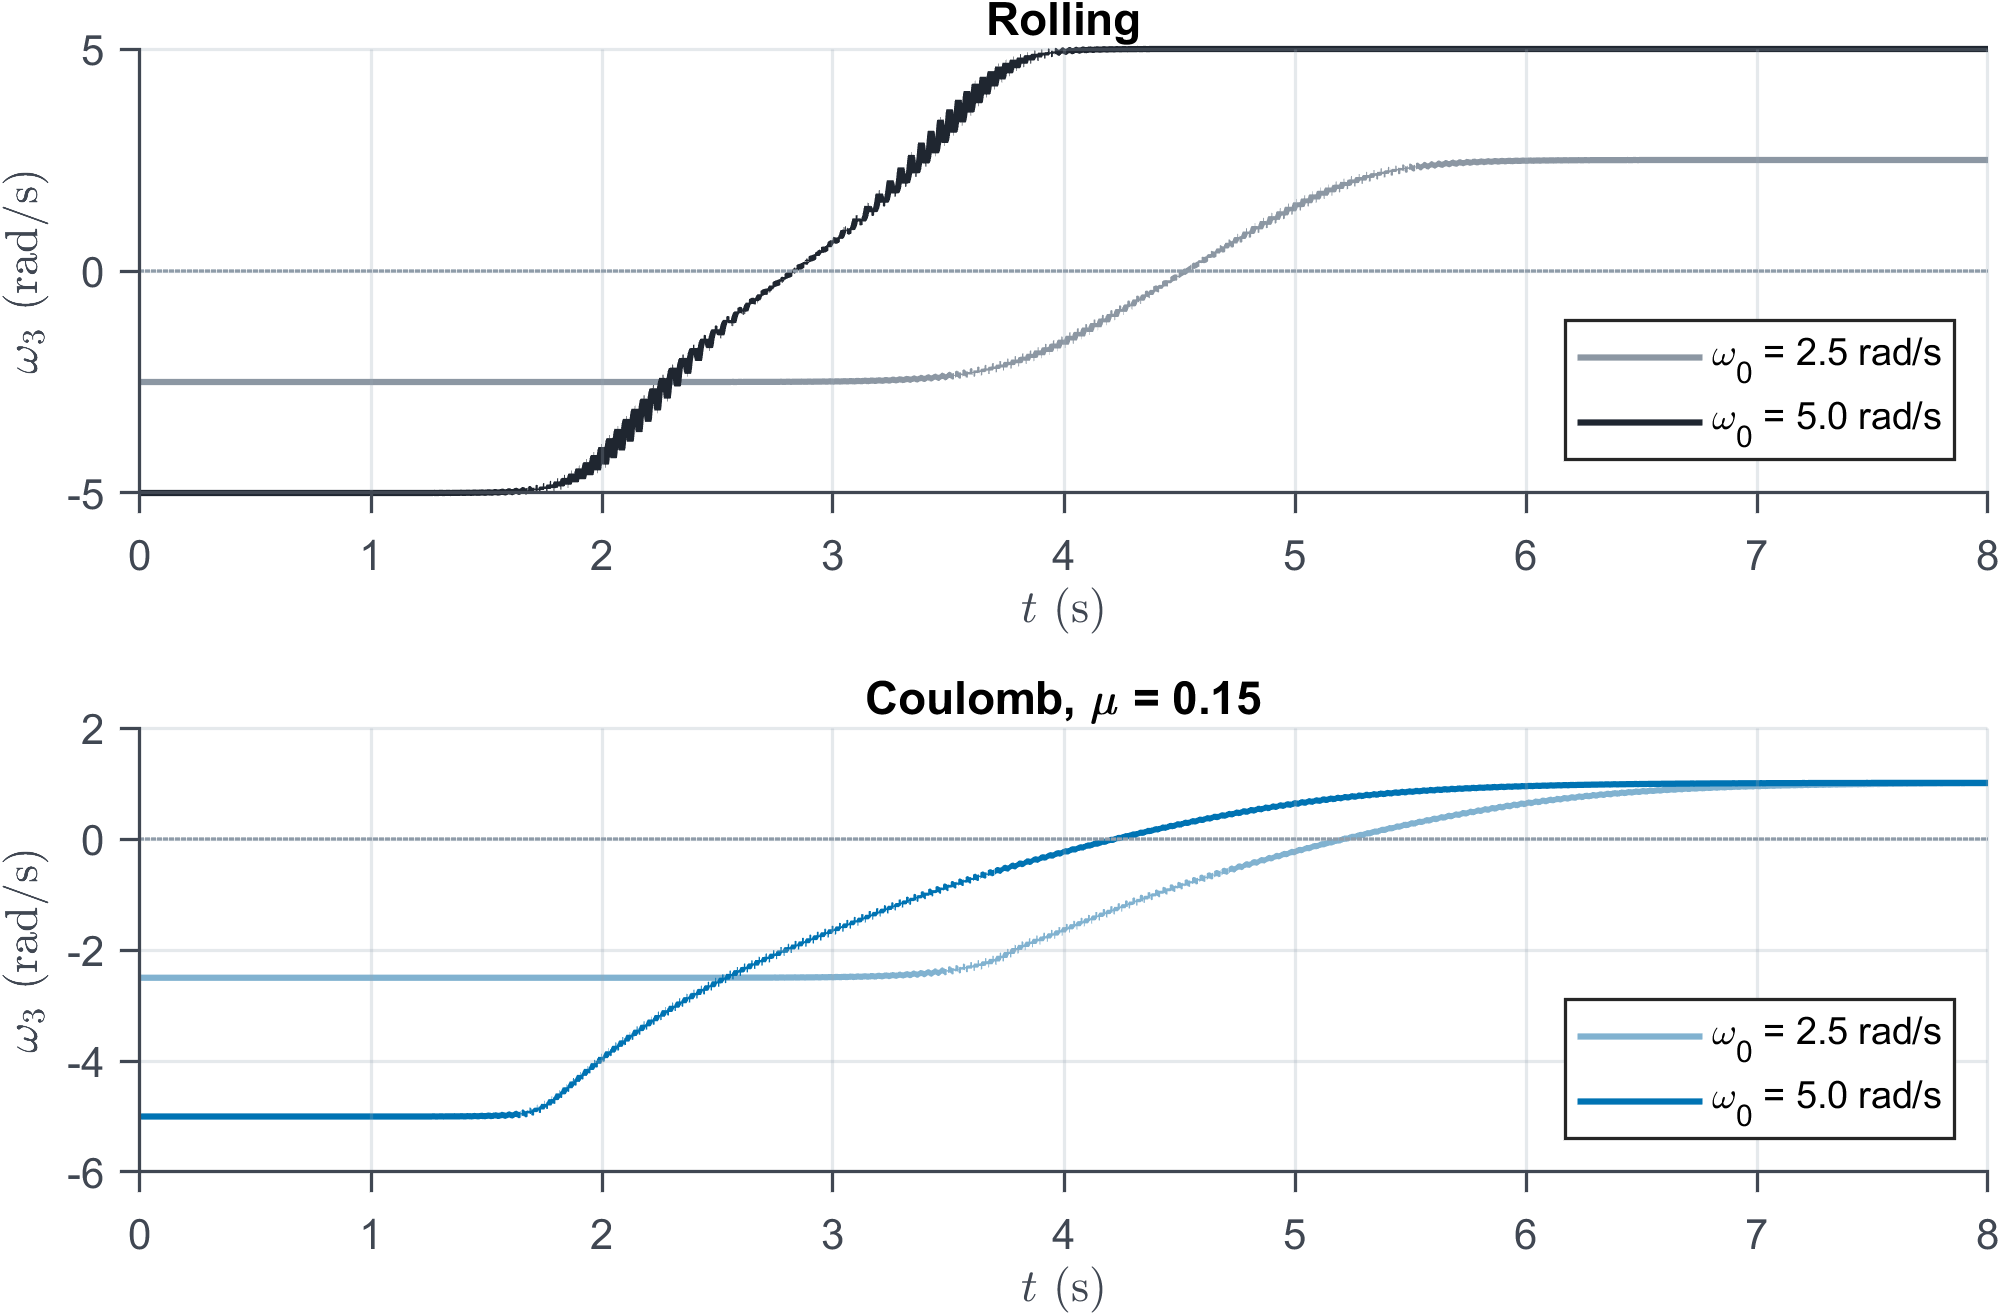
\includegraphics[width=\columnwidth]{figs/compare_initial_spin.png}
\caption{Spin $\omega_3$ for two initial spins in the non-preferred sense. Top: rolling.
Bottom: Coulomb friction, $\mu=0.15$.}
\label{fig:w0}
\end{figure}

Figure~\ref{fig:w0} compares two initial spins in the non-preferred sense. In the
rolling model the smaller spin reverses later, at $4.53$\,s for
$|\omega_0|=2.5$\,rad\,s$^{-1}$ against $2.83$\,s for $5$\,rad\,s$^{-1}$, because the
rocking instability grows more slowly at lower spin. Coulomb friction preserves this
ordering, with reversals at $5.21$ and $4.22$\,s. The final states differ more
strikingly. The conservative rolling model returns the initial magnitude, $2.50$ and
$5.00$\,rad\,s$^{-1}$, whereas under Coulomb friction both cases settle at about
$1.01$\,rad\,s$^{-1}$, almost independently of the initial spin. This suggests that, with
friction, the spin left after reversal is set mainly by the dissipation during the rocking phase rather
than by the initial condition.

\subsection{Comparison of the angular velocities}

\begin{figure*}[!tbp]
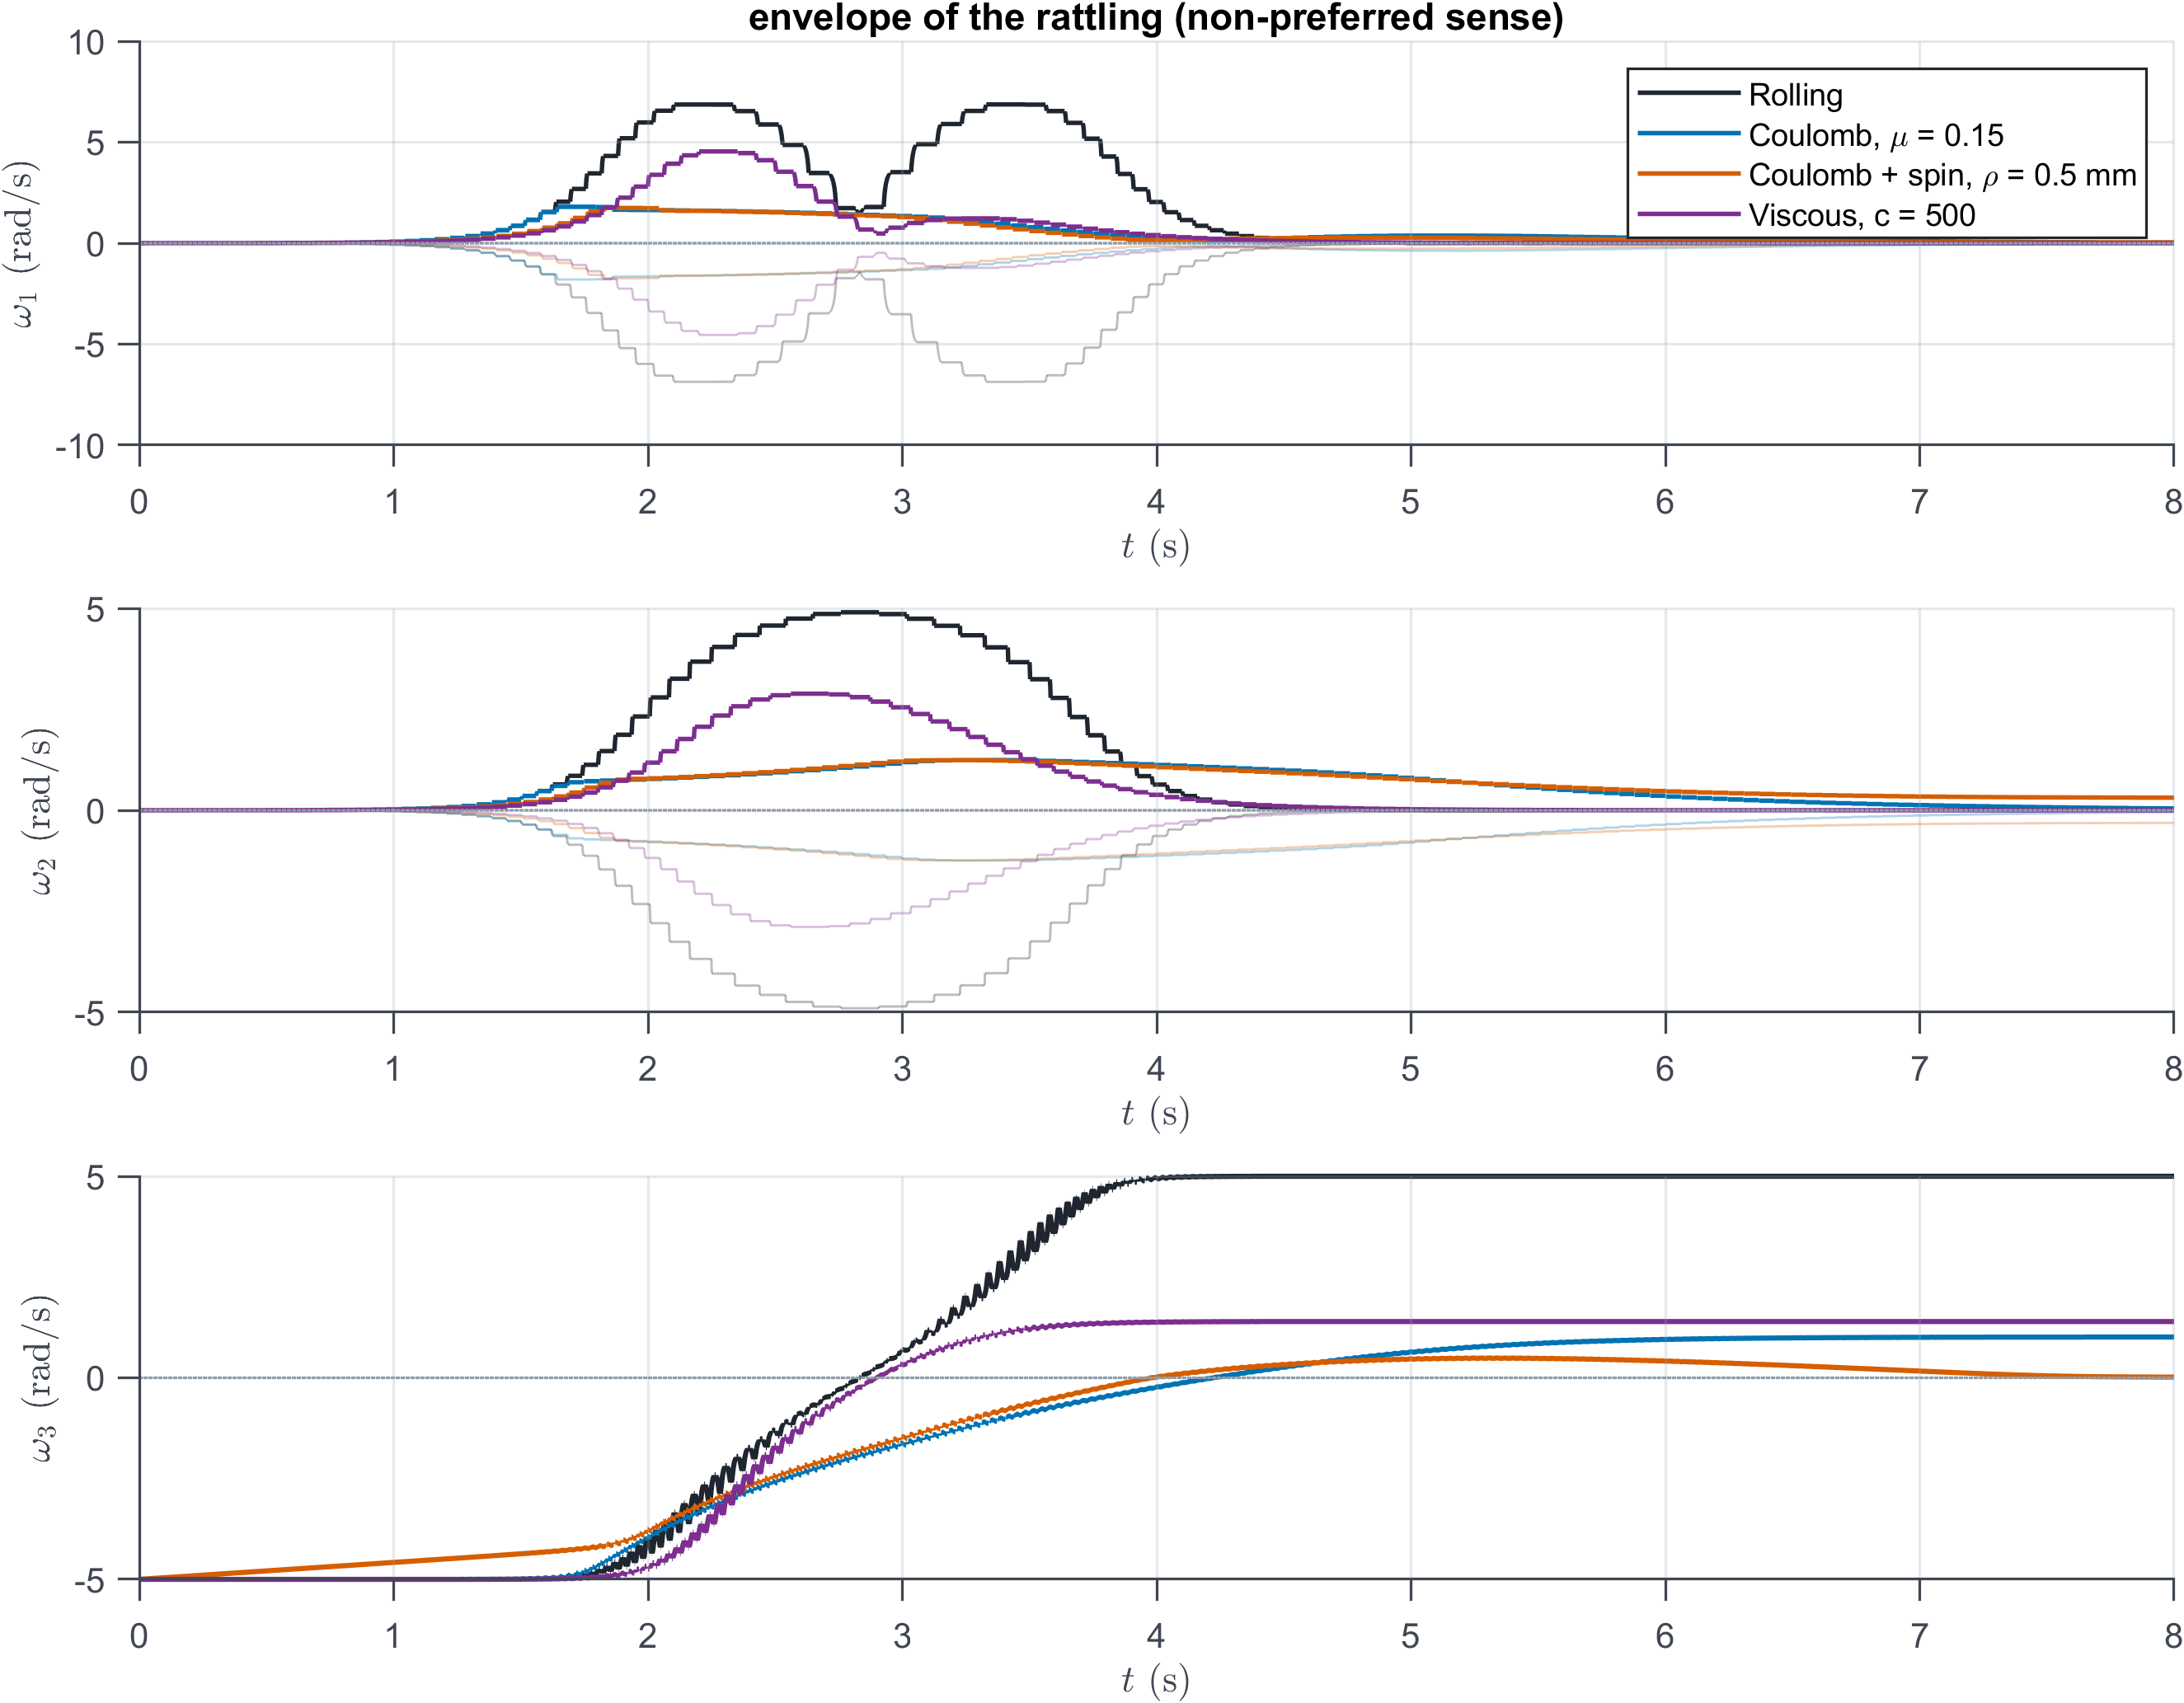
\includegraphics[width=0.92\textwidth]{figs/comparison_omega.png}
\caption{Angular velocity components for the four contact models, non-preferred sense.
For $\omega_1$ and $\omega_2$ the upper envelope of the rocking oscillation is drawn,
with its mirror image faded. The models agree on $\omega_3$ until the instability
develops and then differ in the amplitude and duration of the rocking, which is where
the friction laws remove energy.}
\label{fig:comparisonomega}
\end{figure*}

Figure~\ref{fig:comparisonomega} compares the angular velocities of the four models. The
ordering of the rocking amplitude in $\omega_1$, rolling $>$ viscous $>$ Coulomb
$\approx$ Coulomb with drilling, is the ordering of dissipation at the contact. All four
models share the same underlying instability. They differ in how much of the energy
released into the rocking is returned to the spin and how much is lost.

\subsection{Animations}

\begin{figure}[!tbp]
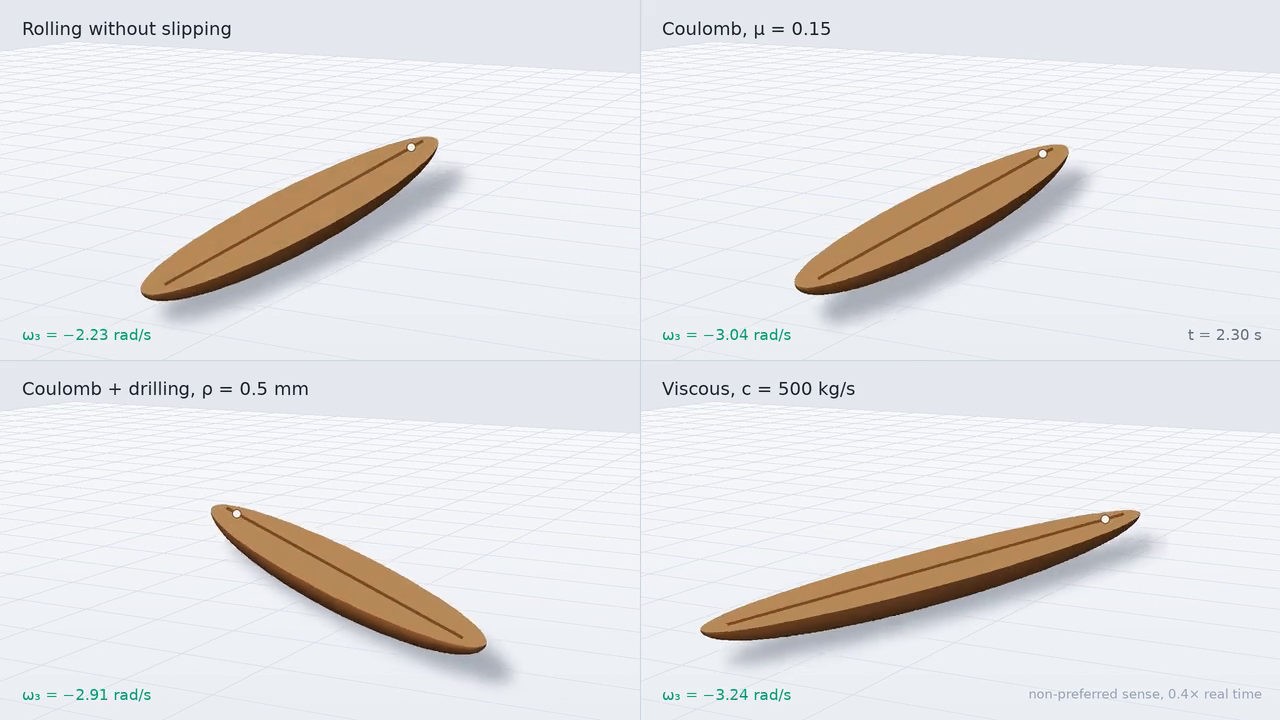
\includegraphics[width=\columnwidth]{figs/anim_grid.png}
\caption{Frame at $t=2.3$\,s from the synchronized animation of the four contact models,
non-preferred sense \cite{SM}. Each body is drawn at its true dimensions and at its
computed height $h(\ve n)$. The tilt is not exaggerated: the rolling body is near its
$6.5^\circ$ peak while the Coulomb body rocks by less than $1^\circ$.}
\label{fig:anim}
\end{figure}

Figure~\ref{fig:anim} shows the four models at the same instant. The full animations
(Appendix~\ref{app:anim}) make two of the results directly visible: the rolling body
rocks strongly and recovers its full spin, whereas the Coulomb body rocks weakly and comes
almost to rest.

%=======================================================================
\section{Limitations}\label{sec:limits}
%=======================================================================

The model assumes a rigid, unilateral point contact that is never lost, with dissipation
only through tangential slip and, optionally, drilling. Several effects are not
included. The drilling torque, Eq.~\eqref{eq:drill}, uses a single effective lever arm
rather than the integral Coulomb--Contensou model or its Pad\'e approximants
\cite{Contensou1963,Zhuravlev1998,Kudra2015}. Rolling resistance, which arises from an
asymmetric pressure distribution over a finite patch and shifts the line of action of the
normal reaction, is neglected, as is contact compliance. If $N$ were to become negative
the body would lose contact and an impact model would be needed; this did not occur in
any run reported here, and the code flags any such violation in its output. The
friction coefficient is constant, and aerodynamic drag, small for dense bodies
\cite{Garcia1988}, is omitted. Finally, the Coulomb results depend on the regularization
velocity unless it is well below the physical slip speeds (Sec.~\ref{sec:eps}). This is
the largest numerical uncertainty, and converged values are quoted throughout.

%=======================================================================
\section{Conclusions}\label{sec:conclusions}
%=======================================================================

We have extended a rolling description of the rattleback to a contact that can slip and
compared three tangential contact laws. The main findings are as follows.

(1) Friction cannot be added to a rolling model of the rattleback, because the slip
velocity vanishes identically under rolling. The constraint has to be released, which
raises the system from six to nine states and requires the contact force to be computed
explicitly.

(2) The normal reaction must be solved from the contact condition rather than set equal
to $mg$. Equation~\eqref{eq:N} gives it in closed form at the cost of one scalar
division. In the rolling solution it varies between $0.20\,mg$ and $5.86\,mg$, and the
approximation $N=mg$ produces a $14\%$ error in the reversal time near the rolling limit
while preventing convergence to that limit.

(3) The slipping formulation reproduces the rolling solution to three significant
figures as $\mu$ grows, satisfies the contact condition to solver tolerance, and
dissipates energy monotonically for every friction law tested.

(4) Coulomb friction at $\mu=0.15$ delays the reversal from $2.83$ to $4.22$\,s, limits
the rocking to $0.84^\circ$, and dissipates $12\%$ of the initial energy, producing a
single reversal to a reduced spin instead of the conservative behavior of the rolling
model.

(5) The Coulomb and viscous laws differ structurally, not only quantitatively. Because the
viscous force vanishes with the slip, a viscous coefficient of comparable nominal size
produces no reversal at all, and the rolling behavior is recovered only as
$c_v\to\infty$. This is the counterpart, for the rattleback, of the finite-time and
asymptotic transitions obtained by Moffatt and Shimomura.

(6) Drilling friction is strongly sensitive to the contact patch. With a Hertzian lever
arm, $\rho\approx0.5$\,mm, the reversal survives and the body then spins down, in both
senses, as a real celt does. At $\rho=2$\,mm the drilling torque stops the body before
the instability can develop, and the rattleback effect is suppressed.

\section*{Data availability}

The MATLAB source code that produced the figures, the Python implementation used for the
cross-check and the animations, and six animations are openly available as Supplemental
Material \cite{SM}.

\appendix

\section{Animations and code}\label{app:anim}

The Supplemental Material \cite{SM} contains six animations, each for
$|\omega_0|=5$\,rad\,s$^{-1}$ over the first $6$\,s of motion: rolling without slipping
in the non-preferred sense; rolling in the preferred and non-preferred senses side by
side; Coulomb friction with $\mu=0.15$; Coulomb friction with drilling torque,
$\rho=0.5$\,mm; viscous friction with $c_v=500$\,kg\,s$^{-1}$; and all four contact
models synchronized in a $2\times2$ grid. Playback is at $0.4$ times real time so that the
$11$\,Hz rocking is resolved at $40$ frames per second. Each single-model animation shows
the body together with $\omega_i(t)$ and $\theta(t)$ traced as time advances, and no
deflection is exaggerated.

The MATLAB program \texttt{rattleback\_simulator\_123H.m} integrates all four contact
models for both senses of the initial spin, performs the sweeps in $\varepsilon$, $\rho$,
$\mu$, and $\omega_0$ and the comparison with $N\equiv mg$, prints the verification
checks, and exports every figure in this paper except Figs.~\ref{fig:schematic} and
\ref{fig:anim}.

\begin{thebibliography}{99}

\bibitem{Walker1896} G.~T. Walker, Q. J. Pure Appl. Math. \textbf{28}, 175 (1896).

\bibitem{Bondi1986} H. Bondi, Proc. R. Soc. Lond. A \textbf{405}, 265 (1986).

\bibitem{Markeev1983} A.~P. Markeev, Prikl. Mat. Mekh. \textbf{47}, 575 (1983).

\bibitem{Pascal1983} M. Pascal, Prikl. Mat. Mekh. \textbf{47}, 321 (1983).

\bibitem{Moffatt2008} H.~K. Moffatt and T. Tokieda, Proc. R. Soc. Edinb. A \textbf{138}, 361 (2008).

\bibitem{Kane1982} T.~R. Kane and D.~A. Levinson, Int. J. Non-Linear Mech. \textbf{17}, 175 (1982).

\bibitem{Lindberg1983} R.~E. Lindberg, Jr. and R.~W. Longman, Acta Mech. \textbf{49}, 81 (1983).

\bibitem{Garcia1988} A. Garcia and M. Hubbard, Proc. R. Soc. Lond. A \textbf{418}, 165 (1988).

\bibitem{Borisov2003} A.~V. Borisov and I.~S. Mamaev, Phys. Usp. \textbf{46}, 393 (2003).

\bibitem{Kondo2017} Y. Kondo and H. Nakanishi, Phys. Rev. E \textbf{95}, 062207 (2017).

\bibitem{Mukherjee} D. Mukherjee, \textit{On Preferential Rotation of the Rattleback},
lecture notes, Department of Mechanical Engineering, Indian Institute of Technology Kanpur
(unpublished).

\bibitem{Takano2014} H. Takano, Regul. Chaotic Dyn. \textbf{19}, 81 (2014).

\bibitem{Kudra2015} G. Kudra and J. Awrejcewicz, Acta Mech. \textbf{226}, 2831 (2015).

\bibitem{Moffatt2002} H.~K. Moffatt and Y. Shimomura, Nature (London) \textbf{416}, 385 (2002).

\bibitem{Stewart2000} D.~E. Stewart, SIAM Rev. \textbf{42}, 3 (2000).

\bibitem{Contensou1963} P. Contensou, in \textit{Kreiselprobleme/Gyrodynamics, IUTAM
Symposium, Celerina, 1962}, edited by H. Ziegler (Springer, Berlin, 1963), pp.~201--216.

\bibitem{Zhuravlev1998} V.~F. Zhuravlev, J. Appl. Math. Mech. \textbf{62}, 705 (1998).

\bibitem{Johnson1985} K.~L. Johnson, \textit{Contact Mechanics} (Cambridge University
Press, Cambridge, England, 1985).

\bibitem{Shampine1997} L.~F. Shampine and M.~W. Reichelt, SIAM J. Sci. Comput.
\textbf{18}, 1 (1997).

\bibitem{Eaton2023} J.~W. Eaton, D. Bateman, S. Hauberg, and R. Wehbring,
\textit{GNU Octave Version 8.4.0 Manual: A High-Level Interactive Language for Numerical
Computations} (2023).

\bibitem{Petzold1983} L. Petzold, SIAM J. Sci. Stat. Comput. \textbf{4}, 136 (1983).

\bibitem{Virtanen2020} P. Virtanen \textit{et al.}, Nat. Methods \textbf{17}, 261 (2020).

\bibitem{SM} See Supplemental Material at \url{\supp} for six animations and the source
code (MATLAB and Python).

\end{thebibliography}

\end{document}
